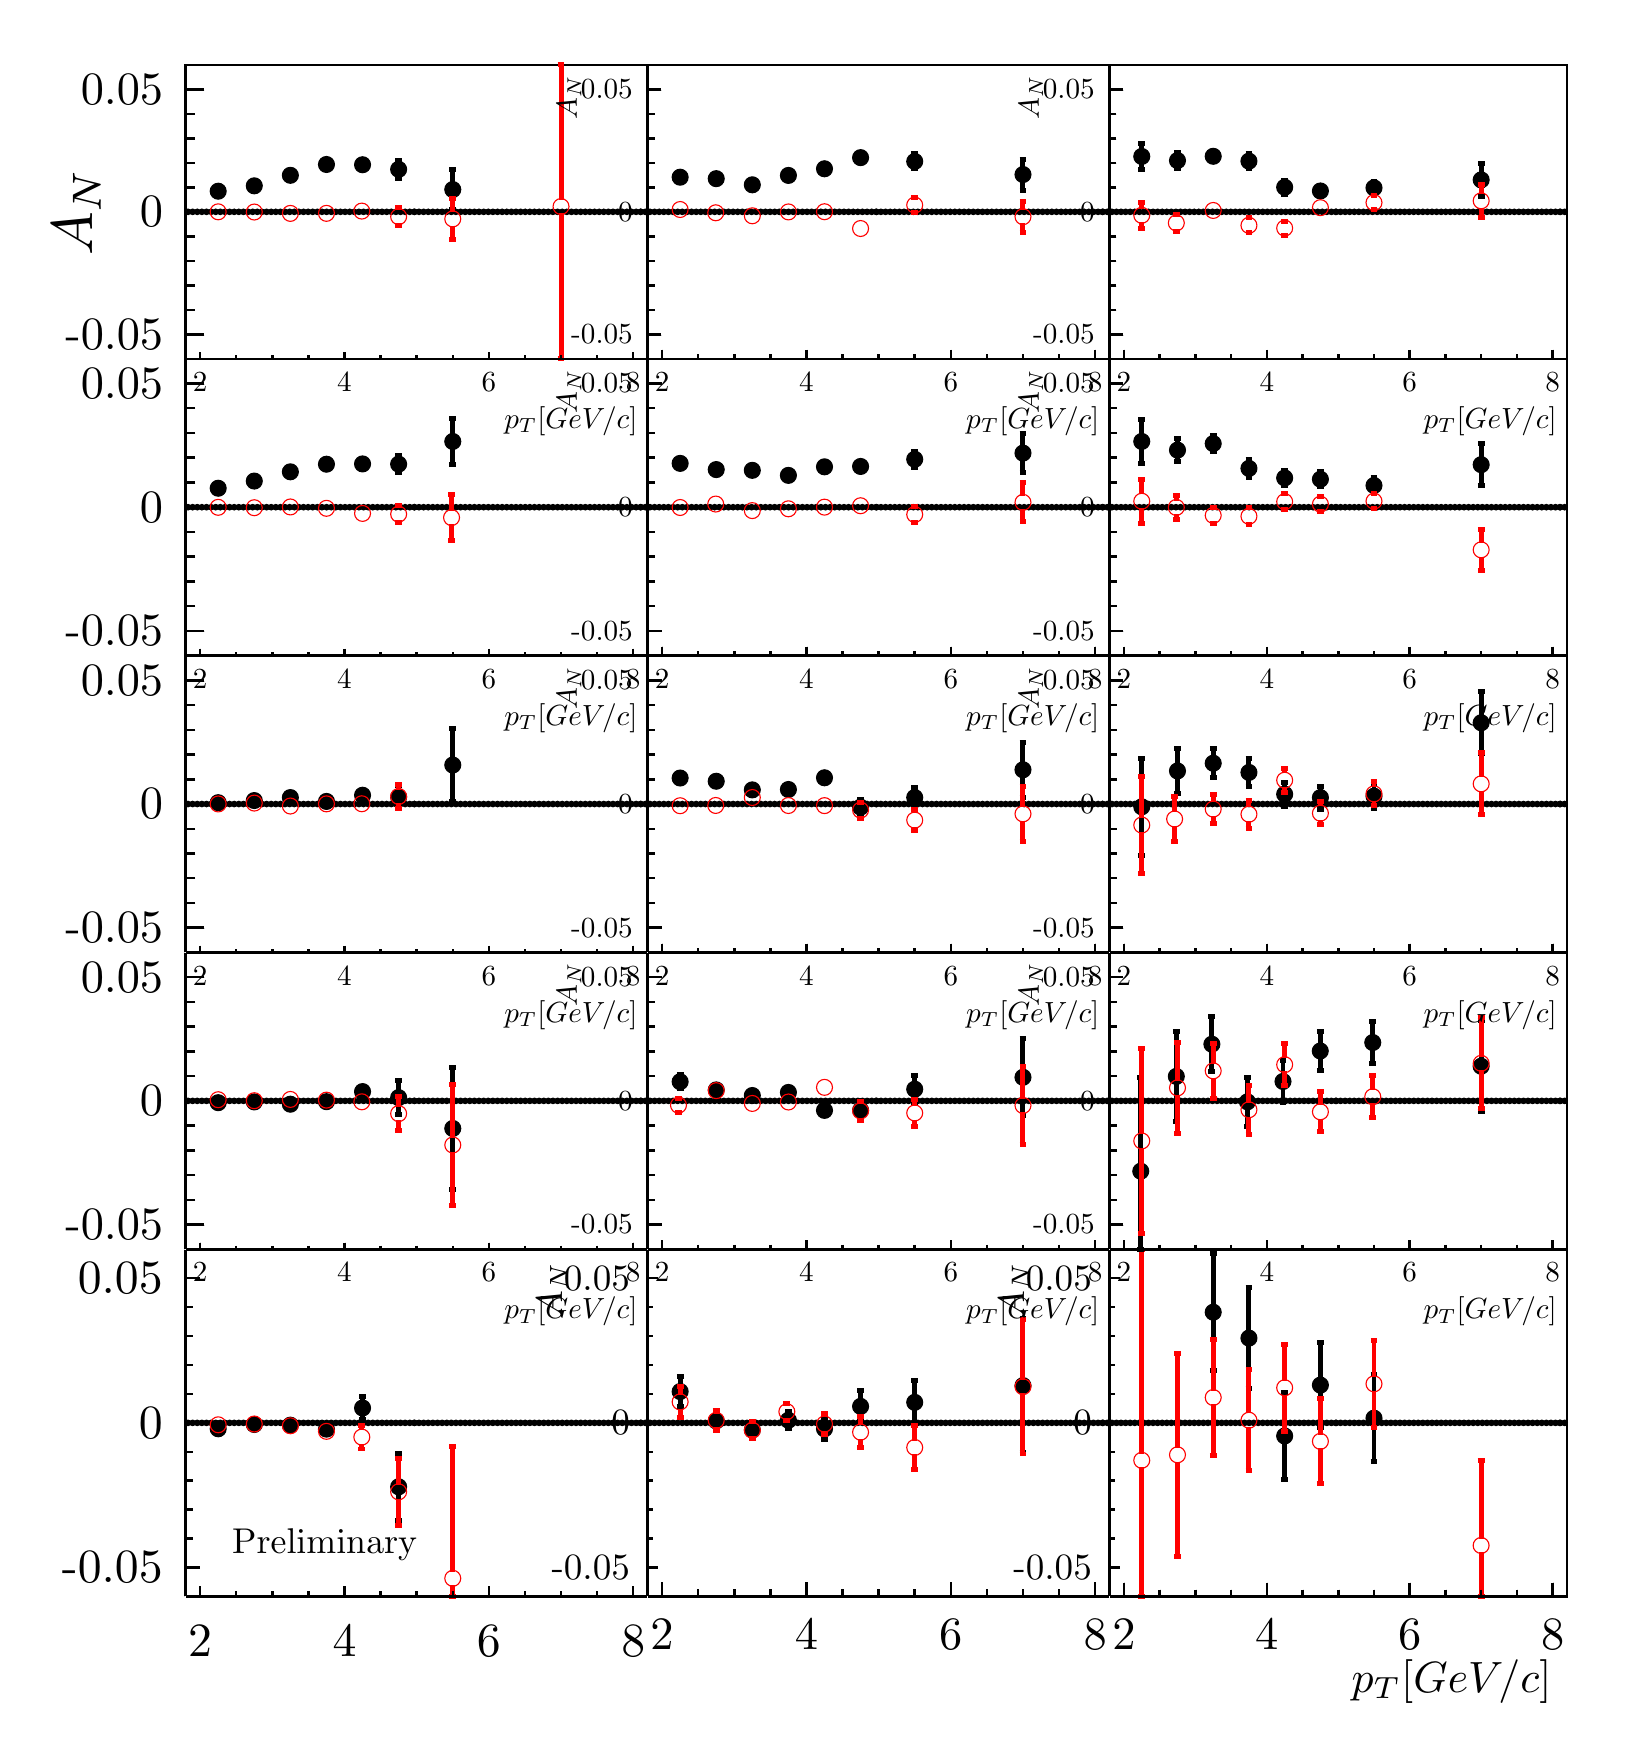
\begin{tikzpicture}
\pgfdeclareplotmark{cross} {
\pgfpathmoveto{\pgfpoint{-0.3\pgfplotmarksize}{\pgfplotmarksize}}
\pgfpathlineto{\pgfpoint{+0.3\pgfplotmarksize}{\pgfplotmarksize}}
\pgfpathlineto{\pgfpoint{+0.3\pgfplotmarksize}{0.3\pgfplotmarksize}}
\pgfpathlineto{\pgfpoint{+1\pgfplotmarksize}{0.3\pgfplotmarksize}}
\pgfpathlineto{\pgfpoint{+1\pgfplotmarksize}{-0.3\pgfplotmarksize}}
\pgfpathlineto{\pgfpoint{+0.3\pgfplotmarksize}{-0.3\pgfplotmarksize}}
\pgfpathlineto{\pgfpoint{+0.3\pgfplotmarksize}{-1.\pgfplotmarksize}}
\pgfpathlineto{\pgfpoint{-0.3\pgfplotmarksize}{-1.\pgfplotmarksize}}
\pgfpathlineto{\pgfpoint{-0.3\pgfplotmarksize}{-0.3\pgfplotmarksize}}
\pgfpathlineto{\pgfpoint{-1.\pgfplotmarksize}{-0.3\pgfplotmarksize}}
\pgfpathlineto{\pgfpoint{-1.\pgfplotmarksize}{0.3\pgfplotmarksize}}
\pgfpathlineto{\pgfpoint{-0.3\pgfplotmarksize}{0.3\pgfplotmarksize}}
\pgfpathclose
\pgfusepathqstroke
}
\pgfdeclareplotmark{cross*} {
\pgfpathmoveto{\pgfpoint{-0.3\pgfplotmarksize}{\pgfplotmarksize}}
\pgfpathlineto{\pgfpoint{+0.3\pgfplotmarksize}{\pgfplotmarksize}}
\pgfpathlineto{\pgfpoint{+0.3\pgfplotmarksize}{0.3\pgfplotmarksize}}
\pgfpathlineto{\pgfpoint{+1\pgfplotmarksize}{0.3\pgfplotmarksize}}
\pgfpathlineto{\pgfpoint{+1\pgfplotmarksize}{-0.3\pgfplotmarksize}}
\pgfpathlineto{\pgfpoint{+0.3\pgfplotmarksize}{-0.3\pgfplotmarksize}}
\pgfpathlineto{\pgfpoint{+0.3\pgfplotmarksize}{-1.\pgfplotmarksize}}
\pgfpathlineto{\pgfpoint{-0.3\pgfplotmarksize}{-1.\pgfplotmarksize}}
\pgfpathlineto{\pgfpoint{-0.3\pgfplotmarksize}{-0.3\pgfplotmarksize}}
\pgfpathlineto{\pgfpoint{-1.\pgfplotmarksize}{-0.3\pgfplotmarksize}}
\pgfpathlineto{\pgfpoint{-1.\pgfplotmarksize}{0.3\pgfplotmarksize}}
\pgfpathlineto{\pgfpoint{-0.3\pgfplotmarksize}{0.3\pgfplotmarksize}}
\pgfpathclose
\pgfusepathqfillstroke
}
\pgfdeclareplotmark{newstar} {
\pgfpathmoveto{\pgfqpoint{0pt}{\pgfplotmarksize}}
\pgfpathlineto{\pgfqpointpolar{44}{0.5\pgfplotmarksize}}
\pgfpathlineto{\pgfqpointpolar{18}{\pgfplotmarksize}}
\pgfpathlineto{\pgfqpointpolar{-20}{0.5\pgfplotmarksize}}
\pgfpathlineto{\pgfqpointpolar{-54}{\pgfplotmarksize}}
\pgfpathlineto{\pgfqpointpolar{-90}{0.5\pgfplotmarksize}}
\pgfpathlineto{\pgfqpointpolar{234}{\pgfplotmarksize}}
\pgfpathlineto{\pgfqpointpolar{198}{0.5\pgfplotmarksize}}
\pgfpathlineto{\pgfqpointpolar{162}{\pgfplotmarksize}}
\pgfpathlineto{\pgfqpointpolar{134}{0.5\pgfplotmarksize}}
\pgfpathclose
\pgfusepathqstroke
}
\pgfdeclareplotmark{newstar*} {
\pgfpathmoveto{\pgfqpoint{0pt}{\pgfplotmarksize}}
\pgfpathlineto{\pgfqpointpolar{44}{0.5\pgfplotmarksize}}
\pgfpathlineto{\pgfqpointpolar{18}{\pgfplotmarksize}}
\pgfpathlineto{\pgfqpointpolar{-20}{0.5\pgfplotmarksize}}
\pgfpathlineto{\pgfqpointpolar{-54}{\pgfplotmarksize}}
\pgfpathlineto{\pgfqpointpolar{-90}{0.5\pgfplotmarksize}}
\pgfpathlineto{\pgfqpointpolar{234}{\pgfplotmarksize}}
\pgfpathlineto{\pgfqpointpolar{198}{0.5\pgfplotmarksize}}
\pgfpathlineto{\pgfqpointpolar{162}{\pgfplotmarksize}}
\pgfpathlineto{\pgfqpointpolar{134}{0.5\pgfplotmarksize}}
\pgfpathclose
\pgfusepathqfillstroke
}
\definecolor{c}{rgb}{0.999,0.999,0.999};
\draw [color=c, fill=c] (0,0) rectangle (20,21.4194);
\definecolor{c}{rgb}{0,0,0};
\draw [anchor=base west] (0.2,0.214194) node[scale=1.09854, color=c, rotate=0]{Tue Oct  6 22:13:36 2020};
\definecolor{c}{rgb}{1,1,1};
\draw [color=c, fill=c] (0,0) rectangle (7.86667,5.91174);
\draw [color=c, fill=c] (2,1.50299) rectangle (7.86667,5.91174);
\definecolor{c}{rgb}{0,0,0};
\draw [c,line width=0.9] (2,1.50299) -- (2,5.91174) -- (7.86667,5.91174) -- (7.86667,1.50299) -- (2,1.50299);
\definecolor{c}{rgb}{1,1,1};
\draw [color=c, fill=c] (2,1.50299) rectangle (7.86667,5.91174);
\definecolor{c}{rgb}{0,0,0};
\draw [c,line width=0.9] (2,1.50299) -- (2,5.91174) -- (7.86667,5.91174) -- (7.86667,1.50299) -- (2,1.50299);
\foreach \P in
 {(2.02933,3.70736),(2.088,3.70736),(2.14667,3.70736),(2.20533,3.70736),(2.264,3.70736),(2.32267,3.70736),(2.38133,3.70736),(2.44,3.70736),(2.49867,3.70736),(2.55733,3.70736),(2.616,3.70736),(2.67467,3.70736),(2.73333,3.70736),(2.792,3.70736),(2.8506
7,3.70736),(2.90933,3.70736),(2.968,3.70736),(3.02667,3.70736),(3.08533,3.70736),(3.144,3.70736),(3.20267,3.70736),(3.26133,3.70736),(3.32,3.70736),(3.37867,3.70736),(3.43733,3.70736),(3.496,3.70736),(3.55467,3.70736),(3.61333,3.70736),(3.672,3.70736
),(3.73067,3.70736),(3.78933,3.70736),(3.848,3.70736),(3.90667,3.70736),(3.96533,3.70736),(4.024,3.70736),(4.08267,3.70736),(4.14133,3.70736),(4.2,3.70736),(4.25867,3.70736),(4.31733,3.70736),(4.376,3.70736),(4.43467,3.70736),(4.49333,3.70736),(4.552
,3.70736),(4.61067,3.70736),(4.66933,3.70736),(4.728,3.70736),(4.78667,3.70736),(4.84533,3.70736),(4.904,3.70736)}{\draw[mark options={color=c,fill=c},mark size=2.402402pt,mark=*,mark size=1pt] plot coordinates {\P};}
\foreach \P in
 {(4.904,3.70736),(4.96267,3.70736),(5.02133,3.70736),(5.08,3.70736),(5.13867,3.70736),(5.19733,3.70736),(5.256,3.70736),(5.31467,3.70736),(5.37333,3.70736),(5.432,3.70736),(5.49067,3.70736),(5.54933,3.70736),(5.608,3.70736),(5.66667,3.70736),(5.7253
3,3.70736),(5.784,3.70736),(5.84267,3.70736),(5.90133,3.70736),(5.96,3.70736),(6.01867,3.70736),(6.07733,3.70736),(6.136,3.70736),(6.19467,3.70736),(6.25333,3.70736),(6.312,3.70736),(6.37067,3.70736),(6.42933,3.70736),(6.488,3.70736),(6.54667,3.70736
),(6.60533,3.70736),(6.664,3.70736),(6.72267,3.70736),(6.78133,3.70736),(6.84,3.70736),(6.89867,3.70736),(6.95733,3.70736),(7.016,3.70736),(7.07467,3.70736),(7.13333,3.70736),(7.192,3.70736),(7.25067,3.70736),(7.30933,3.70736),(7.368,3.70736),(7.4266
7,3.70736),(7.48533,3.70736),(7.544,3.70736),(7.60267,3.70736),(7.66133,3.70736),(7.72,3.70736),(7.77867,3.70736)}{\draw[mark options={color=c,fill=c},mark size=2.402402pt,mark=*,mark size=1pt] plot coordinates {\P};}
\foreach \P in {(7.77867,3.70736),(7.83733,3.70736)}{\draw[mark options={color=c,fill=c},mark size=2.402402pt,mark=*,mark size=1pt] plot coordinates {\P};}
\draw [c,line width=0.9] (2,1.50299) -- (7.86667,1.50299);
\draw [c,line width=0.9] (2.18333,1.63525) -- (2.18333,1.50299);
\draw [c,line width=0.9] (2.64167,1.56912) -- (2.64167,1.50299);
\draw [c,line width=0.9] (3.1,1.56912) -- (3.1,1.50299);
\draw [c,line width=0.9] (3.55833,1.56912) -- (3.55833,1.50299);
\draw [c,line width=0.9] (4.01667,1.63525) -- (4.01667,1.50299);
\draw [c,line width=0.9] (4.475,1.56912) -- (4.475,1.50299);
\draw [c,line width=0.9] (4.93333,1.56912) -- (4.93333,1.50299);
\draw [c,line width=0.9] (5.39167,1.56912) -- (5.39167,1.50299);
\draw [c,line width=0.9] (5.85,1.63525) -- (5.85,1.50299);
\draw [c,line width=0.9] (6.30833,1.56912) -- (6.30833,1.50299);
\draw [c,line width=0.9] (6.76667,1.56912) -- (6.76667,1.50299);
\draw [c,line width=0.9] (7.225,1.56912) -- (7.225,1.50299);
\draw [c,line width=0.9] (7.68333,1.63525) -- (7.68333,1.50299);
\draw [c,line width=0.9] (2.18333,1.63525) -- (2.18333,1.50299);
\draw [c,line width=0.9] (7.68333,1.63525) -- (7.68333,1.50299);
\draw [anchor=base] (2.18333,0.740371) node[scale=1.72508, color=c, rotate=0]{2};
\draw [anchor=base] (4.01667,0.740371) node[scale=1.72508, color=c, rotate=0]{4};
\draw [anchor=base] (5.85,0.740371) node[scale=1.72508, color=c, rotate=0]{6};
\draw [anchor=base] (7.68333,0.740371) node[scale=1.72508, color=c, rotate=0]{8};
\draw [c,line width=0.9] (2,1.50299) -- (2,5.91174);
\draw [c,line width=0.9] (2.176,1.87038) -- (2,1.87038);
\draw [c,line width=0.9] (2.088,2.23778) -- (2,2.23778);
\draw [c,line width=0.9] (2.088,2.60517) -- (2,2.60517);
\draw [c,line width=0.9] (2.088,2.97257) -- (2,2.97257);
\draw [c,line width=0.9] (2.088,3.33997) -- (2,3.33997);
\draw [c,line width=0.9] (2.176,3.70736) -- (2,3.70736);
\draw [c,line width=0.9] (2.088,4.07476) -- (2,4.07476);
\draw [c,line width=0.9] (2.088,4.44216) -- (2,4.44216);
\draw [c,line width=0.9] (2.088,4.80955) -- (2,4.80955);
\draw [c,line width=0.9] (2.088,5.17695) -- (2,5.17695);
\draw [c,line width=0.9] (2.176,5.54435) -- (2,5.54435);
\draw [c,line width=0.9] (2.176,1.87038) -- (2,1.87038);
\draw [c,line width=0.9] (2.088,1.50299) -- (2,1.50299);
\draw [c,line width=0.9] (2.176,5.54435) -- (2,5.54435);
\draw [c,line width=0.9] (2.088,5.91174) -- (2,5.91174);
\draw [anchor= east] (1.92133,1.87038) node[scale=1.72508, color=c, rotate=0]{-0.05};
\draw [anchor= east] (1.92133,3.70736) node[scale=1.72508, color=c, rotate=0]{0};
\draw [anchor= east] (1.92133,5.54435) node[scale=1.72508, color=c, rotate=0]{0.05};
\draw [c,line width=1.8] (4.24583,3.98241) -- (4.24583,4.04772);
\draw [c,line width=1.8] (4.20282,4.04772) -- (4.28884,4.04772);
\draw [c,line width=1.8] (4.24583,3.81037) -- (4.24583,3.74505);
\draw [c,line width=1.8] (4.20282,3.74505) -- (4.28884,3.74505);
\draw [c,line width=1.8] (4.70417,2.98135) -- (4.70417,3.31878);
\draw [c,line width=1.8] (4.66116,3.31878) -- (4.74718,3.31878);
\draw [c,line width=1.8] (4.70417,2.8093) -- (4.70417,2.47187);
\draw [c,line width=1.8] (4.66116,2.47187) -- (4.74718,2.47187);
\foreach \P in {(2.4125,3.63218),(2.87083,3.68695),(3.32917,3.67827),(3.7875,3.62764),(4.24583,3.89639),(4.70417,2.89532)}{\draw[mark options={color=c,fill=c},mark size=2.882883pt,mark=*] plot coordinates {\P};}
\definecolor{c}{rgb}{1,0,0};
\draw [c,line width=1.8] (4.23656,3.6129) -- (4.23656,3.67822);
\draw [c,line width=1.8] (4.19355,3.67822) -- (4.27957,3.67822);
\draw [c,line width=1.8] (4.23656,3.44086) -- (4.23656,3.37554);
\draw [c,line width=1.8] (4.19355,3.37554) -- (4.27957,3.37554);
\draw [c,line width=1.8] (4.70417,2.91807) -- (4.70417,3.25555);
\draw [c,line width=1.8] (4.66116,3.25555) -- (4.74718,3.25555);
\draw [c,line width=1.8] (4.70417,2.74602) -- (4.70417,2.40854);
\draw [c,line width=1.8] (4.66116,2.40854) -- (4.74718,2.40854);
\draw [c,line width=1.8] (5.39167,1.81917) -- (5.39167,3.41259);
\draw [c,line width=1.8] (5.34866,3.41259) -- (5.43468,3.41259);
\draw [c,line width=1.8] (5.39167,1.64713) -- (5.39167,1.50299);
\draw [c,line width=1.8] (5.34866,1.50299) -- (5.43468,1.50299);
\foreach \P in {(2.4125,3.68297),(2.87083,3.69276),(3.32917,3.67056),(3.7875,3.59973),(4.23656,3.52688),(4.70417,2.83205),(5.39167,1.73315)}{\draw[mark options={color=c,fill=c},mark size=2.882883pt,mark=o] plot coordinates {\P};}
\definecolor{c}{rgb}{0,0,0};
\draw [anchor=base west] (2.43011,2.04301) node[scale=1.29381, color=c, rotate=0]{Preliminary};
\draw [c,line width=0.9] (2,1.50299) -- (7.86667,1.50299);
\draw [c,line width=0.9] (2.18333,1.63525) -- (2.18333,1.50299);
\draw [c,line width=0.9] (2.64167,1.56912) -- (2.64167,1.50299);
\draw [c,line width=0.9] (3.1,1.56912) -- (3.1,1.50299);
\draw [c,line width=0.9] (3.55833,1.56912) -- (3.55833,1.50299);
\draw [c,line width=0.9] (4.01667,1.63525) -- (4.01667,1.50299);
\draw [c,line width=0.9] (4.475,1.56912) -- (4.475,1.50299);
\draw [c,line width=0.9] (4.93333,1.56912) -- (4.93333,1.50299);
\draw [c,line width=0.9] (5.39167,1.56912) -- (5.39167,1.50299);
\draw [c,line width=0.9] (5.85,1.63525) -- (5.85,1.50299);
\draw [c,line width=0.9] (6.30833,1.56912) -- (6.30833,1.50299);
\draw [c,line width=0.9] (6.76667,1.56912) -- (6.76667,1.50299);
\draw [c,line width=0.9] (7.225,1.56912) -- (7.225,1.50299);
\draw [c,line width=0.9] (7.68333,1.63525) -- (7.68333,1.50299);
\draw [c,line width=0.9] (2.18333,1.63525) -- (2.18333,1.50299);
\draw [c,line width=0.9] (7.68333,1.63525) -- (7.68333,1.50299);
\draw [c,line width=0.9] (2,1.50299) -- (2,5.91174);
\draw [c,line width=0.9] (2.176,1.87038) -- (2,1.87038);
\draw [c,line width=0.9] (2.088,2.23778) -- (2,2.23778);
\draw [c,line width=0.9] (2.088,2.60517) -- (2,2.60517);
\draw [c,line width=0.9] (2.088,2.97257) -- (2,2.97257);
\draw [c,line width=0.9] (2.088,3.33997) -- (2,3.33997);
\draw [c,line width=0.9] (2.176,3.70736) -- (2,3.70736);
\draw [c,line width=0.9] (2.088,4.07476) -- (2,4.07476);
\draw [c,line width=0.9] (2.088,4.44216) -- (2,4.44216);
\draw [c,line width=0.9] (2.088,4.80955) -- (2,4.80955);
\draw [c,line width=0.9] (2.088,5.17695) -- (2,5.17695);
\draw [c,line width=0.9] (2.176,5.54435) -- (2,5.54435);
\draw [c,line width=0.9] (2.176,1.87038) -- (2,1.87038);
\draw [c,line width=0.9] (2.088,1.50299) -- (2,1.50299);
\draw [c,line width=0.9] (2.176,5.54435) -- (2,5.54435);
\draw [c,line width=0.9] (2.088,5.91174) -- (2,5.91174);
\definecolor{c}{rgb}{1,1,1};
\draw [color=c, fill=c] (0,5.91174) rectangle (7.86667,9.68155);
\draw [color=c, fill=c] (2,5.91174) rectangle (7.86667,9.68155);
\definecolor{c}{rgb}{0,0,0};
\draw [c,line width=0.9] (2,5.91174) -- (2,9.68155) -- (7.86667,9.68155) -- (7.86667,5.91174) -- (2,5.91174);
\definecolor{c}{rgb}{1,1,1};
\draw [color=c, fill=c] (2,5.91174) rectangle (7.86667,9.68155);
\definecolor{c}{rgb}{0,0,0};
\draw [c,line width=0.9] (2,5.91174) -- (2,9.68155) -- (7.86667,9.68155) -- (7.86667,5.91174) -- (2,5.91174);
\foreach \P in
 {(2.02933,7.79665),(2.088,7.79665),(2.14667,7.79665),(2.20533,7.79665),(2.264,7.79665),(2.32267,7.79665),(2.38133,7.79665),(2.44,7.79665),(2.49867,7.79665),(2.55733,7.79665),(2.616,7.79665),(2.67467,7.79665),(2.73333,7.79665),(2.792,7.79665),(2.8506
7,7.79665),(2.90933,7.79665),(2.968,7.79665),(3.02667,7.79665),(3.08533,7.79665),(3.144,7.79665),(3.20267,7.79665),(3.26133,7.79665),(3.32,7.79665),(3.37867,7.79665),(3.43733,7.79665),(3.496,7.79665),(3.55467,7.79665),(3.61333,7.79665),(3.672,7.79665
),(3.73067,7.79665),(3.78933,7.79665),(3.848,7.79665),(3.90667,7.79665),(3.96533,7.79665),(4.024,7.79665),(4.08267,7.79665),(4.14133,7.79665),(4.2,7.79665),(4.25867,7.79665),(4.31733,7.79665),(4.376,7.79665),(4.43467,7.79665),(4.49333,7.79665),(4.552
,7.79665),(4.61067,7.79665),(4.66933,7.79665),(4.728,7.79665),(4.78667,7.79665),(4.84533,7.79665),(4.904,7.79665)}{\draw[mark options={color=c,fill=c},mark size=2.402402pt,mark=*,mark size=1pt] plot coordinates {\P};}
\foreach \P in
 {(4.904,7.79665),(4.96267,7.79665),(5.02133,7.79665),(5.08,7.79665),(5.13867,7.79665),(5.19733,7.79665),(5.256,7.79665),(5.31467,7.79665),(5.37333,7.79665),(5.432,7.79665),(5.49067,7.79665),(5.54933,7.79665),(5.608,7.79665),(5.66667,7.79665),(5.7253
3,7.79665),(5.784,7.79665),(5.84267,7.79665),(5.90133,7.79665),(5.96,7.79665),(6.01867,7.79665),(6.07733,7.79665),(6.136,7.79665),(6.19467,7.79665),(6.25333,7.79665),(6.312,7.79665),(6.37067,7.79665),(6.42933,7.79665),(6.488,7.79665),(6.54667,7.79665
),(6.60533,7.79665),(6.664,7.79665),(6.72267,7.79665),(6.78133,7.79665),(6.84,7.79665),(6.89867,7.79665),(6.95733,7.79665),(7.016,7.79665),(7.07467,7.79665),(7.13333,7.79665),(7.192,7.79665),(7.25067,7.79665),(7.30933,7.79665),(7.368,7.79665),(7.4266
7,7.79665),(7.48533,7.79665),(7.544,7.79665),(7.60267,7.79665),(7.66133,7.79665),(7.72,7.79665),(7.77867,7.79665)}{\draw[mark options={color=c,fill=c},mark size=2.402402pt,mark=*,mark size=1pt] plot coordinates {\P};}
\foreach \P in {(7.77867,7.79665),(7.83733,7.79665)}{\draw[mark options={color=c,fill=c},mark size=2.402402pt,mark=*,mark size=1pt] plot coordinates {\P};}
\draw [c,line width=0.9] (2,5.91174) -- (7.86667,5.91174);
\draw [anchor= east] (7.86667,5.12008) node[scale=1.05256, color=c, rotate=0]{$p_{T} [GeV/c]$};
\draw [c,line width=0.9] (2.18333,5.99608) -- (2.18333,5.91174);
\draw [c,line width=0.9] (2.64167,5.95391) -- (2.64167,5.91174);
\draw [c,line width=0.9] (3.1,5.95391) -- (3.1,5.91174);
\draw [c,line width=0.9] (3.55833,5.95391) -- (3.55833,5.91174);
\draw [c,line width=0.9] (4.01667,5.99608) -- (4.01667,5.91174);
\draw [c,line width=0.9] (4.475,5.95391) -- (4.475,5.91174);
\draw [c,line width=0.9] (4.93333,5.95391) -- (4.93333,5.91174);
\draw [c,line width=0.9] (5.39167,5.95391) -- (5.39167,5.91174);
\draw [c,line width=0.9] (5.85,5.99608) -- (5.85,5.91174);
\draw [c,line width=0.9] (6.30833,5.95391) -- (6.30833,5.91174);
\draw [c,line width=0.9] (6.76667,5.95391) -- (6.76667,5.91174);
\draw [c,line width=0.9] (7.225,5.95391) -- (7.225,5.91174);
\draw [c,line width=0.9] (7.68333,5.99608) -- (7.68333,5.91174);
\draw [c,line width=0.9] (2.18333,5.99608) -- (2.18333,5.91174);
\draw [c,line width=0.9] (7.68333,5.99608) -- (7.68333,5.91174);
\draw [anchor=base] (2.18333,5.49706) node[scale=1.05256, color=c, rotate=0]{2};
\draw [anchor=base] (4.01667,5.49706) node[scale=1.05256, color=c, rotate=0]{4};
\draw [anchor=base] (5.85,5.49706) node[scale=1.05256, color=c, rotate=0]{6};
\draw [anchor=base] (7.68333,5.49706) node[scale=1.05256, color=c, rotate=0]{8};
\draw [c,line width=0.9] (2,5.91174) -- (2,9.68155);
\draw [c,line width=0.9] (2.236,6.22589) -- (2,6.22589);
\draw [c,line width=0.9] (2.118,6.54004) -- (2,6.54004);
\draw [c,line width=0.9] (2.118,6.85419) -- (2,6.85419);
\draw [c,line width=0.9] (2.118,7.16834) -- (2,7.16834);
\draw [c,line width=0.9] (2.118,7.48249) -- (2,7.48249);
\draw [c,line width=0.9] (2.236,7.79665) -- (2,7.79665);
\draw [c,line width=0.9] (2.118,8.1108) -- (2,8.1108);
\draw [c,line width=0.9] (2.118,8.42495) -- (2,8.42495);
\draw [c,line width=0.9] (2.118,8.7391) -- (2,8.7391);
\draw [c,line width=0.9] (2.118,9.05325) -- (2,9.05325);
\draw [c,line width=0.9] (2.236,9.3674) -- (2,9.3674);
\draw [c,line width=0.9] (2.236,6.22589) -- (2,6.22589);
\draw [c,line width=0.9] (2.118,5.91174) -- (2,5.91174);
\draw [c,line width=0.9] (2.236,9.3674) -- (2,9.3674);
\draw [c,line width=0.9] (2.118,9.68155) -- (2,9.68155);
\draw [anchor= east] (1.92133,6.22589) node[scale=1.67453, color=c, rotate=0]{-0.05};
\draw [anchor= east] (1.92133,7.79665) node[scale=1.67453, color=c, rotate=0]{0};
\draw [anchor= east] (1.92133,9.3674) node[scale=1.67453, color=c, rotate=0]{0.05};
\draw [c,line width=1.8] (4.70417,7.92396) -- (4.70417,8.05717);
\draw [c,line width=1.8] (4.66116,8.05717) -- (4.74718,8.05717);
\draw [c,line width=1.8] (4.70417,7.75192) -- (4.70417,7.61871);
\draw [c,line width=1.8] (4.66116,7.61871) -- (4.74718,7.61871);
\draw [c,line width=1.8] (5.39167,7.5325) -- (5.39167,8.22189);
\draw [c,line width=1.8] (5.34866,8.22189) -- (5.43468,8.22189);
\draw [c,line width=1.8] (5.39167,7.36046) -- (5.39167,6.67107);
\draw [c,line width=1.8] (5.34866,6.67107) -- (5.43468,6.67107);
\foreach \P in {(2.4125,7.77353),(2.87083,7.78343),(3.32917,7.75434),(3.7875,7.78658),(4.24583,7.91453),(4.70417,7.83794),(5.39167,7.44648)}{\draw[mark options={color=c,fill=c},mark size=2.882883pt,mark=*] plot coordinates {\P};}
\definecolor{c}{rgb}{1,0,0};
\draw [c,line width=1.8] (4.70417,7.72116) -- (4.70417,7.85433);
\draw [c,line width=1.8] (4.66116,7.85433) -- (4.74718,7.85433);
\draw [c,line width=1.8] (4.70417,7.54912) -- (4.70417,7.41594);
\draw [c,line width=1.8] (4.66116,7.41594) -- (4.74718,7.41594);
\draw [c,line width=1.8] (5.39167,7.32244) -- (5.39167,8.00975);
\draw [c,line width=1.8] (5.34866,8.00975) -- (5.43468,8.00975);
\draw [c,line width=1.8] (5.39167,7.1504) -- (5.39167,6.46309);
\draw [c,line width=1.8] (5.34866,6.46309) -- (5.43468,6.46309);
\foreach \P in {(2.4125,7.81148),(2.87083,7.7988),(3.32917,7.81503),(3.7875,7.80611),(4.23656,7.78495),(4.70417,7.63514),(5.39167,7.23642)}{\draw[mark options={color=c,fill=c},mark size=2.882883pt,mark=o] plot coordinates {\P};}
\definecolor{c}{rgb}{0,0,0};
\draw [c,line width=0.9] (2,5.91174) -- (7.86667,5.91174);
\draw [c,line width=0.9] (2.18333,5.99608) -- (2.18333,5.91174);
\draw [c,line width=0.9] (2.64167,5.95391) -- (2.64167,5.91174);
\draw [c,line width=0.9] (3.1,5.95391) -- (3.1,5.91174);
\draw [c,line width=0.9] (3.55833,5.95391) -- (3.55833,5.91174);
\draw [c,line width=0.9] (4.01667,5.99608) -- (4.01667,5.91174);
\draw [c,line width=0.9] (4.475,5.95391) -- (4.475,5.91174);
\draw [c,line width=0.9] (4.93333,5.95391) -- (4.93333,5.91174);
\draw [c,line width=0.9] (5.39167,5.95391) -- (5.39167,5.91174);
\draw [c,line width=0.9] (5.85,5.99608) -- (5.85,5.91174);
\draw [c,line width=0.9] (6.30833,5.95391) -- (6.30833,5.91174);
\draw [c,line width=0.9] (6.76667,5.95391) -- (6.76667,5.91174);
\draw [c,line width=0.9] (7.225,5.95391) -- (7.225,5.91174);
\draw [c,line width=0.9] (7.68333,5.99608) -- (7.68333,5.91174);
\draw [c,line width=0.9] (2.18333,5.99608) -- (2.18333,5.91174);
\draw [c,line width=0.9] (7.68333,5.99608) -- (7.68333,5.91174);
\draw [c,line width=0.9] (2,5.91174) -- (2,9.68155);
\draw [c,line width=0.9] (2.236,6.22589) -- (2,6.22589);
\draw [c,line width=0.9] (2.118,6.54004) -- (2,6.54004);
\draw [c,line width=0.9] (2.118,6.85419) -- (2,6.85419);
\draw [c,line width=0.9] (2.118,7.16834) -- (2,7.16834);
\draw [c,line width=0.9] (2.118,7.48249) -- (2,7.48249);
\draw [c,line width=0.9] (2.236,7.79665) -- (2,7.79665);
\draw [c,line width=0.9] (2.118,8.1108) -- (2,8.1108);
\draw [c,line width=0.9] (2.118,8.42495) -- (2,8.42495);
\draw [c,line width=0.9] (2.118,8.7391) -- (2,8.7391);
\draw [c,line width=0.9] (2.118,9.05325) -- (2,9.05325);
\draw [c,line width=0.9] (2.236,9.3674) -- (2,9.3674);
\draw [c,line width=0.9] (2.236,6.22589) -- (2,6.22589);
\draw [c,line width=0.9] (2.118,5.91174) -- (2,5.91174);
\draw [c,line width=0.9] (2.236,9.3674) -- (2,9.3674);
\draw [c,line width=0.9] (2.118,9.68155) -- (2,9.68155);
\definecolor{c}{rgb}{1,1,1};
\draw [color=c, fill=c] (0,9.68155) rectangle (7.86667,13.4514);
\draw [color=c, fill=c] (2,9.68155) rectangle (7.86667,13.4514);
\definecolor{c}{rgb}{0,0,0};
\draw [c,line width=0.9] (2,9.68155) -- (2,13.4514) -- (7.86667,13.4514) -- (7.86667,9.68155) -- (2,9.68155);
\definecolor{c}{rgb}{1,1,1};
\draw [color=c, fill=c] (2,9.68155) rectangle (7.86667,13.4514);
\definecolor{c}{rgb}{0,0,0};
\draw [c,line width=0.9] (2,9.68155) -- (2,13.4514) -- (7.86667,13.4514) -- (7.86667,9.68155) -- (2,9.68155);
\foreach \P in
 {(2.02933,11.5665),(2.088,11.5665),(2.14667,11.5665),(2.20533,11.5665),(2.264,11.5665),(2.32267,11.5665),(2.38133,11.5665),(2.44,11.5665),(2.49867,11.5665),(2.55733,11.5665),(2.616,11.5665),(2.67467,11.5665),(2.73333,11.5665),(2.792,11.5665),(2.8506
7,11.5665),(2.90933,11.5665),(2.968,11.5665),(3.02667,11.5665),(3.08533,11.5665),(3.144,11.5665),(3.20267,11.5665),(3.26133,11.5665),(3.32,11.5665),(3.37867,11.5665),(3.43733,11.5665),(3.496,11.5665),(3.55467,11.5665),(3.61333,11.5665),(3.672,11.5665
),(3.73067,11.5665),(3.78933,11.5665),(3.848,11.5665),(3.90667,11.5665),(3.96533,11.5665),(4.024,11.5665),(4.08267,11.5665),(4.14133,11.5665),(4.2,11.5665),(4.25867,11.5665),(4.31733,11.5665),(4.376,11.5665),(4.43467,11.5665),(4.49333,11.5665),(4.552
,11.5665),(4.61067,11.5665),(4.66933,11.5665),(4.728,11.5665),(4.78667,11.5665),(4.84533,11.5665),(4.904,11.5665)}{\draw[mark options={color=c,fill=c},mark size=2.402402pt,mark=*,mark size=1pt] plot coordinates {\P};}
\foreach \P in
 {(4.904,11.5665),(4.96267,11.5665),(5.02133,11.5665),(5.08,11.5665),(5.13867,11.5665),(5.19733,11.5665),(5.256,11.5665),(5.31467,11.5665),(5.37333,11.5665),(5.432,11.5665),(5.49067,11.5665),(5.54933,11.5665),(5.608,11.5665),(5.66667,11.5665),(5.7253
3,11.5665),(5.784,11.5665),(5.84267,11.5665),(5.90133,11.5665),(5.96,11.5665),(6.01867,11.5665),(6.07733,11.5665),(6.136,11.5665),(6.19467,11.5665),(6.25333,11.5665),(6.312,11.5665),(6.37067,11.5665),(6.42933,11.5665),(6.488,11.5665),(6.54667,11.5665
),(6.60533,11.5665),(6.664,11.5665),(6.72267,11.5665),(6.78133,11.5665),(6.84,11.5665),(6.89867,11.5665),(6.95733,11.5665),(7.016,11.5665),(7.07467,11.5665),(7.13333,11.5665),(7.192,11.5665),(7.25067,11.5665),(7.30933,11.5665),(7.368,11.5665),(7.4266
7,11.5665),(7.48533,11.5665),(7.544,11.5665),(7.60267,11.5665),(7.66133,11.5665),(7.72,11.5665),(7.77867,11.5665)}{\draw[mark options={color=c,fill=c},mark size=2.402402pt,mark=*,mark size=1pt] plot coordinates {\P};}
\foreach \P in {(7.77867,11.5665),(7.83733,11.5665)}{\draw[mark options={color=c,fill=c},mark size=2.402402pt,mark=*,mark size=1pt] plot coordinates {\P};}
\draw [c,line width=0.9] (2,9.68155) -- (7.86667,9.68155);
\draw [anchor= east] (7.86667,8.88989) node[scale=1.05256, color=c, rotate=0]{$p_{T} [GeV/c]$};
\draw [c,line width=0.9] (2.18333,9.76589) -- (2.18333,9.68155);
\draw [c,line width=0.9] (2.64167,9.72372) -- (2.64167,9.68155);
\draw [c,line width=0.9] (3.1,9.72372) -- (3.1,9.68155);
\draw [c,line width=0.9] (3.55833,9.72372) -- (3.55833,9.68155);
\draw [c,line width=0.9] (4.01667,9.76589) -- (4.01667,9.68155);
\draw [c,line width=0.9] (4.475,9.72372) -- (4.475,9.68155);
\draw [c,line width=0.9] (4.93333,9.72372) -- (4.93333,9.68155);
\draw [c,line width=0.9] (5.39167,9.72372) -- (5.39167,9.68155);
\draw [c,line width=0.9] (5.85,9.76589) -- (5.85,9.68155);
\draw [c,line width=0.9] (6.30833,9.72372) -- (6.30833,9.68155);
\draw [c,line width=0.9] (6.76667,9.72372) -- (6.76667,9.68155);
\draw [c,line width=0.9] (7.225,9.72372) -- (7.225,9.68155);
\draw [c,line width=0.9] (7.68333,9.76589) -- (7.68333,9.68155);
\draw [c,line width=0.9] (2.18333,9.76589) -- (2.18333,9.68155);
\draw [c,line width=0.9] (7.68333,9.76589) -- (7.68333,9.68155);
\draw [anchor=base] (2.18333,9.26687) node[scale=1.05256, color=c, rotate=0]{2};
\draw [anchor=base] (4.01667,9.26687) node[scale=1.05256, color=c, rotate=0]{4};
\draw [anchor=base] (5.85,9.26687) node[scale=1.05256, color=c, rotate=0]{6};
\draw [anchor=base] (7.68333,9.26687) node[scale=1.05256, color=c, rotate=0]{8};
\draw [c,line width=0.9] (2,9.68155) -- (2,13.4514);
\draw [c,line width=0.9] (2.236,9.9957) -- (2,9.9957);
\draw [c,line width=0.9] (2.118,10.3098) -- (2,10.3098);
\draw [c,line width=0.9] (2.118,10.624) -- (2,10.624);
\draw [c,line width=0.9] (2.118,10.9382) -- (2,10.9382);
\draw [c,line width=0.9] (2.118,11.2523) -- (2,11.2523);
\draw [c,line width=0.9] (2.236,11.5665) -- (2,11.5665);
\draw [c,line width=0.9] (2.118,11.8806) -- (2,11.8806);
\draw [c,line width=0.9] (2.118,12.1948) -- (2,12.1948);
\draw [c,line width=0.9] (2.118,12.5089) -- (2,12.5089);
\draw [c,line width=0.9] (2.118,12.8231) -- (2,12.8231);
\draw [c,line width=0.9] (2.236,13.1372) -- (2,13.1372);
\draw [c,line width=0.9] (2.236,9.9957) -- (2,9.9957);
\draw [c,line width=0.9] (2.118,9.68155) -- (2,9.68155);
\draw [c,line width=0.9] (2.236,13.1372) -- (2,13.1372);
\draw [c,line width=0.9] (2.118,13.4514) -- (2,13.4514);
\draw [anchor= east] (1.92133,9.9957) node[scale=1.67453, color=c, rotate=0]{-0.05};
\draw [anchor= east] (1.92133,11.5665) node[scale=1.67453, color=c, rotate=0]{0};
\draw [anchor= east] (1.92133,13.1372) node[scale=1.67453, color=c, rotate=0]{0.05};
\draw [c,line width=1.8] (4.70417,11.7417) -- (4.70417,11.8072);
\draw [c,line width=1.8] (4.66116,11.8072) -- (4.74718,11.8072);
\draw [c,line width=1.8] (4.70417,11.5696) -- (4.70417,11.5041);
\draw [c,line width=1.8] (4.66116,11.5041) -- (4.74718,11.5041);
\draw [c,line width=1.8] (5.39167,12.1481) -- (5.39167,12.5298);
\draw [c,line width=1.8] (5.34866,12.5298) -- (5.43468,12.5298);
\draw [c,line width=1.8] (5.39167,11.976) -- (5.39167,11.5943);
\draw [c,line width=1.8] (5.34866,11.5943) -- (5.43468,11.5943);
\foreach \P in {(2.4125,11.5836),(2.87083,11.6108),(3.32917,11.6486),(3.7875,11.5996),(4.24583,11.6782),(4.70417,11.6556),(5.39167,12.062)}{\draw[mark options={color=c,fill=c},mark size=2.882883pt,mark=*] plot coordinates {\P};}
\definecolor{c}{rgb}{1,0,0};
\draw [c,line width=1.8] (4.70417,11.7486) -- (4.70417,11.8142);
\draw [c,line width=1.8] (4.66116,11.8142) -- (4.74718,11.8142);
\draw [c,line width=1.8] (4.70417,11.5766) -- (4.70417,11.511);
\draw [c,line width=1.8] (4.66116,11.511) -- (4.74718,11.511);
\foreach \P in {(2.4125,11.5675),(2.87083,11.5785),(3.32917,11.5411),(3.7875,11.5687),(4.23656,11.5699),(4.70417,11.6626)}{\draw[mark options={color=c,fill=c},mark size=2.882883pt,mark=o] plot coordinates {\P};}
\definecolor{c}{rgb}{0,0,0};
\draw [c,line width=0.9] (2,9.68155) -- (7.86667,9.68155);
\draw [c,line width=0.9] (2.18333,9.76589) -- (2.18333,9.68155);
\draw [c,line width=0.9] (2.64167,9.72372) -- (2.64167,9.68155);
\draw [c,line width=0.9] (3.1,9.72372) -- (3.1,9.68155);
\draw [c,line width=0.9] (3.55833,9.72372) -- (3.55833,9.68155);
\draw [c,line width=0.9] (4.01667,9.76589) -- (4.01667,9.68155);
\draw [c,line width=0.9] (4.475,9.72372) -- (4.475,9.68155);
\draw [c,line width=0.9] (4.93333,9.72372) -- (4.93333,9.68155);
\draw [c,line width=0.9] (5.39167,9.72372) -- (5.39167,9.68155);
\draw [c,line width=0.9] (5.85,9.76589) -- (5.85,9.68155);
\draw [c,line width=0.9] (6.30833,9.72372) -- (6.30833,9.68155);
\draw [c,line width=0.9] (6.76667,9.72372) -- (6.76667,9.68155);
\draw [c,line width=0.9] (7.225,9.72372) -- (7.225,9.68155);
\draw [c,line width=0.9] (7.68333,9.76589) -- (7.68333,9.68155);
\draw [c,line width=0.9] (2.18333,9.76589) -- (2.18333,9.68155);
\draw [c,line width=0.9] (7.68333,9.76589) -- (7.68333,9.68155);
\draw [c,line width=0.9] (2,9.68155) -- (2,13.4514);
\draw [c,line width=0.9] (2.236,9.9957) -- (2,9.9957);
\draw [c,line width=0.9] (2.118,10.3098) -- (2,10.3098);
\draw [c,line width=0.9] (2.118,10.624) -- (2,10.624);
\draw [c,line width=0.9] (2.118,10.9382) -- (2,10.9382);
\draw [c,line width=0.9] (2.118,11.2523) -- (2,11.2523);
\draw [c,line width=0.9] (2.236,11.5665) -- (2,11.5665);
\draw [c,line width=0.9] (2.118,11.8806) -- (2,11.8806);
\draw [c,line width=0.9] (2.118,12.1948) -- (2,12.1948);
\draw [c,line width=0.9] (2.118,12.5089) -- (2,12.5089);
\draw [c,line width=0.9] (2.118,12.8231) -- (2,12.8231);
\draw [c,line width=0.9] (2.236,13.1372) -- (2,13.1372);
\draw [c,line width=0.9] (2.236,9.9957) -- (2,9.9957);
\draw [c,line width=0.9] (2.118,9.68155) -- (2,9.68155);
\draw [c,line width=0.9] (2.236,13.1372) -- (2,13.1372);
\draw [c,line width=0.9] (2.118,13.4514) -- (2,13.4514);
\definecolor{c}{rgb}{1,1,1};
\draw [color=c, fill=c] (0,13.4514) rectangle (7.86667,17.2212);
\draw [color=c, fill=c] (2,13.4514) rectangle (7.86667,17.2212);
\definecolor{c}{rgb}{0,0,0};
\draw [c,line width=0.9] (2,13.4514) -- (2,17.2212) -- (7.86667,17.2212) -- (7.86667,13.4514) -- (2,13.4514);
\definecolor{c}{rgb}{1,1,1};
\draw [color=c, fill=c] (2,13.4514) rectangle (7.86667,17.2212);
\definecolor{c}{rgb}{0,0,0};
\draw [c,line width=0.9] (2,13.4514) -- (2,17.2212) -- (7.86667,17.2212) -- (7.86667,13.4514) -- (2,13.4514);
\foreach \P in
 {(2.02933,15.3363),(2.088,15.3363),(2.14667,15.3363),(2.20533,15.3363),(2.264,15.3363),(2.32267,15.3363),(2.38133,15.3363),(2.44,15.3363),(2.49867,15.3363),(2.55733,15.3363),(2.616,15.3363),(2.67467,15.3363),(2.73333,15.3363),(2.792,15.3363),(2.8506
7,15.3363),(2.90933,15.3363),(2.968,15.3363),(3.02667,15.3363),(3.08533,15.3363),(3.144,15.3363),(3.20267,15.3363),(3.26133,15.3363),(3.32,15.3363),(3.37867,15.3363),(3.43733,15.3363),(3.496,15.3363),(3.55467,15.3363),(3.61333,15.3363),(3.672,15.3363
),(3.73067,15.3363),(3.78933,15.3363),(3.848,15.3363),(3.90667,15.3363),(3.96533,15.3363),(4.024,15.3363),(4.08267,15.3363),(4.14133,15.3363),(4.2,15.3363),(4.25867,15.3363),(4.31733,15.3363),(4.376,15.3363),(4.43467,15.3363),(4.49333,15.3363),(4.552
,15.3363),(4.61067,15.3363),(4.66933,15.3363),(4.728,15.3363),(4.78667,15.3363),(4.84533,15.3363),(4.904,15.3363)}{\draw[mark options={color=c,fill=c},mark size=2.402402pt,mark=*,mark size=1pt] plot coordinates {\P};}
\foreach \P in
 {(4.904,15.3363),(4.96267,15.3363),(5.02133,15.3363),(5.08,15.3363),(5.13867,15.3363),(5.19733,15.3363),(5.256,15.3363),(5.31467,15.3363),(5.37333,15.3363),(5.432,15.3363),(5.49067,15.3363),(5.54933,15.3363),(5.608,15.3363),(5.66667,15.3363),(5.7253
3,15.3363),(5.784,15.3363),(5.84267,15.3363),(5.90133,15.3363),(5.96,15.3363),(6.01867,15.3363),(6.07733,15.3363),(6.136,15.3363),(6.19467,15.3363),(6.25333,15.3363),(6.312,15.3363),(6.37067,15.3363),(6.42933,15.3363),(6.488,15.3363),(6.54667,15.3363
),(6.60533,15.3363),(6.664,15.3363),(6.72267,15.3363),(6.78133,15.3363),(6.84,15.3363),(6.89867,15.3363),(6.95733,15.3363),(7.016,15.3363),(7.07467,15.3363),(7.13333,15.3363),(7.192,15.3363),(7.25067,15.3363),(7.30933,15.3363),(7.368,15.3363),(7.4266
7,15.3363),(7.48533,15.3363),(7.544,15.3363),(7.60267,15.3363),(7.66133,15.3363),(7.72,15.3363),(7.77867,15.3363)}{\draw[mark options={color=c,fill=c},mark size=2.402402pt,mark=*,mark size=1pt] plot coordinates {\P};}
\foreach \P in {(7.77867,15.3363),(7.83733,15.3363)}{\draw[mark options={color=c,fill=c},mark size=2.402402pt,mark=*,mark size=1pt] plot coordinates {\P};}
\draw [c,line width=0.9] (2,13.4514) -- (7.86667,13.4514);
\draw [anchor= east] (7.86667,12.6597) node[scale=1.05256, color=c, rotate=0]{$p_{T} [GeV/c]$};
\draw [c,line width=0.9] (2.18333,13.5357) -- (2.18333,13.4514);
\draw [c,line width=0.9] (2.64167,13.4935) -- (2.64167,13.4514);
\draw [c,line width=0.9] (3.1,13.4935) -- (3.1,13.4514);
\draw [c,line width=0.9] (3.55833,13.4935) -- (3.55833,13.4514);
\draw [c,line width=0.9] (4.01667,13.5357) -- (4.01667,13.4514);
\draw [c,line width=0.9] (4.475,13.4935) -- (4.475,13.4514);
\draw [c,line width=0.9] (4.93333,13.4935) -- (4.93333,13.4514);
\draw [c,line width=0.9] (5.39167,13.4935) -- (5.39167,13.4514);
\draw [c,line width=0.9] (5.85,13.5357) -- (5.85,13.4514);
\draw [c,line width=0.9] (6.30833,13.4935) -- (6.30833,13.4514);
\draw [c,line width=0.9] (6.76667,13.4935) -- (6.76667,13.4514);
\draw [c,line width=0.9] (7.225,13.4935) -- (7.225,13.4514);
\draw [c,line width=0.9] (7.68333,13.5357) -- (7.68333,13.4514);
\draw [c,line width=0.9] (2.18333,13.5357) -- (2.18333,13.4514);
\draw [c,line width=0.9] (7.68333,13.5357) -- (7.68333,13.4514);
\draw [anchor=base] (2.18333,13.0367) node[scale=1.05256, color=c, rotate=0]{2};
\draw [anchor=base] (4.01667,13.0367) node[scale=1.05256, color=c, rotate=0]{4};
\draw [anchor=base] (5.85,13.0367) node[scale=1.05256, color=c, rotate=0]{6};
\draw [anchor=base] (7.68333,13.0367) node[scale=1.05256, color=c, rotate=0]{8};
\draw [c,line width=0.9] (2,13.4514) -- (2,17.2212);
\draw [c,line width=0.9] (2.236,13.7655) -- (2,13.7655);
\draw [c,line width=0.9] (2.118,14.0797) -- (2,14.0797);
\draw [c,line width=0.9] (2.118,14.3938) -- (2,14.3938);
\draw [c,line width=0.9] (2.118,14.708) -- (2,14.708);
\draw [c,line width=0.9] (2.118,15.0221) -- (2,15.0221);
\draw [c,line width=0.9] (2.236,15.3363) -- (2,15.3363);
\draw [c,line width=0.9] (2.118,15.6504) -- (2,15.6504);
\draw [c,line width=0.9] (2.118,15.9646) -- (2,15.9646);
\draw [c,line width=0.9] (2.118,16.2787) -- (2,16.2787);
\draw [c,line width=0.9] (2.118,16.5929) -- (2,16.5929);
\draw [c,line width=0.9] (2.236,16.907) -- (2,16.907);
\draw [c,line width=0.9] (2.236,13.7655) -- (2,13.7655);
\draw [c,line width=0.9] (2.118,13.4514) -- (2,13.4514);
\draw [c,line width=0.9] (2.236,16.907) -- (2,16.907);
\draw [c,line width=0.9] (2.118,17.2212) -- (2,17.2212);
\draw [anchor= east] (1.92133,13.7655) node[scale=1.67453, color=c, rotate=0]{-0.05};
\draw [anchor= east] (1.92133,15.3363) node[scale=1.67453, color=c, rotate=0]{0};
\draw [anchor= east] (1.92133,16.907) node[scale=1.67453, color=c, rotate=0]{0.05};
\draw [c,line width=1.8] (4.70417,15.969) -- (4.70417,15.9911);
\draw [c,line width=1.8] (4.66116,15.9911) -- (4.74718,15.9911);
\draw [c,line width=1.8] (4.70417,15.797) -- (4.70417,15.7748);
\draw [c,line width=1.8] (4.66116,15.7748) -- (4.74718,15.7748);
\draw [c,line width=1.8] (5.39167,16.2569) -- (5.39167,16.4622);
\draw [c,line width=1.8] (5.34866,16.4622) -- (5.43468,16.4622);
\draw [c,line width=1.8] (5.39167,16.0849) -- (5.39167,15.8796);
\draw [c,line width=1.8] (5.34866,15.8796) -- (5.43468,15.8796);
\foreach \P in {(2.4125,15.5771),(2.87083,15.6683),(3.32917,15.7855),(3.7875,15.8822),(4.24583,15.8859),(4.70417,15.883),(5.39167,16.1709)}{\draw[mark options={color=c,fill=c},mark size=2.882883pt,mark=*] plot coordinates {\P};}
\definecolor{c}{rgb}{1,0,0};
\draw [c,line width=1.8] (4.70417,15.3343) -- (4.70417,15.3564);
\draw [c,line width=1.8] (4.66116,15.3564) -- (4.74718,15.3564);
\draw [c,line width=1.8] (4.70417,15.1622) -- (4.70417,15.1401);
\draw [c,line width=1.8] (4.66116,15.1401) -- (4.74718,15.1401);
\draw [c,line width=1.8] (5.37634,15.2903) -- (5.37634,15.4956);
\draw [c,line width=1.8] (5.33333,15.4956) -- (5.41935,15.4956);
\draw [c,line width=1.8] (5.37634,15.1183) -- (5.37634,14.913);
\draw [c,line width=1.8] (5.33333,14.913) -- (5.41935,14.913);
\foreach \P in {(2.4125,15.3349),(2.87083,15.3297),(3.32917,15.3394),(3.7875,15.3222),(4.24583,15.2573),(4.70417,15.2482),(5.37634,15.2043)}{\draw[mark options={color=c,fill=c},mark size=2.882883pt,mark=o] plot coordinates {\P};}
\definecolor{c}{rgb}{0,0,0};
\draw [c,line width=0.9] (2,13.4514) -- (7.86667,13.4514);
\draw [c,line width=0.9] (2.18333,13.5357) -- (2.18333,13.4514);
\draw [c,line width=0.9] (2.64167,13.4935) -- (2.64167,13.4514);
\draw [c,line width=0.9] (3.1,13.4935) -- (3.1,13.4514);
\draw [c,line width=0.9] (3.55833,13.4935) -- (3.55833,13.4514);
\draw [c,line width=0.9] (4.01667,13.5357) -- (4.01667,13.4514);
\draw [c,line width=0.9] (4.475,13.4935) -- (4.475,13.4514);
\draw [c,line width=0.9] (4.93333,13.4935) -- (4.93333,13.4514);
\draw [c,line width=0.9] (5.39167,13.4935) -- (5.39167,13.4514);
\draw [c,line width=0.9] (5.85,13.5357) -- (5.85,13.4514);
\draw [c,line width=0.9] (6.30833,13.4935) -- (6.30833,13.4514);
\draw [c,line width=0.9] (6.76667,13.4935) -- (6.76667,13.4514);
\draw [c,line width=0.9] (7.225,13.4935) -- (7.225,13.4514);
\draw [c,line width=0.9] (7.68333,13.5357) -- (7.68333,13.4514);
\draw [c,line width=0.9] (2.18333,13.5357) -- (2.18333,13.4514);
\draw [c,line width=0.9] (7.68333,13.5357) -- (7.68333,13.4514);
\draw [c,line width=0.9] (2,13.4514) -- (2,17.2212);
\draw [c,line width=0.9] (2.236,13.7655) -- (2,13.7655);
\draw [c,line width=0.9] (2.118,14.0797) -- (2,14.0797);
\draw [c,line width=0.9] (2.118,14.3938) -- (2,14.3938);
\draw [c,line width=0.9] (2.118,14.708) -- (2,14.708);
\draw [c,line width=0.9] (2.118,15.0221) -- (2,15.0221);
\draw [c,line width=0.9] (2.236,15.3363) -- (2,15.3363);
\draw [c,line width=0.9] (2.118,15.6504) -- (2,15.6504);
\draw [c,line width=0.9] (2.118,15.9646) -- (2,15.9646);
\draw [c,line width=0.9] (2.118,16.2787) -- (2,16.2787);
\draw [c,line width=0.9] (2.118,16.5929) -- (2,16.5929);
\draw [c,line width=0.9] (2.236,16.907) -- (2,16.907);
\draw [c,line width=0.9] (2.236,13.7655) -- (2,13.7655);
\draw [c,line width=0.9] (2.118,13.4514) -- (2,13.4514);
\draw [c,line width=0.9] (2.236,16.907) -- (2,16.907);
\draw [c,line width=0.9] (2.118,17.2212) -- (2,17.2212);
\definecolor{c}{rgb}{1,1,1};
\draw [color=c, fill=c] (0,17.2212) rectangle (7.86667,20.991);
\draw [color=c, fill=c] (2,17.2212) rectangle (7.86667,20.9533);
\definecolor{c}{rgb}{0,0,0};
\draw [c,line width=0.9] (2,17.2212) -- (2,20.9533) -- (7.86667,20.9533) -- (7.86667,17.2212) -- (2,17.2212);
\definecolor{c}{rgb}{1,1,1};
\draw [color=c, fill=c] (2,17.2212) rectangle (7.86667,20.9533);
\definecolor{c}{rgb}{0,0,0};
\draw [c,line width=0.9] (2,17.2212) -- (2,20.9533) -- (7.86667,20.9533) -- (7.86667,17.2212) -- (2,17.2212);
\foreach \P in
 {(2.02933,19.0872),(2.088,19.0872),(2.14667,19.0872),(2.20533,19.0872),(2.264,19.0872),(2.32267,19.0872),(2.38133,19.0872),(2.44,19.0872),(2.49867,19.0872),(2.55733,19.0872),(2.616,19.0872),(2.67467,19.0872),(2.73333,19.0872),(2.792,19.0872),(2.8506
7,19.0872),(2.90933,19.0872),(2.968,19.0872),(3.02667,19.0872),(3.08533,19.0872),(3.144,19.0872),(3.20267,19.0872),(3.26133,19.0872),(3.32,19.0872),(3.37867,19.0872),(3.43733,19.0872),(3.496,19.0872),(3.55467,19.0872),(3.61333,19.0872),(3.672,19.0872
),(3.73067,19.0872),(3.78933,19.0872),(3.848,19.0872),(3.90667,19.0872),(3.96533,19.0872),(4.024,19.0872),(4.08267,19.0872),(4.14133,19.0872),(4.2,19.0872),(4.25867,19.0872),(4.31733,19.0872),(4.376,19.0872),(4.43467,19.0872),(4.49333,19.0872),(4.552
,19.0872),(4.61067,19.0872),(4.66933,19.0872),(4.728,19.0872),(4.78667,19.0872),(4.84533,19.0872),(4.904,19.0872)}{\draw[mark options={color=c,fill=c},mark size=2.402402pt,mark=*,mark size=1pt] plot coordinates {\P};}
\foreach \P in
 {(4.904,19.0872),(4.96267,19.0872),(5.02133,19.0872),(5.08,19.0872),(5.13867,19.0872),(5.19733,19.0872),(5.256,19.0872),(5.31467,19.0872),(5.37333,19.0872),(5.432,19.0872),(5.49067,19.0872),(5.54933,19.0872),(5.608,19.0872),(5.66667,19.0872),(5.7253
3,19.0872),(5.784,19.0872),(5.84267,19.0872),(5.90133,19.0872),(5.96,19.0872),(6.01867,19.0872),(6.07733,19.0872),(6.136,19.0872),(6.19467,19.0872),(6.25333,19.0872),(6.312,19.0872),(6.37067,19.0872),(6.42933,19.0872),(6.488,19.0872),(6.54667,19.0872
),(6.60533,19.0872),(6.664,19.0872),(6.72267,19.0872),(6.78133,19.0872),(6.84,19.0872),(6.89867,19.0872),(6.95733,19.0872),(7.016,19.0872),(7.07467,19.0872),(7.13333,19.0872),(7.192,19.0872),(7.25067,19.0872),(7.30933,19.0872),(7.368,19.0872),(7.4266
7,19.0872),(7.48533,19.0872),(7.544,19.0872),(7.60267,19.0872),(7.66133,19.0872),(7.72,19.0872),(7.77867,19.0872)}{\draw[mark options={color=c,fill=c},mark size=2.402402pt,mark=*,mark size=1pt] plot coordinates {\P};}
\foreach \P in {(7.77867,19.0872),(7.83733,19.0872)}{\draw[mark options={color=c,fill=c},mark size=2.402402pt,mark=*,mark size=1pt] plot coordinates {\P};}
\draw [c,line width=0.9] (2,17.2212) -- (7.86667,17.2212);
\draw [anchor= east] (7.86667,16.4295) node[scale=1.05256, color=c, rotate=0]{$p_{T} [GeV/c]$};
\draw [c,line width=0.9] (2.18333,17.3055) -- (2.18333,17.2212);
\draw [c,line width=0.9] (2.64167,17.2633) -- (2.64167,17.2212);
\draw [c,line width=0.9] (3.1,17.2633) -- (3.1,17.2212);
\draw [c,line width=0.9] (3.55833,17.2633) -- (3.55833,17.2212);
\draw [c,line width=0.9] (4.01667,17.3055) -- (4.01667,17.2212);
\draw [c,line width=0.9] (4.475,17.2633) -- (4.475,17.2212);
\draw [c,line width=0.9] (4.93333,17.2633) -- (4.93333,17.2212);
\draw [c,line width=0.9] (5.39167,17.2633) -- (5.39167,17.2212);
\draw [c,line width=0.9] (5.85,17.3055) -- (5.85,17.2212);
\draw [c,line width=0.9] (6.30833,17.2633) -- (6.30833,17.2212);
\draw [c,line width=0.9] (6.76667,17.2633) -- (6.76667,17.2212);
\draw [c,line width=0.9] (7.225,17.2633) -- (7.225,17.2212);
\draw [c,line width=0.9] (7.68333,17.3055) -- (7.68333,17.2212);
\draw [c,line width=0.9] (2.18333,17.3055) -- (2.18333,17.2212);
\draw [c,line width=0.9] (7.68333,17.3055) -- (7.68333,17.2212);
\draw [anchor=base] (2.18333,16.8065) node[scale=1.05256, color=c, rotate=0]{2};
\draw [anchor=base] (4.01667,16.8065) node[scale=1.05256, color=c, rotate=0]{4};
\draw [anchor=base] (5.85,16.8065) node[scale=1.05256, color=c, rotate=0]{6};
\draw [anchor=base] (7.68333,16.8065) node[scale=1.05256, color=c, rotate=0]{8};
\draw [c,line width=0.9] (2,17.2212) -- (2,20.9533);
\draw (0.615467,19.0872) node[scale=2.10512, color=c, rotate=90]{$A_{N}$};
\draw [c,line width=0.9] (2.23364,17.5322) -- (2,17.5322);
\draw [c,line width=0.9] (2.11682,17.8432) -- (2,17.8432);
\draw [c,line width=0.9] (2.11682,18.1542) -- (2,18.1542);
\draw [c,line width=0.9] (2.11682,18.4652) -- (2,18.4652);
\draw [c,line width=0.9] (2.11682,18.7762) -- (2,18.7762);
\draw [c,line width=0.9] (2.23364,19.0872) -- (2,19.0872);
\draw [c,line width=0.9] (2.11682,19.3982) -- (2,19.3982);
\draw [c,line width=0.9] (2.11682,19.7092) -- (2,19.7092);
\draw [c,line width=0.9] (2.11682,20.0202) -- (2,20.0202);
\draw [c,line width=0.9] (2.11682,20.3313) -- (2,20.3313);
\draw [c,line width=0.9] (2.23364,20.6423) -- (2,20.6423);
\draw [c,line width=0.9] (2.23364,17.5322) -- (2,17.5322);
\draw [c,line width=0.9] (2.11682,17.2212) -- (2,17.2212);
\draw [c,line width=0.9] (2.23364,20.6423) -- (2,20.6423);
\draw [c,line width=0.9] (2.11682,20.9533) -- (2,20.9533);
\draw [anchor= east] (1.92133,17.5322) node[scale=1.67453, color=c, rotate=0]{-0.05};
\draw [anchor= east] (1.92133,19.0872) node[scale=1.67453, color=c, rotate=0]{0};
\draw [anchor= east] (1.92133,20.6423) node[scale=1.67453, color=c, rotate=0]{0.05};
\draw [c,line width=1.8] (4.70417,19.713) -- (4.70417,19.7377);
\draw [c,line width=1.8] (4.66116,19.7377) -- (4.74718,19.7377);
\draw [c,line width=1.8] (4.70417,19.5409) -- (4.70417,19.5162);
\draw [c,line width=1.8] (4.66116,19.5162) -- (4.74718,19.5162);
\draw [c,line width=1.8] (5.39167,19.4564) -- (5.39167,19.6295);
\draw [c,line width=1.8] (5.34866,19.6295) -- (5.43468,19.6295);
\draw [c,line width=1.8] (5.39167,19.2843) -- (5.39167,19.1112);
\draw [c,line width=1.8] (5.34866,19.1112) -- (5.43468,19.1112);
\foreach \P in {(2.4125,19.3493),(2.87083,19.4177),(3.32917,19.5511),(3.7875,19.6887),(4.24583,19.6854),(4.70417,19.627),(5.39167,19.3704)}{\draw[mark options={color=c,fill=c},mark size=2.882883pt,mark=*] plot coordinates {\P};}
\definecolor{c}{rgb}{1,0,0};
\draw [c,line width=1.8] (4.70417,19.1121) -- (4.70417,19.1368);
\draw [c,line width=1.8] (4.66116,19.1368) -- (4.74718,19.1368);
\draw [c,line width=1.8] (4.70417,18.94) -- (4.70417,18.9153);
\draw [c,line width=1.8] (4.66116,18.9153) -- (4.74718,18.9153);
\draw [c,line width=1.8] (5.39167,19.0833) -- (5.39167,19.2564);
\draw [c,line width=1.8] (5.34866,19.2564) -- (5.43468,19.2564);
\draw [c,line width=1.8] (5.39167,18.9113) -- (5.39167,18.7382);
\draw [c,line width=1.8] (5.34866,18.7382) -- (5.43468,18.7382);
\draw [c,line width=1.8] (6.76667,19.2405) -- (6.76667,20.9533);
\draw [c,line width=1.8] (6.72366,20.9533) -- (6.80968,20.9533);
\draw [c,line width=1.8] (6.76667,19.0685) -- (6.76667,17.2212);
\draw [c,line width=1.8] (6.72366,17.2212) -- (6.80968,17.2212);
\foreach \P in {(2.4125,19.0876),(2.87083,19.085),(3.32917,19.0675),(3.7875,19.0681),(4.23656,19.0968),(4.70417,19.0261),(5.39167,18.9973),(6.76667,19.1545)}{\draw[mark options={color=c,fill=c},mark size=2.882883pt,mark=o] plot coordinates {\P};}
\definecolor{c}{rgb}{0,0,0};
\draw [c,line width=0.9] (2,17.2212) -- (7.86667,17.2212);
\draw [c,line width=0.9] (2.18333,17.3055) -- (2.18333,17.2212);
\draw [c,line width=0.9] (2.64167,17.2633) -- (2.64167,17.2212);
\draw [c,line width=0.9] (3.1,17.2633) -- (3.1,17.2212);
\draw [c,line width=0.9] (3.55833,17.2633) -- (3.55833,17.2212);
\draw [c,line width=0.9] (4.01667,17.3055) -- (4.01667,17.2212);
\draw [c,line width=0.9] (4.475,17.2633) -- (4.475,17.2212);
\draw [c,line width=0.9] (4.93333,17.2633) -- (4.93333,17.2212);
\draw [c,line width=0.9] (5.39167,17.2633) -- (5.39167,17.2212);
\draw [c,line width=0.9] (5.85,17.3055) -- (5.85,17.2212);
\draw [c,line width=0.9] (6.30833,17.2633) -- (6.30833,17.2212);
\draw [c,line width=0.9] (6.76667,17.2633) -- (6.76667,17.2212);
\draw [c,line width=0.9] (7.225,17.2633) -- (7.225,17.2212);
\draw [c,line width=0.9] (7.68333,17.3055) -- (7.68333,17.2212);
\draw [c,line width=0.9] (2.18333,17.3055) -- (2.18333,17.2212);
\draw [c,line width=0.9] (7.68333,17.3055) -- (7.68333,17.2212);
\draw [c,line width=0.9] (2,17.2212) -- (2,20.9533);
\draw [c,line width=0.9] (2.23364,17.5322) -- (2,17.5322);
\draw [c,line width=0.9] (2.11682,17.8432) -- (2,17.8432);
\draw [c,line width=0.9] (2.11682,18.1542) -- (2,18.1542);
\draw [c,line width=0.9] (2.11682,18.4652) -- (2,18.4652);
\draw [c,line width=0.9] (2.11682,18.7762) -- (2,18.7762);
\draw [c,line width=0.9] (2.23364,19.0872) -- (2,19.0872);
\draw [c,line width=0.9] (2.11682,19.3982) -- (2,19.3982);
\draw [c,line width=0.9] (2.11682,19.7092) -- (2,19.7092);
\draw [c,line width=0.9] (2.11682,20.0202) -- (2,20.0202);
\draw [c,line width=0.9] (2.11682,20.3313) -- (2,20.3313);
\draw [c,line width=0.9] (2.23364,20.6423) -- (2,20.6423);
\draw [c,line width=0.9] (2.23364,17.5322) -- (2,17.5322);
\draw [c,line width=0.9] (2.11682,17.2212) -- (2,17.2212);
\draw [c,line width=0.9] (2.23364,20.6423) -- (2,20.6423);
\draw [c,line width=0.9] (2.11682,20.9533) -- (2,20.9533);
\definecolor{c}{rgb}{1,1,1};
\draw [color=c, fill=c] (7.86667,0) rectangle (13.7333,5.91174);
\draw [color=c, fill=c] (7.86667,1.50299) rectangle (13.7333,5.91174);
\definecolor{c}{rgb}{0,0,0};
\draw [c,line width=0.9] (7.86667,1.50299) -- (7.86667,5.91174) -- (13.7333,5.91174) -- (13.7333,1.50299) -- (7.86667,1.50299);
\definecolor{c}{rgb}{1,1,1};
\draw [color=c, fill=c] (7.86667,1.50299) rectangle (13.7333,5.91174);
\definecolor{c}{rgb}{0,0,0};
\draw [c,line width=0.9] (7.86667,1.50299) -- (7.86667,5.91174) -- (13.7333,5.91174) -- (13.7333,1.50299) -- (7.86667,1.50299);
\foreach \P in
 {(7.896,3.70736),(7.95467,3.70736),(8.01333,3.70736),(8.072,3.70736),(8.13067,3.70736),(8.18933,3.70736),(8.248,3.70736),(8.30667,3.70736),(8.36533,3.70736),(8.424,3.70736),(8.48267,3.70736),(8.54133,3.70736),(8.6,3.70736),(8.65867,3.70736),(8.71733
,3.70736),(8.776,3.70736),(8.83467,3.70736),(8.89333,3.70736),(8.952,3.70736),(9.01067,3.70736),(9.06933,3.70736),(9.128,3.70736),(9.18667,3.70736),(9.24533,3.70736),(9.304,3.70736),(9.36267,3.70736),(9.42133,3.70736),(9.48,3.70736),(9.53867,3.70736)
,(9.59733,3.70736),(9.656,3.70736),(9.71467,3.70736),(9.77333,3.70736),(9.832,3.70736),(9.89067,3.70736),(9.94933,3.70736),(10.008,3.70736),(10.0667,3.70736),(10.1253,3.70736),(10.184,3.70736),(10.2427,3.70736),(10.3013,3.70736),(10.36,3.70736),(10.4
187,3.70736),(10.4773,3.70736),(10.536,3.70736),(10.5947,3.70736),(10.6533,3.70736),(10.712,3.70736),(10.7707,3.70736)}{\draw[mark options={color=c,fill=c},mark size=2.402402pt,mark=*,mark size=1pt] plot coordinates {\P};}
\foreach \P in
 {(10.7707,3.70736),(10.8293,3.70736),(10.888,3.70736),(10.9467,3.70736),(11.0053,3.70736),(11.064,3.70736),(11.1227,3.70736),(11.1813,3.70736),(11.24,3.70736),(11.2987,3.70736),(11.3573,3.70736),(11.416,3.70736),(11.4747,3.70736),(11.5333,3.70736),(
11.592,3.70736),(11.6507,3.70736),(11.7093,3.70736),(11.768,3.70736),(11.8267,3.70736),(11.8853,3.70736),(11.944,3.70736),(12.0027,3.70736),(12.0613,3.70736),(12.12,3.70736),(12.1787,3.70736),(12.2373,3.70736),(12.296,3.70736),(12.3547,3.70736),(12.4
133,3.70736),(12.472,3.70736),(12.5307,3.70736),(12.5893,3.70736),(12.648,3.70736),(12.7067,3.70736),(12.7653,3.70736),(12.824,3.70736),(12.8827,3.70736),(12.9413,3.70736),(13,3.70736),(13.0587,3.70736),(13.1173,3.70736),(13.176,3.70736),(13.2347,3.7
0736),(13.2933,3.70736),(13.352,3.70736),(13.4107,3.70736),(13.4693,3.70736),(13.528,3.70736),(13.5867,3.70736),(13.6453,3.70736)}{\draw[mark options={color=c,fill=c},mark size=2.402402pt,mark=*,mark size=1pt] plot coordinates {\P};}
\foreach \P in {(13.6453,3.70736),(13.704,3.70736)}{\draw[mark options={color=c,fill=c},mark size=2.402402pt,mark=*,mark size=1pt] plot coordinates {\P};}
\draw [c,line width=0.9] (7.86667,1.50299) -- (13.7333,1.50299);
\draw [c,line width=0.9] (8.05,1.68034) -- (8.05,1.50299);
\draw [c,line width=0.9] (8.50833,1.59166) -- (8.50833,1.50299);
\draw [c,line width=0.9] (8.96667,1.59166) -- (8.96667,1.50299);
\draw [c,line width=0.9] (9.425,1.59166) -- (9.425,1.50299);
\draw [c,line width=0.9] (9.88333,1.68034) -- (9.88333,1.50299);
\draw [c,line width=0.9] (10.3417,1.59166) -- (10.3417,1.50299);
\draw [c,line width=0.9] (10.8,1.59166) -- (10.8,1.50299);
\draw [c,line width=0.9] (11.2583,1.59166) -- (11.2583,1.50299);
\draw [c,line width=0.9] (11.7167,1.68034) -- (11.7167,1.50299);
\draw [c,line width=0.9] (12.175,1.59166) -- (12.175,1.50299);
\draw [c,line width=0.9] (12.6333,1.59166) -- (12.6333,1.50299);
\draw [c,line width=0.9] (13.0917,1.59166) -- (13.0917,1.50299);
\draw [c,line width=0.9] (13.55,1.68034) -- (13.55,1.50299);
\draw [c,line width=0.9] (8.05,1.68034) -- (8.05,1.50299);
\draw [c,line width=0.9] (13.55,1.68034) -- (13.55,1.50299);
\draw [anchor=base] (8.05,0.829047) node[scale=1.67661, color=c, rotate=0]{2};
\draw [anchor=base] (9.88333,0.829047) node[scale=1.67661, color=c, rotate=0]{4};
\draw [anchor=base] (11.7167,0.829047) node[scale=1.67661, color=c, rotate=0]{6};
\draw [anchor=base] (13.55,0.829047) node[scale=1.67661, color=c, rotate=0]{8};
\draw [c,line width=0.9] (7.86667,1.50299) -- (7.86667,5.91174);
\draw [anchor= east] (6.65616,5.91174) node[scale=1.34129, color=c, rotate=90]{$A_{N}$};
\draw [c,line width=0.9] (7.99792,1.87038) -- (7.86667,1.87038);
\draw [c,line width=0.9] (7.93229,2.23778) -- (7.86667,2.23778);
\draw [c,line width=0.9] (7.93229,2.60517) -- (7.86667,2.60517);
\draw [c,line width=0.9] (7.93229,2.97257) -- (7.86667,2.97257);
\draw [c,line width=0.9] (7.93229,3.33997) -- (7.86667,3.33997);
\draw [c,line width=0.9] (7.99792,3.70736) -- (7.86667,3.70736);
\draw [c,line width=0.9] (7.93229,4.07476) -- (7.86667,4.07476);
\draw [c,line width=0.9] (7.93229,4.44216) -- (7.86667,4.44216);
\draw [c,line width=0.9] (7.93229,4.80955) -- (7.86667,4.80955);
\draw [c,line width=0.9] (7.93229,5.17695) -- (7.86667,5.17695);
\draw [c,line width=0.9] (7.99792,5.54435) -- (7.86667,5.54435);
\draw [c,line width=0.9] (7.99792,1.87038) -- (7.86667,1.87038);
\draw [c,line width=0.9] (7.93229,1.50299) -- (7.86667,1.50299);
\draw [c,line width=0.9] (7.99792,5.54435) -- (7.86667,5.54435);
\draw [c,line width=0.9] (7.93229,5.91174) -- (7.86667,5.91174);
\draw [anchor= east] (7.808,1.87038) node[scale=1.34129, color=c, rotate=0]{-0.05};
\draw [anchor= east] (7.808,3.70736) node[scale=1.34129, color=c, rotate=0]{0};
\draw [anchor= east] (7.808,5.54435) node[scale=1.34129, color=c, rotate=0]{0.05};
\draw [c,line width=1.8] (8.27917,4.19105) -- (8.27917,4.29873);
\draw [c,line width=1.8] (8.23616,4.29873) -- (8.32218,4.29873);
\draw [c,line width=1.8] (8.27917,4.019) -- (8.27917,3.91132);
\draw [c,line width=1.8] (8.23616,3.91132) -- (8.32218,3.91132);
\draw [c,line width=1.8] (8.7375,3.81803) -- (8.7375,3.85954);
\draw [c,line width=1.8] (8.69449,3.85954) -- (8.78051,3.85954);
\draw [c,line width=1.8] (8.7375,3.64598) -- (8.7375,3.60447);
\draw [c,line width=1.8] (8.69449,3.60447) -- (8.78051,3.60447);
\draw [c,line width=1.8] (9.19583,3.70383) -- (9.19583,3.72671);
\draw [c,line width=1.8] (9.15282,3.72671) -- (9.23884,3.72671);
\draw [c,line width=1.8] (9.19583,3.53178) -- (9.19583,3.5089);
\draw [c,line width=1.8] (9.15282,3.5089) -- (9.23884,3.5089);
\draw [c,line width=1.8] (9.65417,3.82679) -- (9.65417,3.85018);
\draw [c,line width=1.8] (9.61116,3.85018) -- (9.69718,3.85018);
\draw [c,line width=1.8] (9.65417,3.65474) -- (9.65417,3.63135);
\draw [c,line width=1.8] (9.61116,3.63135) -- (9.69718,3.63135);
\draw [c,line width=1.8] (10.1125,3.71761) -- (10.1125,3.76708);
\draw [c,line width=1.8] (10.0695,3.76708) -- (10.1555,3.76708);
\draw [c,line width=1.8] (10.1125,3.54557) -- (10.1125,3.49609);
\draw [c,line width=1.8] (10.0695,3.49609) -- (10.1555,3.49609);
\draw [c,line width=1.8] (10.5708,4.00276) -- (10.5708,4.11364);
\draw [c,line width=1.8] (10.5278,4.11364) -- (10.6138,4.11364);
\draw [c,line width=1.8] (10.5708,3.83072) -- (10.5708,3.71983);
\draw [c,line width=1.8] (10.5278,3.71983) -- (10.6138,3.71983);
\draw [c,line width=1.8] (11.2583,4.05406) -- (11.2583,4.24665);
\draw [c,line width=1.8] (11.2153,4.24665) -- (11.3013,4.24665);
\draw [c,line width=1.8] (11.2583,3.88202) -- (11.2583,3.68943);
\draw [c,line width=1.8] (11.2153,3.68943) -- (11.3013,3.68943);
\draw [c,line width=1.8] (12.6333,4.2665) -- (12.6333,5.03556);
\draw [c,line width=1.8] (12.5903,5.03556) -- (12.6763,5.03556);
\draw [c,line width=1.8] (12.6333,4.09446) -- (12.6333,3.3254);
\draw [c,line width=1.8] (12.5903,3.3254) -- (12.6763,3.3254);
\foreach \P in {(8.27917,4.10502),(8.7375,3.73201),(9.19583,3.61781),(9.65417,3.74076),(10.1125,3.63159),(10.5708,3.91674),(11.2583,3.96804),(12.6333,4.18048)}{\draw[mark options={color=c,fill=c},mark size=2.882883pt,mark=*] plot coordinates {\P};}
\definecolor{c}{rgb}{1,0,0};
\draw [c,line width=1.8] (8.27917,4.05971) -- (8.27917,4.1674);
\draw [c,line width=1.8] (8.23616,4.1674) -- (8.32218,4.1674);
\draw [c,line width=1.8] (8.27917,3.88767) -- (8.27917,3.77999);
\draw [c,line width=1.8] (8.23616,3.77999) -- (8.32218,3.77999);
\draw [c,line width=1.8] (8.7375,3.82524) -- (8.7375,3.86676);
\draw [c,line width=1.8] (8.69449,3.86676) -- (8.78051,3.86676);
\draw [c,line width=1.8] (8.7375,3.6532) -- (8.7375,3.61168);
\draw [c,line width=1.8] (8.69449,3.61168) -- (8.78051,3.61168);
\draw [c,line width=1.8] (9.19583,3.69927) -- (9.19583,3.72215);
\draw [c,line width=1.8] (9.15282,3.72215) -- (9.23884,3.72215);
\draw [c,line width=1.8] (9.19583,3.52723) -- (9.19583,3.50436);
\draw [c,line width=1.8] (9.15282,3.50436) -- (9.23884,3.50436);
\draw [c,line width=1.8] (9.63441,3.93548) -- (9.63441,3.95887);
\draw [c,line width=1.8] (9.5914,3.95887) -- (9.67742,3.95887);
\draw [c,line width=1.8] (9.63441,3.76344) -- (9.63441,3.74005);
\draw [c,line width=1.8] (9.5914,3.74005) -- (9.67742,3.74005);
\draw [c,line width=1.8] (10.1125,3.77882) -- (10.1125,3.82829);
\draw [c,line width=1.8] (10.0695,3.82829) -- (10.1555,3.82829);
\draw [c,line width=1.8] (10.1125,3.60677) -- (10.1125,3.5573);
\draw [c,line width=1.8] (10.0695,3.5573) -- (10.1555,3.5573);
\draw [c,line width=1.8] (10.5708,3.67567) -- (10.5708,3.78657);
\draw [c,line width=1.8] (10.5278,3.78657) -- (10.6138,3.78657);
\draw [c,line width=1.8] (10.5708,3.50363) -- (10.5708,3.39273);
\draw [c,line width=1.8] (10.5278,3.39273) -- (10.6138,3.39273);
\draw [c,line width=1.8] (11.2583,3.48103) -- (11.2583,3.67358);
\draw [c,line width=1.8] (11.2153,3.67358) -- (11.3013,3.67358);
\draw [c,line width=1.8] (11.2583,3.30899) -- (11.2583,3.11643);
\draw [c,line width=1.8] (11.2153,3.11643) -- (11.3013,3.11643);
\draw [c,line width=1.8] (12.6333,4.2531) -- (12.6333,5.02212);
\draw [c,line width=1.8] (12.5903,5.02212) -- (12.6763,5.02212);
\draw [c,line width=1.8] (12.6333,4.08106) -- (12.6333,3.31204);
\draw [c,line width=1.8] (12.5903,3.31204) -- (12.6763,3.31204);
\foreach \P in {(8.27917,3.97369),(8.7375,3.73922),(9.19583,3.61325),(9.63441,3.84946),(10.1125,3.69279),(10.5708,3.58965),(11.2583,3.39501),(12.6333,4.16708)}{\draw[mark options={color=c,fill=c},mark size=2.882883pt,mark=o] plot coordinates {\P};}
\definecolor{c}{rgb}{0,0,0};
\draw [c,line width=0.9] (7.86667,1.50299) -- (13.7333,1.50299);
\draw [c,line width=0.9] (8.05,1.68034) -- (8.05,1.50299);
\draw [c,line width=0.9] (8.50833,1.59166) -- (8.50833,1.50299);
\draw [c,line width=0.9] (8.96667,1.59166) -- (8.96667,1.50299);
\draw [c,line width=0.9] (9.425,1.59166) -- (9.425,1.50299);
\draw [c,line width=0.9] (9.88333,1.68034) -- (9.88333,1.50299);
\draw [c,line width=0.9] (10.3417,1.59166) -- (10.3417,1.50299);
\draw [c,line width=0.9] (10.8,1.59166) -- (10.8,1.50299);
\draw [c,line width=0.9] (11.2583,1.59166) -- (11.2583,1.50299);
\draw [c,line width=0.9] (11.7167,1.68034) -- (11.7167,1.50299);
\draw [c,line width=0.9] (12.175,1.59166) -- (12.175,1.50299);
\draw [c,line width=0.9] (12.6333,1.59166) -- (12.6333,1.50299);
\draw [c,line width=0.9] (13.0917,1.59166) -- (13.0917,1.50299);
\draw [c,line width=0.9] (13.55,1.68034) -- (13.55,1.50299);
\draw [c,line width=0.9] (8.05,1.68034) -- (8.05,1.50299);
\draw [c,line width=0.9] (13.55,1.68034) -- (13.55,1.50299);
\draw [c,line width=0.9] (7.86667,1.50299) -- (7.86667,5.91174);
\draw [c,line width=0.9] (7.99792,1.87038) -- (7.86667,1.87038);
\draw [c,line width=0.9] (7.93229,2.23778) -- (7.86667,2.23778);
\draw [c,line width=0.9] (7.93229,2.60517) -- (7.86667,2.60517);
\draw [c,line width=0.9] (7.93229,2.97257) -- (7.86667,2.97257);
\draw [c,line width=0.9] (7.93229,3.33997) -- (7.86667,3.33997);
\draw [c,line width=0.9] (7.99792,3.70736) -- (7.86667,3.70736);
\draw [c,line width=0.9] (7.93229,4.07476) -- (7.86667,4.07476);
\draw [c,line width=0.9] (7.93229,4.44216) -- (7.86667,4.44216);
\draw [c,line width=0.9] (7.93229,4.80955) -- (7.86667,4.80955);
\draw [c,line width=0.9] (7.93229,5.17695) -- (7.86667,5.17695);
\draw [c,line width=0.9] (7.99792,5.54435) -- (7.86667,5.54435);
\draw [c,line width=0.9] (7.99792,1.87038) -- (7.86667,1.87038);
\draw [c,line width=0.9] (7.93229,1.50299) -- (7.86667,1.50299);
\draw [c,line width=0.9] (7.99792,5.54435) -- (7.86667,5.54435);
\draw [c,line width=0.9] (7.93229,5.91174) -- (7.86667,5.91174);
\definecolor{c}{rgb}{1,1,1};
\draw [color=c, fill=c] (7.86667,5.91174) rectangle (13.7333,9.68155);
\draw [color=c, fill=c] (7.86667,5.91174) rectangle (13.7333,9.68155);
\definecolor{c}{rgb}{0,0,0};
\draw [c,line width=0.9] (7.86667,5.91174) -- (7.86667,9.68155) -- (13.7333,9.68155) -- (13.7333,5.91174) -- (7.86667,5.91174);
\definecolor{c}{rgb}{1,1,1};
\draw [color=c, fill=c] (7.86667,5.91174) rectangle (13.7333,9.68155);
\definecolor{c}{rgb}{0,0,0};
\draw [c,line width=0.9] (7.86667,5.91174) -- (7.86667,9.68155) -- (13.7333,9.68155) -- (13.7333,5.91174) -- (7.86667,5.91174);
\foreach \P in
 {(7.896,7.79665),(7.95467,7.79665),(8.01333,7.79665),(8.072,7.79665),(8.13067,7.79665),(8.18933,7.79665),(8.248,7.79665),(8.30667,7.79665),(8.36533,7.79665),(8.424,7.79665),(8.48267,7.79665),(8.54133,7.79665),(8.6,7.79665),(8.65867,7.79665),(8.71733
,7.79665),(8.776,7.79665),(8.83467,7.79665),(8.89333,7.79665),(8.952,7.79665),(9.01067,7.79665),(9.06933,7.79665),(9.128,7.79665),(9.18667,7.79665),(9.24533,7.79665),(9.304,7.79665),(9.36267,7.79665),(9.42133,7.79665),(9.48,7.79665),(9.53867,7.79665)
,(9.59733,7.79665),(9.656,7.79665),(9.71467,7.79665),(9.77333,7.79665),(9.832,7.79665),(9.89067,7.79665),(9.94933,7.79665),(10.008,7.79665),(10.0667,7.79665),(10.1253,7.79665),(10.184,7.79665),(10.2427,7.79665),(10.3013,7.79665),(10.36,7.79665),(10.4
187,7.79665),(10.4773,7.79665),(10.536,7.79665),(10.5947,7.79665),(10.6533,7.79665),(10.712,7.79665),(10.7707,7.79665)}{\draw[mark options={color=c,fill=c},mark size=2.402402pt,mark=*,mark size=1pt] plot coordinates {\P};}
\foreach \P in
 {(10.7707,7.79665),(10.8293,7.79665),(10.888,7.79665),(10.9467,7.79665),(11.0053,7.79665),(11.064,7.79665),(11.1227,7.79665),(11.1813,7.79665),(11.24,7.79665),(11.2987,7.79665),(11.3573,7.79665),(11.416,7.79665),(11.4747,7.79665),(11.5333,7.79665),(
11.592,7.79665),(11.6507,7.79665),(11.7093,7.79665),(11.768,7.79665),(11.8267,7.79665),(11.8853,7.79665),(11.944,7.79665),(12.0027,7.79665),(12.0613,7.79665),(12.12,7.79665),(12.1787,7.79665),(12.2373,7.79665),(12.296,7.79665),(12.3547,7.79665),(12.4
133,7.79665),(12.472,7.79665),(12.5307,7.79665),(12.5893,7.79665),(12.648,7.79665),(12.7067,7.79665),(12.7653,7.79665),(12.824,7.79665),(12.8827,7.79665),(12.9413,7.79665),(13,7.79665),(13.0587,7.79665),(13.1173,7.79665),(13.176,7.79665),(13.2347,7.7
9665),(13.2933,7.79665),(13.352,7.79665),(13.4107,7.79665),(13.4693,7.79665),(13.528,7.79665),(13.5867,7.79665),(13.6453,7.79665)}{\draw[mark options={color=c,fill=c},mark size=2.402402pt,mark=*,mark size=1pt] plot coordinates {\P};}
\foreach \P in {(13.6453,7.79665),(13.704,7.79665)}{\draw[mark options={color=c,fill=c},mark size=2.402402pt,mark=*,mark size=1pt] plot coordinates {\P};}
\draw [c,line width=0.9] (7.86667,5.91174) -- (13.7333,5.91174);
\draw [anchor= east] (13.7333,5.12008) node[scale=1.05256, color=c, rotate=0]{$p_{T} [GeV/c]$};
\draw [c,line width=0.9] (8.05,6.02484) -- (8.05,5.91174);
\draw [c,line width=0.9] (8.50833,5.96829) -- (8.50833,5.91174);
\draw [c,line width=0.9] (8.96667,5.96829) -- (8.96667,5.91174);
\draw [c,line width=0.9] (9.425,5.96829) -- (9.425,5.91174);
\draw [c,line width=0.9] (9.88333,6.02484) -- (9.88333,5.91174);
\draw [c,line width=0.9] (10.3417,5.96829) -- (10.3417,5.91174);
\draw [c,line width=0.9] (10.8,5.96829) -- (10.8,5.91174);
\draw [c,line width=0.9] (11.2583,5.96829) -- (11.2583,5.91174);
\draw [c,line width=0.9] (11.7167,6.02484) -- (11.7167,5.91174);
\draw [c,line width=0.9] (12.175,5.96829) -- (12.175,5.91174);
\draw [c,line width=0.9] (12.6333,5.96829) -- (12.6333,5.91174);
\draw [c,line width=0.9] (13.0917,5.96829) -- (13.0917,5.91174);
\draw [c,line width=0.9] (13.55,6.02484) -- (13.55,5.91174);
\draw [c,line width=0.9] (8.05,6.02484) -- (8.05,5.91174);
\draw [c,line width=0.9] (13.55,6.02484) -- (13.55,5.91174);
\draw [anchor=base] (8.05,5.49706) node[scale=1.05256, color=c, rotate=0]{2};
\draw [anchor=base] (9.88333,5.49706) node[scale=1.05256, color=c, rotate=0]{4};
\draw [anchor=base] (11.7167,5.49706) node[scale=1.05256, color=c, rotate=0]{6};
\draw [anchor=base] (13.55,5.49706) node[scale=1.05256, color=c, rotate=0]{8};
\draw [c,line width=0.9] (7.86667,5.91174) -- (7.86667,9.68155);
\draw [anchor= east] (6.86933,9.68155) node[scale=1.05256, color=c, rotate=90]{$A_{N}$};
\draw [c,line width=0.9] (8.04267,6.22589) -- (7.86667,6.22589);
\draw [c,line width=0.9] (7.95467,6.54004) -- (7.86667,6.54004);
\draw [c,line width=0.9] (7.95467,6.85419) -- (7.86667,6.85419);
\draw [c,line width=0.9] (7.95467,7.16834) -- (7.86667,7.16834);
\draw [c,line width=0.9] (7.95467,7.48249) -- (7.86667,7.48249);
\draw [c,line width=0.9] (8.04267,7.79665) -- (7.86667,7.79665);
\draw [c,line width=0.9] (7.95467,8.1108) -- (7.86667,8.1108);
\draw [c,line width=0.9] (7.95467,8.42495) -- (7.86667,8.42495);
\draw [c,line width=0.9] (7.95467,8.7391) -- (7.86667,8.7391);
\draw [c,line width=0.9] (7.95467,9.05325) -- (7.86667,9.05325);
\draw [c,line width=0.9] (8.04267,9.3674) -- (7.86667,9.3674);
\draw [c,line width=0.9] (8.04267,6.22589) -- (7.86667,6.22589);
\draw [c,line width=0.9] (7.95467,5.91174) -- (7.86667,5.91174);
\draw [c,line width=0.9] (8.04267,9.3674) -- (7.86667,9.3674);
\draw [c,line width=0.9] (7.95467,9.68155) -- (7.86667,9.68155);
\draw [anchor= east] (7.808,6.22589) node[scale=1.05256, color=c, rotate=0]{-0.05};
\draw [anchor= east] (7.808,7.79665) node[scale=1.05256, color=c, rotate=0]{0};
\draw [anchor= east] (7.808,9.3674) node[scale=1.05256, color=c, rotate=0]{0.05};
\draw [c,line width=1.8] (8.27917,8.12617) -- (8.27917,8.12858);
\draw [c,line width=1.8] (8.23616,8.12858) -- (8.32218,8.12858);
\draw [c,line width=1.8] (8.27917,7.95413) -- (8.27917,7.95172);
\draw [c,line width=1.8] (8.23616,7.95172) -- (8.32218,7.95172);
\draw [c,line width=1.8] (10.5708,7.76434) -- (10.5708,7.80138);
\draw [c,line width=1.8] (10.5278,7.80138) -- (10.6138,7.80138);
\draw [c,line width=1.8] (10.5708,7.5923) -- (10.5708,7.55526);
\draw [c,line width=1.8] (10.5278,7.55526) -- (10.6138,7.55526);
\draw [c,line width=1.8] (11.2583,8.03104) -- (11.2583,8.11366);
\draw [c,line width=1.8] (11.2153,8.11366) -- (11.3013,8.11366);
\draw [c,line width=1.8] (11.2583,7.85899) -- (11.2583,7.77637);
\draw [c,line width=1.8] (11.2153,7.77637) -- (11.3013,7.77637);
\draw [c,line width=1.8] (12.6333,8.18248) -- (12.6333,8.58808);
\draw [c,line width=1.8] (12.5903,8.58808) -- (12.6763,8.58808);
\draw [c,line width=1.8] (12.6333,8.01044) -- (12.6333,7.60483);
\draw [c,line width=1.8] (12.5903,7.60483) -- (12.6763,7.60483);
\foreach \P in {(8.27917,8.04015),(8.7375,7.9359),(9.19583,7.86484),(9.65417,7.90394),(10.1125,7.6761),(10.5708,7.67832),(11.2583,7.94501),(12.6333,8.09646)}{\draw[mark options={color=c,fill=c},mark size=2.882883pt,mark=*] plot coordinates {\P};}
\definecolor{c}{rgb}{1,0,0};
\draw [c,line width=1.8] (8.25806,7.82796) -- (8.25806,7.83036);
\draw [c,line width=1.8] (8.21505,7.83036) -- (8.30107,7.83036);
\draw [c,line width=1.8] (8.25806,7.65591) -- (8.25806,7.65351);
\draw [c,line width=1.8] (8.21505,7.65351) -- (8.30107,7.65351);
\draw [c,line width=1.8] (10.5708,7.75499) -- (10.5708,7.79203);
\draw [c,line width=1.8] (10.5278,7.79203) -- (10.6138,7.79203);
\draw [c,line width=1.8] (10.5708,7.58294) -- (10.5708,7.5459);
\draw [c,line width=1.8] (10.5278,7.5459) -- (10.6138,7.5459);
\draw [c,line width=1.8] (11.2583,7.72903) -- (11.2583,7.81169);
\draw [c,line width=1.8] (11.2153,7.81169) -- (11.3013,7.81169);
\draw [c,line width=1.8] (11.2583,7.55698) -- (11.2583,7.47433);
\draw [c,line width=1.8] (11.2153,7.47433) -- (11.3013,7.47433);
\draw [c,line width=1.8] (12.6333,7.82456) -- (12.6333,8.23033);
\draw [c,line width=1.8] (12.5903,8.23033) -- (12.6763,8.23033);
\draw [c,line width=1.8] (12.6333,7.65251) -- (12.6333,7.24674);
\draw [c,line width=1.8] (12.5903,7.24674) -- (12.6763,7.24674);
\foreach \P in {(8.25806,7.74194),(8.7375,7.92664),(9.19583,7.76416),(9.65417,7.78225),(10.1125,7.96844),(10.5708,7.66896),(11.2583,7.64301),(12.6333,7.73853)}{\draw[mark options={color=c,fill=c},mark size=2.882883pt,mark=o] plot coordinates {\P};}
\definecolor{c}{rgb}{0,0,0};
\draw [c,line width=0.9] (7.86667,5.91174) -- (13.7333,5.91174);
\draw [c,line width=0.9] (8.05,6.02484) -- (8.05,5.91174);
\draw [c,line width=0.9] (8.50833,5.96829) -- (8.50833,5.91174);
\draw [c,line width=0.9] (8.96667,5.96829) -- (8.96667,5.91174);
\draw [c,line width=0.9] (9.425,5.96829) -- (9.425,5.91174);
\draw [c,line width=0.9] (9.88333,6.02484) -- (9.88333,5.91174);
\draw [c,line width=0.9] (10.3417,5.96829) -- (10.3417,5.91174);
\draw [c,line width=0.9] (10.8,5.96829) -- (10.8,5.91174);
\draw [c,line width=0.9] (11.2583,5.96829) -- (11.2583,5.91174);
\draw [c,line width=0.9] (11.7167,6.02484) -- (11.7167,5.91174);
\draw [c,line width=0.9] (12.175,5.96829) -- (12.175,5.91174);
\draw [c,line width=0.9] (12.6333,5.96829) -- (12.6333,5.91174);
\draw [c,line width=0.9] (13.0917,5.96829) -- (13.0917,5.91174);
\draw [c,line width=0.9] (13.55,6.02484) -- (13.55,5.91174);
\draw [c,line width=0.9] (8.05,6.02484) -- (8.05,5.91174);
\draw [c,line width=0.9] (13.55,6.02484) -- (13.55,5.91174);
\draw [c,line width=0.9] (7.86667,5.91174) -- (7.86667,9.68155);
\draw [c,line width=0.9] (8.04267,6.22589) -- (7.86667,6.22589);
\draw [c,line width=0.9] (7.95467,6.54004) -- (7.86667,6.54004);
\draw [c,line width=0.9] (7.95467,6.85419) -- (7.86667,6.85419);
\draw [c,line width=0.9] (7.95467,7.16834) -- (7.86667,7.16834);
\draw [c,line width=0.9] (7.95467,7.48249) -- (7.86667,7.48249);
\draw [c,line width=0.9] (8.04267,7.79665) -- (7.86667,7.79665);
\draw [c,line width=0.9] (7.95467,8.1108) -- (7.86667,8.1108);
\draw [c,line width=0.9] (7.95467,8.42495) -- (7.86667,8.42495);
\draw [c,line width=0.9] (7.95467,8.7391) -- (7.86667,8.7391);
\draw [c,line width=0.9] (7.95467,9.05325) -- (7.86667,9.05325);
\draw [c,line width=0.9] (8.04267,9.3674) -- (7.86667,9.3674);
\draw [c,line width=0.9] (8.04267,6.22589) -- (7.86667,6.22589);
\draw [c,line width=0.9] (7.95467,5.91174) -- (7.86667,5.91174);
\draw [c,line width=0.9] (8.04267,9.3674) -- (7.86667,9.3674);
\draw [c,line width=0.9] (7.95467,9.68155) -- (7.86667,9.68155);
\definecolor{c}{rgb}{1,1,1};
\draw [color=c, fill=c] (7.86667,9.68155) rectangle (13.7333,13.4514);
\draw [color=c, fill=c] (7.86667,9.68155) rectangle (13.7333,13.4514);
\definecolor{c}{rgb}{0,0,0};
\draw [c,line width=0.9] (7.86667,9.68155) -- (7.86667,13.4514) -- (13.7333,13.4514) -- (13.7333,9.68155) -- (7.86667,9.68155);
\definecolor{c}{rgb}{1,1,1};
\draw [color=c, fill=c] (7.86667,9.68155) rectangle (13.7333,13.4514);
\definecolor{c}{rgb}{0,0,0};
\draw [c,line width=0.9] (7.86667,9.68155) -- (7.86667,13.4514) -- (13.7333,13.4514) -- (13.7333,9.68155) -- (7.86667,9.68155);
\foreach \P in
 {(7.896,11.5665),(7.95467,11.5665),(8.01333,11.5665),(8.072,11.5665),(8.13067,11.5665),(8.18933,11.5665),(8.248,11.5665),(8.30667,11.5665),(8.36533,11.5665),(8.424,11.5665),(8.48267,11.5665),(8.54133,11.5665),(8.6,11.5665),(8.65867,11.5665),(8.71733
,11.5665),(8.776,11.5665),(8.83467,11.5665),(8.89333,11.5665),(8.952,11.5665),(9.01067,11.5665),(9.06933,11.5665),(9.128,11.5665),(9.18667,11.5665),(9.24533,11.5665),(9.304,11.5665),(9.36267,11.5665),(9.42133,11.5665),(9.48,11.5665),(9.53867,11.5665)
,(9.59733,11.5665),(9.656,11.5665),(9.71467,11.5665),(9.77333,11.5665),(9.832,11.5665),(9.89067,11.5665),(9.94933,11.5665),(10.008,11.5665),(10.0667,11.5665),(10.1253,11.5665),(10.184,11.5665),(10.2427,11.5665),(10.3013,11.5665),(10.36,11.5665),(10.4
187,11.5665),(10.4773,11.5665),(10.536,11.5665),(10.5947,11.5665),(10.6533,11.5665),(10.712,11.5665),(10.7707,11.5665)}{\draw[mark options={color=c,fill=c},mark size=2.402402pt,mark=*,mark size=1pt] plot coordinates {\P};}
\foreach \P in
 {(10.7707,11.5665),(10.8293,11.5665),(10.888,11.5665),(10.9467,11.5665),(11.0053,11.5665),(11.064,11.5665),(11.1227,11.5665),(11.1813,11.5665),(11.24,11.5665),(11.2987,11.5665),(11.3573,11.5665),(11.416,11.5665),(11.4747,11.5665),(11.5333,11.5665),(
11.592,11.5665),(11.6507,11.5665),(11.7093,11.5665),(11.768,11.5665),(11.8267,11.5665),(11.8853,11.5665),(11.944,11.5665),(12.0027,11.5665),(12.0613,11.5665),(12.12,11.5665),(12.1787,11.5665),(12.2373,11.5665),(12.296,11.5665),(12.3547,11.5665),(12.4
133,11.5665),(12.472,11.5665),(12.5307,11.5665),(12.5893,11.5665),(12.648,11.5665),(12.7067,11.5665),(12.7653,11.5665),(12.824,11.5665),(12.8827,11.5665),(12.9413,11.5665),(13,11.5665),(13.0587,11.5665),(13.1173,11.5665),(13.176,11.5665),(13.2347,11.
5665),(13.2933,11.5665),(13.352,11.5665),(13.4107,11.5665),(13.4693,11.5665),(13.528,11.5665),(13.5867,11.5665),(13.6453,11.5665)}{\draw[mark options={color=c,fill=c},mark size=2.402402pt,mark=*,mark size=1pt] plot coordinates {\P};}
\foreach \P in {(13.6453,11.5665),(13.704,11.5665)}{\draw[mark options={color=c,fill=c},mark size=2.402402pt,mark=*,mark size=1pt] plot coordinates {\P};}
\draw [c,line width=0.9] (7.86667,9.68155) -- (13.7333,9.68155);
\draw [anchor= east] (13.7333,8.88989) node[scale=1.05256, color=c, rotate=0]{$p_{T} [GeV/c]$};
\draw [c,line width=0.9] (8.05,9.79464) -- (8.05,9.68155);
\draw [c,line width=0.9] (8.50833,9.7381) -- (8.50833,9.68155);
\draw [c,line width=0.9] (8.96667,9.7381) -- (8.96667,9.68155);
\draw [c,line width=0.9] (9.425,9.7381) -- (9.425,9.68155);
\draw [c,line width=0.9] (9.88333,9.79464) -- (9.88333,9.68155);
\draw [c,line width=0.9] (10.3417,9.7381) -- (10.3417,9.68155);
\draw [c,line width=0.9] (10.8,9.7381) -- (10.8,9.68155);
\draw [c,line width=0.9] (11.2583,9.7381) -- (11.2583,9.68155);
\draw [c,line width=0.9] (11.7167,9.79464) -- (11.7167,9.68155);
\draw [c,line width=0.9] (12.175,9.7381) -- (12.175,9.68155);
\draw [c,line width=0.9] (12.6333,9.7381) -- (12.6333,9.68155);
\draw [c,line width=0.9] (13.0917,9.7381) -- (13.0917,9.68155);
\draw [c,line width=0.9] (13.55,9.79464) -- (13.55,9.68155);
\draw [c,line width=0.9] (8.05,9.79464) -- (8.05,9.68155);
\draw [c,line width=0.9] (13.55,9.79464) -- (13.55,9.68155);
\draw [anchor=base] (8.05,9.26687) node[scale=1.05256, color=c, rotate=0]{2};
\draw [anchor=base] (9.88333,9.26687) node[scale=1.05256, color=c, rotate=0]{4};
\draw [anchor=base] (11.7167,9.26687) node[scale=1.05256, color=c, rotate=0]{6};
\draw [anchor=base] (13.55,9.26687) node[scale=1.05256, color=c, rotate=0]{8};
\draw [c,line width=0.9] (7.86667,9.68155) -- (7.86667,13.4514);
\draw [anchor= east] (6.86933,13.4514) node[scale=1.05256, color=c, rotate=90]{$A_{N}$};
\draw [c,line width=0.9] (8.04267,9.9957) -- (7.86667,9.9957);
\draw [c,line width=0.9] (7.95467,10.3098) -- (7.86667,10.3098);
\draw [c,line width=0.9] (7.95467,10.624) -- (7.86667,10.624);
\draw [c,line width=0.9] (7.95467,10.9382) -- (7.86667,10.9382);
\draw [c,line width=0.9] (7.95467,11.2523) -- (7.86667,11.2523);
\draw [c,line width=0.9] (8.04267,11.5665) -- (7.86667,11.5665);
\draw [c,line width=0.9] (7.95467,11.8806) -- (7.86667,11.8806);
\draw [c,line width=0.9] (7.95467,12.1948) -- (7.86667,12.1948);
\draw [c,line width=0.9] (7.95467,12.5089) -- (7.86667,12.5089);
\draw [c,line width=0.9] (7.95467,12.8231) -- (7.86667,12.8231);
\draw [c,line width=0.9] (8.04267,13.1372) -- (7.86667,13.1372);
\draw [c,line width=0.9] (8.04267,9.9957) -- (7.86667,9.9957);
\draw [c,line width=0.9] (7.95467,9.68155) -- (7.86667,9.68155);
\draw [c,line width=0.9] (8.04267,13.1372) -- (7.86667,13.1372);
\draw [c,line width=0.9] (7.95467,13.4514) -- (7.86667,13.4514);
\draw [anchor= east] (7.808,9.9957) node[scale=1.05256, color=c, rotate=0]{-0.05};
\draw [anchor= east] (7.808,11.5665) node[scale=1.05256, color=c, rotate=0]{0};
\draw [anchor= east] (7.808,13.1372) node[scale=1.05256, color=c, rotate=0]{0.05};
\draw [c,line width=1.8] (10.5708,11.6126) -- (10.5708,11.6271);
\draw [c,line width=1.8] (10.5278,11.6271) -- (10.6138,11.6271);
\draw [c,line width=1.8] (10.5708,11.4406) -- (10.5708,11.4261);
\draw [c,line width=1.8] (10.5278,11.4261) -- (10.6138,11.4261);
\draw [c,line width=1.8] (11.2583,11.7356) -- (11.2583,11.7806);
\draw [c,line width=1.8] (11.2153,11.7806) -- (11.3013,11.7806);
\draw [c,line width=1.8] (11.2583,11.5636) -- (11.2583,11.5187);
\draw [c,line width=1.8] (11.2153,11.5187) -- (11.3013,11.5187);
\draw [c,line width=1.8] (12.6333,12.0877) -- (12.6333,12.3484);
\draw [c,line width=1.8] (12.5903,12.3484) -- (12.6763,12.3484);
\draw [c,line width=1.8] (12.6333,11.9157) -- (12.6333,11.655);
\draw [c,line width=1.8] (12.5903,11.655) -- (12.6763,11.655);
\foreach \P in {(8.27917,11.8968),(8.7375,11.8559),(9.19583,11.7463),(9.65417,11.751),(10.1125,11.8999),(10.5708,11.5266),(11.2583,11.6496),(12.6333,12.0017)}{\draw[mark options={color=c,fill=c},mark size=2.882883pt,mark=*] plot coordinates {\P};}
\definecolor{c}{rgb}{1,0,0};
\draw [c,line width=1.8] (10.5708,11.5754) -- (10.5708,11.5899);
\draw [c,line width=1.8] (10.5278,11.5899) -- (10.6138,11.5899);
\draw [c,line width=1.8] (10.5708,11.4034) -- (10.5708,11.3889);
\draw [c,line width=1.8] (10.5278,11.3889) -- (10.6138,11.3889);
\draw [c,line width=1.8] (11.2583,11.4483) -- (11.2583,11.4932);
\draw [c,line width=1.8] (11.2153,11.4932) -- (11.3013,11.4932);
\draw [c,line width=1.8] (11.2583,11.2762) -- (11.2583,11.2313);
\draw [c,line width=1.8] (11.2153,11.2313) -- (11.3013,11.2313);
\draw [c,line width=1.8] (12.6333,11.5274) -- (12.6333,11.7879);
\draw [c,line width=1.8] (12.5903,11.7879) -- (12.6763,11.7879);
\draw [c,line width=1.8] (12.6333,11.3553) -- (12.6333,11.0948);
\draw [c,line width=1.8] (12.5903,11.0948) -- (12.6763,11.0948);
\foreach \P in {(8.27917,11.545),(8.73118,11.5484),(9.19583,11.6493),(9.65417,11.5476),(10.1125,11.5463),(10.5708,11.4894),(11.2583,11.3623),(12.6333,11.4414)}{\draw[mark options={color=c,fill=c},mark size=2.882883pt,mark=o] plot coordinates {\P};}
\definecolor{c}{rgb}{0,0,0};
\draw [c,line width=0.9] (7.86667,9.68155) -- (13.7333,9.68155);
\draw [c,line width=0.9] (8.05,9.79464) -- (8.05,9.68155);
\draw [c,line width=0.9] (8.50833,9.7381) -- (8.50833,9.68155);
\draw [c,line width=0.9] (8.96667,9.7381) -- (8.96667,9.68155);
\draw [c,line width=0.9] (9.425,9.7381) -- (9.425,9.68155);
\draw [c,line width=0.9] (9.88333,9.79464) -- (9.88333,9.68155);
\draw [c,line width=0.9] (10.3417,9.7381) -- (10.3417,9.68155);
\draw [c,line width=0.9] (10.8,9.7381) -- (10.8,9.68155);
\draw [c,line width=0.9] (11.2583,9.7381) -- (11.2583,9.68155);
\draw [c,line width=0.9] (11.7167,9.79464) -- (11.7167,9.68155);
\draw [c,line width=0.9] (12.175,9.7381) -- (12.175,9.68155);
\draw [c,line width=0.9] (12.6333,9.7381) -- (12.6333,9.68155);
\draw [c,line width=0.9] (13.0917,9.7381) -- (13.0917,9.68155);
\draw [c,line width=0.9] (13.55,9.79464) -- (13.55,9.68155);
\draw [c,line width=0.9] (8.05,9.79464) -- (8.05,9.68155);
\draw [c,line width=0.9] (13.55,9.79464) -- (13.55,9.68155);
\draw [c,line width=0.9] (7.86667,9.68155) -- (7.86667,13.4514);
\draw [c,line width=0.9] (8.04267,9.9957) -- (7.86667,9.9957);
\draw [c,line width=0.9] (7.95467,10.3098) -- (7.86667,10.3098);
\draw [c,line width=0.9] (7.95467,10.624) -- (7.86667,10.624);
\draw [c,line width=0.9] (7.95467,10.9382) -- (7.86667,10.9382);
\draw [c,line width=0.9] (7.95467,11.2523) -- (7.86667,11.2523);
\draw [c,line width=0.9] (8.04267,11.5665) -- (7.86667,11.5665);
\draw [c,line width=0.9] (7.95467,11.8806) -- (7.86667,11.8806);
\draw [c,line width=0.9] (7.95467,12.1948) -- (7.86667,12.1948);
\draw [c,line width=0.9] (7.95467,12.5089) -- (7.86667,12.5089);
\draw [c,line width=0.9] (7.95467,12.8231) -- (7.86667,12.8231);
\draw [c,line width=0.9] (8.04267,13.1372) -- (7.86667,13.1372);
\draw [c,line width=0.9] (8.04267,9.9957) -- (7.86667,9.9957);
\draw [c,line width=0.9] (7.95467,9.68155) -- (7.86667,9.68155);
\draw [c,line width=0.9] (8.04267,13.1372) -- (7.86667,13.1372);
\draw [c,line width=0.9] (7.95467,13.4514) -- (7.86667,13.4514);
\definecolor{c}{rgb}{1,1,1};
\draw [color=c, fill=c] (7.86667,13.4514) rectangle (13.7333,17.2212);
\draw [color=c, fill=c] (7.86667,13.4514) rectangle (13.7333,17.2212);
\definecolor{c}{rgb}{0,0,0};
\draw [c,line width=0.9] (7.86667,13.4514) -- (7.86667,17.2212) -- (13.7333,17.2212) -- (13.7333,13.4514) -- (7.86667,13.4514);
\definecolor{c}{rgb}{1,1,1};
\draw [color=c, fill=c] (7.86667,13.4514) rectangle (13.7333,17.2212);
\definecolor{c}{rgb}{0,0,0};
\draw [c,line width=0.9] (7.86667,13.4514) -- (7.86667,17.2212) -- (13.7333,17.2212) -- (13.7333,13.4514) -- (7.86667,13.4514);
\foreach \P in
 {(7.896,15.3363),(7.95467,15.3363),(8.01333,15.3363),(8.072,15.3363),(8.13067,15.3363),(8.18933,15.3363),(8.248,15.3363),(8.30667,15.3363),(8.36533,15.3363),(8.424,15.3363),(8.48267,15.3363),(8.54133,15.3363),(8.6,15.3363),(8.65867,15.3363),(8.71733
,15.3363),(8.776,15.3363),(8.83467,15.3363),(8.89333,15.3363),(8.952,15.3363),(9.01067,15.3363),(9.06933,15.3363),(9.128,15.3363),(9.18667,15.3363),(9.24533,15.3363),(9.304,15.3363),(9.36267,15.3363),(9.42133,15.3363),(9.48,15.3363),(9.53867,15.3363)
,(9.59733,15.3363),(9.656,15.3363),(9.71467,15.3363),(9.77333,15.3363),(9.832,15.3363),(9.89067,15.3363),(9.94933,15.3363),(10.008,15.3363),(10.0667,15.3363),(10.1253,15.3363),(10.184,15.3363),(10.2427,15.3363),(10.3013,15.3363),(10.36,15.3363),(10.4
187,15.3363),(10.4773,15.3363),(10.536,15.3363),(10.5947,15.3363),(10.6533,15.3363),(10.712,15.3363),(10.7707,15.3363)}{\draw[mark options={color=c,fill=c},mark size=2.402402pt,mark=*,mark size=1pt] plot coordinates {\P};}
\foreach \P in
 {(10.7707,15.3363),(10.8293,15.3363),(10.888,15.3363),(10.9467,15.3363),(11.0053,15.3363),(11.064,15.3363),(11.1227,15.3363),(11.1813,15.3363),(11.24,15.3363),(11.2987,15.3363),(11.3573,15.3363),(11.416,15.3363),(11.4747,15.3363),(11.5333,15.3363),(
11.592,15.3363),(11.6507,15.3363),(11.7093,15.3363),(11.768,15.3363),(11.8267,15.3363),(11.8853,15.3363),(11.944,15.3363),(12.0027,15.3363),(12.0613,15.3363),(12.12,15.3363),(12.1787,15.3363),(12.2373,15.3363),(12.296,15.3363),(12.3547,15.3363),(12.4
133,15.3363),(12.472,15.3363),(12.5307,15.3363),(12.5893,15.3363),(12.648,15.3363),(12.7067,15.3363),(12.7653,15.3363),(12.824,15.3363),(12.8827,15.3363),(12.9413,15.3363),(13,15.3363),(13.0587,15.3363),(13.1173,15.3363),(13.176,15.3363),(13.2347,15.
3363),(13.2933,15.3363),(13.352,15.3363),(13.4107,15.3363),(13.4693,15.3363),(13.528,15.3363),(13.5867,15.3363),(13.6453,15.3363)}{\draw[mark options={color=c,fill=c},mark size=2.402402pt,mark=*,mark size=1pt] plot coordinates {\P};}
\foreach \P in {(13.6453,15.3363),(13.704,15.3363)}{\draw[mark options={color=c,fill=c},mark size=2.402402pt,mark=*,mark size=1pt] plot coordinates {\P};}
\draw [c,line width=0.9] (7.86667,13.4514) -- (13.7333,13.4514);
\draw [anchor= east] (13.7333,12.6597) node[scale=1.05256, color=c, rotate=0]{$p_{T} [GeV/c]$};
\draw [c,line width=0.9] (8.05,13.5644) -- (8.05,13.4514);
\draw [c,line width=0.9] (8.50833,13.5079) -- (8.50833,13.4514);
\draw [c,line width=0.9] (8.96667,13.5079) -- (8.96667,13.4514);
\draw [c,line width=0.9] (9.425,13.5079) -- (9.425,13.4514);
\draw [c,line width=0.9] (9.88333,13.5644) -- (9.88333,13.4514);
\draw [c,line width=0.9] (10.3417,13.5079) -- (10.3417,13.4514);
\draw [c,line width=0.9] (10.8,13.5079) -- (10.8,13.4514);
\draw [c,line width=0.9] (11.2583,13.5079) -- (11.2583,13.4514);
\draw [c,line width=0.9] (11.7167,13.5644) -- (11.7167,13.4514);
\draw [c,line width=0.9] (12.175,13.5079) -- (12.175,13.4514);
\draw [c,line width=0.9] (12.6333,13.5079) -- (12.6333,13.4514);
\draw [c,line width=0.9] (13.0917,13.5079) -- (13.0917,13.4514);
\draw [c,line width=0.9] (13.55,13.5644) -- (13.55,13.4514);
\draw [c,line width=0.9] (8.05,13.5644) -- (8.05,13.4514);
\draw [c,line width=0.9] (13.55,13.5644) -- (13.55,13.4514);
\draw [anchor=base] (8.05,13.0367) node[scale=1.05256, color=c, rotate=0]{2};
\draw [anchor=base] (9.88333,13.0367) node[scale=1.05256, color=c, rotate=0]{4};
\draw [anchor=base] (11.7167,13.0367) node[scale=1.05256, color=c, rotate=0]{6};
\draw [anchor=base] (13.55,13.0367) node[scale=1.05256, color=c, rotate=0]{8};
\draw [c,line width=0.9] (7.86667,13.4514) -- (7.86667,17.2212);
\draw [anchor= east] (6.86933,17.2212) node[scale=1.05256, color=c, rotate=90]{$A_{N}$};
\draw [c,line width=0.9] (8.04267,13.7655) -- (7.86667,13.7655);
\draw [c,line width=0.9] (7.95467,14.0797) -- (7.86667,14.0797);
\draw [c,line width=0.9] (7.95467,14.3938) -- (7.86667,14.3938);
\draw [c,line width=0.9] (7.95467,14.708) -- (7.86667,14.708);
\draw [c,line width=0.9] (7.95467,15.0221) -- (7.86667,15.0221);
\draw [c,line width=0.9] (8.04267,15.3363) -- (7.86667,15.3363);
\draw [c,line width=0.9] (7.95467,15.6504) -- (7.86667,15.6504);
\draw [c,line width=0.9] (7.95467,15.9646) -- (7.86667,15.9646);
\draw [c,line width=0.9] (7.95467,16.2787) -- (7.86667,16.2787);
\draw [c,line width=0.9] (7.95467,16.5929) -- (7.86667,16.5929);
\draw [c,line width=0.9] (8.04267,16.907) -- (7.86667,16.907);
\draw [c,line width=0.9] (8.04267,13.7655) -- (7.86667,13.7655);
\draw [c,line width=0.9] (7.95467,13.4514) -- (7.86667,13.4514);
\draw [c,line width=0.9] (8.04267,16.907) -- (7.86667,16.907);
\draw [c,line width=0.9] (7.95467,17.2212) -- (7.86667,17.2212);
\draw [anchor= east] (7.808,13.7655) node[scale=1.05256, color=c, rotate=0]{-0.05};
\draw [anchor= east] (7.808,15.3363) node[scale=1.05256, color=c, rotate=0]{0};
\draw [anchor= east] (7.808,16.907) node[scale=1.05256, color=c, rotate=0]{0.05};
\draw [c,line width=1.8] (11.2583,16.0307) -- (11.2583,16.0488);
\draw [c,line width=1.8] (11.2153,16.0488) -- (11.3013,16.0488);
\draw [c,line width=1.8] (11.2583,15.8587) -- (11.2583,15.8406);
\draw [c,line width=1.8] (11.2153,15.8406) -- (11.3013,15.8406);
\draw [c,line width=1.8] (12.6333,16.1094) -- (12.6333,16.2709);
\draw [c,line width=1.8] (12.5903,16.2709) -- (12.6763,16.2709);
\draw [c,line width=1.8] (12.6333,15.9373) -- (12.6333,15.7758);
\draw [c,line width=1.8] (12.5903,15.7758) -- (12.6763,15.7758);
\foreach \P in {(8.27917,15.8927),(8.7375,15.8141),(9.19583,15.8044),(9.65417,15.7404),(10.1125,15.849),(10.5708,15.8537),(11.2583,15.9447),(12.6333,16.0234)}{\draw[mark options={color=c,fill=c},mark size=2.882883pt,mark=*] plot coordinates {\P};}
\definecolor{c}{rgb}{1,0,0};
\draw [c,line width=1.8] (11.2583,15.3295) -- (11.2583,15.3476);
\draw [c,line width=1.8] (11.2153,15.3476) -- (11.3013,15.3476);
\draw [c,line width=1.8] (11.2583,15.1575) -- (11.2583,15.1394);
\draw [c,line width=1.8] (11.2153,15.1394) -- (11.3013,15.1394);
\draw [c,line width=1.8] (12.6333,15.4839) -- (12.6333,15.6454);
\draw [c,line width=1.8] (12.5903,15.6454) -- (12.6763,15.6454);
\draw [c,line width=1.8] (12.6333,15.3119) -- (12.6333,15.1504);
\draw [c,line width=1.8] (12.5903,15.1504) -- (12.6763,15.1504);
\foreach \P in {(8.27917,15.3325),(8.73118,15.3763),(9.19583,15.2929),(9.65417,15.316),(10.1125,15.337),(10.5708,15.3548),(11.2583,15.2435),(12.6333,15.3979)}{\draw[mark options={color=c,fill=c},mark size=2.882883pt,mark=o] plot coordinates {\P};}
\definecolor{c}{rgb}{0,0,0};
\draw [c,line width=0.9] (7.86667,13.4514) -- (13.7333,13.4514);
\draw [c,line width=0.9] (8.05,13.5644) -- (8.05,13.4514);
\draw [c,line width=0.9] (8.50833,13.5079) -- (8.50833,13.4514);
\draw [c,line width=0.9] (8.96667,13.5079) -- (8.96667,13.4514);
\draw [c,line width=0.9] (9.425,13.5079) -- (9.425,13.4514);
\draw [c,line width=0.9] (9.88333,13.5644) -- (9.88333,13.4514);
\draw [c,line width=0.9] (10.3417,13.5079) -- (10.3417,13.4514);
\draw [c,line width=0.9] (10.8,13.5079) -- (10.8,13.4514);
\draw [c,line width=0.9] (11.2583,13.5079) -- (11.2583,13.4514);
\draw [c,line width=0.9] (11.7167,13.5644) -- (11.7167,13.4514);
\draw [c,line width=0.9] (12.175,13.5079) -- (12.175,13.4514);
\draw [c,line width=0.9] (12.6333,13.5079) -- (12.6333,13.4514);
\draw [c,line width=0.9] (13.0917,13.5079) -- (13.0917,13.4514);
\draw [c,line width=0.9] (13.55,13.5644) -- (13.55,13.4514);
\draw [c,line width=0.9] (8.05,13.5644) -- (8.05,13.4514);
\draw [c,line width=0.9] (13.55,13.5644) -- (13.55,13.4514);
\draw [c,line width=0.9] (7.86667,13.4514) -- (7.86667,17.2212);
\draw [c,line width=0.9] (8.04267,13.7655) -- (7.86667,13.7655);
\draw [c,line width=0.9] (7.95467,14.0797) -- (7.86667,14.0797);
\draw [c,line width=0.9] (7.95467,14.3938) -- (7.86667,14.3938);
\draw [c,line width=0.9] (7.95467,14.708) -- (7.86667,14.708);
\draw [c,line width=0.9] (7.95467,15.0221) -- (7.86667,15.0221);
\draw [c,line width=0.9] (8.04267,15.3363) -- (7.86667,15.3363);
\draw [c,line width=0.9] (7.95467,15.6504) -- (7.86667,15.6504);
\draw [c,line width=0.9] (7.95467,15.9646) -- (7.86667,15.9646);
\draw [c,line width=0.9] (7.95467,16.2787) -- (7.86667,16.2787);
\draw [c,line width=0.9] (7.95467,16.5929) -- (7.86667,16.5929);
\draw [c,line width=0.9] (8.04267,16.907) -- (7.86667,16.907);
\draw [c,line width=0.9] (8.04267,13.7655) -- (7.86667,13.7655);
\draw [c,line width=0.9] (7.95467,13.4514) -- (7.86667,13.4514);
\draw [c,line width=0.9] (8.04267,16.907) -- (7.86667,16.907);
\draw [c,line width=0.9] (7.95467,17.2212) -- (7.86667,17.2212);
\definecolor{c}{rgb}{1,1,1};
\draw [color=c, fill=c] (7.86667,17.2212) rectangle (13.7333,20.991);
\draw [color=c, fill=c] (7.86667,17.2212) rectangle (13.7333,20.9533);
\definecolor{c}{rgb}{0,0,0};
\draw [c,line width=0.9] (7.86667,17.2212) -- (7.86667,20.9533) -- (13.7333,20.9533) -- (13.7333,17.2212) -- (7.86667,17.2212);
\definecolor{c}{rgb}{1,1,1};
\draw [color=c, fill=c] (7.86667,17.2212) rectangle (13.7333,20.9533);
\definecolor{c}{rgb}{0,0,0};
\draw [c,line width=0.9] (7.86667,17.2212) -- (7.86667,20.9533) -- (13.7333,20.9533) -- (13.7333,17.2212) -- (7.86667,17.2212);
\foreach \P in
 {(7.896,19.0872),(7.95467,19.0872),(8.01333,19.0872),(8.072,19.0872),(8.13067,19.0872),(8.18933,19.0872),(8.248,19.0872),(8.30667,19.0872),(8.36533,19.0872),(8.424,19.0872),(8.48267,19.0872),(8.54133,19.0872),(8.6,19.0872),(8.65867,19.0872),(8.71733
,19.0872),(8.776,19.0872),(8.83467,19.0872),(8.89333,19.0872),(8.952,19.0872),(9.01067,19.0872),(9.06933,19.0872),(9.128,19.0872),(9.18667,19.0872),(9.24533,19.0872),(9.304,19.0872),(9.36267,19.0872),(9.42133,19.0872),(9.48,19.0872),(9.53867,19.0872)
,(9.59733,19.0872),(9.656,19.0872),(9.71467,19.0872),(9.77333,19.0872),(9.832,19.0872),(9.89067,19.0872),(9.94933,19.0872),(10.008,19.0872),(10.0667,19.0872),(10.1253,19.0872),(10.184,19.0872),(10.2427,19.0872),(10.3013,19.0872),(10.36,19.0872),(10.4
187,19.0872),(10.4773,19.0872),(10.536,19.0872),(10.5947,19.0872),(10.6533,19.0872),(10.712,19.0872),(10.7707,19.0872)}{\draw[mark options={color=c,fill=c},mark size=2.402402pt,mark=*,mark size=1pt] plot coordinates {\P};}
\foreach \P in
 {(10.7707,19.0872),(10.8293,19.0872),(10.888,19.0872),(10.9467,19.0872),(11.0053,19.0872),(11.064,19.0872),(11.1227,19.0872),(11.1813,19.0872),(11.24,19.0872),(11.2987,19.0872),(11.3573,19.0872),(11.416,19.0872),(11.4747,19.0872),(11.5333,19.0872),(
11.592,19.0872),(11.6507,19.0872),(11.7093,19.0872),(11.768,19.0872),(11.8267,19.0872),(11.8853,19.0872),(11.944,19.0872),(12.0027,19.0872),(12.0613,19.0872),(12.12,19.0872),(12.1787,19.0872),(12.2373,19.0872),(12.296,19.0872),(12.3547,19.0872),(12.4
133,19.0872),(12.472,19.0872),(12.5307,19.0872),(12.5893,19.0872),(12.648,19.0872),(12.7067,19.0872),(12.7653,19.0872),(12.824,19.0872),(12.8827,19.0872),(12.9413,19.0872),(13,19.0872),(13.0587,19.0872),(13.1173,19.0872),(13.176,19.0872),(13.2347,19.
0872),(13.2933,19.0872),(13.352,19.0872),(13.4107,19.0872),(13.4693,19.0872),(13.528,19.0872),(13.5867,19.0872),(13.6453,19.0872)}{\draw[mark options={color=c,fill=c},mark size=2.402402pt,mark=*,mark size=1pt] plot coordinates {\P};}
\foreach \P in {(13.6453,19.0872),(13.704,19.0872)}{\draw[mark options={color=c,fill=c},mark size=2.402402pt,mark=*,mark size=1pt] plot coordinates {\P};}
\draw [c,line width=0.9] (7.86667,17.2212) -- (13.7333,17.2212);
\draw [anchor= east] (13.7333,16.4295) node[scale=1.05256, color=c, rotate=0]{$p_{T} [GeV/c]$};
\draw [c,line width=0.9] (8.05,17.3343) -- (8.05,17.2212);
\draw [c,line width=0.9] (8.50833,17.2777) -- (8.50833,17.2212);
\draw [c,line width=0.9] (8.96667,17.2777) -- (8.96667,17.2212);
\draw [c,line width=0.9] (9.425,17.2777) -- (9.425,17.2212);
\draw [c,line width=0.9] (9.88333,17.3343) -- (9.88333,17.2212);
\draw [c,line width=0.9] (10.3417,17.2777) -- (10.3417,17.2212);
\draw [c,line width=0.9] (10.8,17.2777) -- (10.8,17.2212);
\draw [c,line width=0.9] (11.2583,17.2777) -- (11.2583,17.2212);
\draw [c,line width=0.9] (11.7167,17.3343) -- (11.7167,17.2212);
\draw [c,line width=0.9] (12.175,17.2777) -- (12.175,17.2212);
\draw [c,line width=0.9] (12.6333,17.2777) -- (12.6333,17.2212);
\draw [c,line width=0.9] (13.0917,17.2777) -- (13.0917,17.2212);
\draw [c,line width=0.9] (13.55,17.3343) -- (13.55,17.2212);
\draw [c,line width=0.9] (8.05,17.3343) -- (8.05,17.2212);
\draw [c,line width=0.9] (13.55,17.3343) -- (13.55,17.2212);
\draw [anchor=base] (8.05,16.8065) node[scale=1.05256, color=c, rotate=0]{2};
\draw [anchor=base] (9.88333,16.8065) node[scale=1.05256, color=c, rotate=0]{4};
\draw [anchor=base] (11.7167,16.8065) node[scale=1.05256, color=c, rotate=0]{6};
\draw [anchor=base] (13.55,16.8065) node[scale=1.05256, color=c, rotate=0]{8};
\draw [c,line width=0.9] (7.86667,17.2212) -- (7.86667,20.9533);
\draw [anchor= east] (6.86933,20.9533) node[scale=1.05256, color=c, rotate=90]{$A_{N}$};
\draw [c,line width=0.9] (8.04091,17.5322) -- (7.86667,17.5322);
\draw [c,line width=0.9] (7.95379,17.8432) -- (7.86667,17.8432);
\draw [c,line width=0.9] (7.95379,18.1542) -- (7.86667,18.1542);
\draw [c,line width=0.9] (7.95379,18.4652) -- (7.86667,18.4652);
\draw [c,line width=0.9] (7.95379,18.7762) -- (7.86667,18.7762);
\draw [c,line width=0.9] (8.04091,19.0872) -- (7.86667,19.0872);
\draw [c,line width=0.9] (7.95379,19.3982) -- (7.86667,19.3982);
\draw [c,line width=0.9] (7.95379,19.7092) -- (7.86667,19.7092);
\draw [c,line width=0.9] (7.95379,20.0202) -- (7.86667,20.0202);
\draw [c,line width=0.9] (7.95379,20.3313) -- (7.86667,20.3313);
\draw [c,line width=0.9] (8.04091,20.6423) -- (7.86667,20.6423);
\draw [c,line width=0.9] (8.04091,17.5322) -- (7.86667,17.5322);
\draw [c,line width=0.9] (7.95379,17.2212) -- (7.86667,17.2212);
\draw [c,line width=0.9] (8.04091,20.6423) -- (7.86667,20.6423);
\draw [c,line width=0.9] (7.95379,20.9533) -- (7.86667,20.9533);
\draw [anchor= east] (7.808,17.5322) node[scale=1.05256, color=c, rotate=0]{-0.05};
\draw [anchor= east] (7.808,19.0872) node[scale=1.05256, color=c, rotate=0]{0};
\draw [anchor= east] (7.808,20.6423) node[scale=1.05256, color=c, rotate=0]{0.05};
\draw [c,line width=1.8] (11.2583,19.8134) -- (11.2583,19.823);
\draw [c,line width=1.8] (11.2153,19.823) -- (11.3013,19.823);
\draw [c,line width=1.8] (11.2583,19.6414) -- (11.2583,19.6318);
\draw [c,line width=1.8] (11.2153,19.6318) -- (11.3013,19.6318);
\draw [c,line width=1.8] (12.6333,19.6471) -- (12.6333,19.7577);
\draw [c,line width=1.8] (12.5903,19.7577) -- (12.6763,19.7577);
\draw [c,line width=1.8] (12.6333,19.4751) -- (12.6333,19.3645);
\draw [c,line width=1.8] (12.5903,19.3645) -- (12.6763,19.3645);
\foreach \P in {(8.27917,19.5273),(8.7375,19.5087),(9.19583,19.4307),(9.65417,19.5498),(10.1125,19.6342),(10.5708,19.7757),(11.2583,19.7274),(12.6333,19.5611)}{\draw[mark options={color=c,fill=c},mark size=2.882883pt,mark=*] plot coordinates {\P};}
\definecolor{c}{rgb}{1,0,0};
\draw [c,line width=1.8] (11.2583,19.259) -- (11.2583,19.2686);
\draw [c,line width=1.8] (11.2153,19.2686) -- (11.3013,19.2686);
\draw [c,line width=1.8] (11.2583,19.087) -- (11.2583,19.0775);
\draw [c,line width=1.8] (11.2153,19.0775) -- (11.3013,19.0775);
\draw [c,line width=1.8] (12.6333,19.1114) -- (12.6333,19.222);
\draw [c,line width=1.8] (12.5903,19.222) -- (12.6763,19.222);
\draw [c,line width=1.8] (12.6333,18.9394) -- (12.6333,18.8288);
\draw [c,line width=1.8] (12.5903,18.8288) -- (12.6763,18.8288);
\foreach \P in {(8.27917,19.1168),(8.73118,19.0753),(9.19583,19.0371),(9.65417,19.0863),(10.1125,19.0888),(10.5708,18.8755),(11.2583,19.173),(12.6333,19.0254)}{\draw[mark options={color=c,fill=c},mark size=2.882883pt,mark=o] plot coordinates {\P};}
\definecolor{c}{rgb}{0,0,0};
\draw [c,line width=0.9] (7.86667,17.2212) -- (13.7333,17.2212);
\draw [c,line width=0.9] (8.05,17.3343) -- (8.05,17.2212);
\draw [c,line width=0.9] (8.50833,17.2777) -- (8.50833,17.2212);
\draw [c,line width=0.9] (8.96667,17.2777) -- (8.96667,17.2212);
\draw [c,line width=0.9] (9.425,17.2777) -- (9.425,17.2212);
\draw [c,line width=0.9] (9.88333,17.3343) -- (9.88333,17.2212);
\draw [c,line width=0.9] (10.3417,17.2777) -- (10.3417,17.2212);
\draw [c,line width=0.9] (10.8,17.2777) -- (10.8,17.2212);
\draw [c,line width=0.9] (11.2583,17.2777) -- (11.2583,17.2212);
\draw [c,line width=0.9] (11.7167,17.3343) -- (11.7167,17.2212);
\draw [c,line width=0.9] (12.175,17.2777) -- (12.175,17.2212);
\draw [c,line width=0.9] (12.6333,17.2777) -- (12.6333,17.2212);
\draw [c,line width=0.9] (13.0917,17.2777) -- (13.0917,17.2212);
\draw [c,line width=0.9] (13.55,17.3343) -- (13.55,17.2212);
\draw [c,line width=0.9] (8.05,17.3343) -- (8.05,17.2212);
\draw [c,line width=0.9] (13.55,17.3343) -- (13.55,17.2212);
\draw [c,line width=0.9] (7.86667,17.2212) -- (7.86667,20.9533);
\draw [c,line width=0.9] (8.04091,17.5322) -- (7.86667,17.5322);
\draw [c,line width=0.9] (7.95379,17.8432) -- (7.86667,17.8432);
\draw [c,line width=0.9] (7.95379,18.1542) -- (7.86667,18.1542);
\draw [c,line width=0.9] (7.95379,18.4652) -- (7.86667,18.4652);
\draw [c,line width=0.9] (7.95379,18.7762) -- (7.86667,18.7762);
\draw [c,line width=0.9] (8.04091,19.0872) -- (7.86667,19.0872);
\draw [c,line width=0.9] (7.95379,19.3982) -- (7.86667,19.3982);
\draw [c,line width=0.9] (7.95379,19.7092) -- (7.86667,19.7092);
\draw [c,line width=0.9] (7.95379,20.0202) -- (7.86667,20.0202);
\draw [c,line width=0.9] (7.95379,20.3313) -- (7.86667,20.3313);
\draw [c,line width=0.9] (8.04091,20.6423) -- (7.86667,20.6423);
\draw [c,line width=0.9] (8.04091,17.5322) -- (7.86667,17.5322);
\draw [c,line width=0.9] (7.95379,17.2212) -- (7.86667,17.2212);
\draw [c,line width=0.9] (8.04091,20.6423) -- (7.86667,20.6423);
\draw [c,line width=0.9] (7.95379,20.9533) -- (7.86667,20.9533);
\definecolor{c}{rgb}{1,1,1};
\draw [color=c, fill=c] (13.7333,0) rectangle (19.6,5.91174);
\draw [color=c, fill=c] (13.7333,1.50299) rectangle (19.5413,5.91174);
\definecolor{c}{rgb}{0,0,0};
\draw [c,line width=0.9] (13.7333,1.50299) -- (13.7333,5.91174) -- (19.5413,5.91174) -- (19.5413,1.50299) -- (13.7333,1.50299);
\definecolor{c}{rgb}{1,1,1};
\draw [color=c, fill=c] (13.7333,1.50299) rectangle (19.5413,5.91174);
\definecolor{c}{rgb}{0,0,0};
\draw [c,line width=0.9] (13.7333,1.50299) -- (13.7333,5.91174) -- (19.5413,5.91174) -- (19.5413,1.50299) -- (13.7333,1.50299);
\foreach \P in
 {(13.7624,3.70736),(13.8205,3.70736),(13.8785,3.70736),(13.9366,3.70736),(13.9947,3.70736),(14.0528,3.70736),(14.1109,3.70736),(14.1689,3.70736),(14.227,3.70736),(14.2851,3.70736),(14.3432,3.70736),(14.4013,3.70736),(14.4593,3.70736),(14.5174,3.7073
6),(14.5755,3.70736),(14.6336,3.70736),(14.6917,3.70736),(14.7497,3.70736),(14.8078,3.70736),(14.8659,3.70736),(14.924,3.70736),(14.9821,3.70736),(15.0401,3.70736),(15.0982,3.70736),(15.1563,3.70736),(15.2144,3.70736),(15.2725,3.70736),(15.3305,3.707
36),(15.3886,3.70736),(15.4467,3.70736),(15.5048,3.70736),(15.5629,3.70736),(15.6209,3.70736),(15.679,3.70736),(15.7371,3.70736),(15.7952,3.70736),(15.8533,3.70736),(15.9113,3.70736),(15.9694,3.70736),(16.0275,3.70736),(16.0856,3.70736),(16.1437,3.70
736),(16.2017,3.70736),(16.2598,3.70736),(16.3179,3.70736),(16.376,3.70736),(16.4341,3.70736),(16.4921,3.70736),(16.5502,3.70736),(16.6083,3.70736)}{\draw[mark options={color=c,fill=c},mark size=2.402402pt,mark=*,mark size=1pt] plot coordinates
 {\P};}
\foreach \P in
 {(16.6083,3.70736),(16.6664,3.70736),(16.7245,3.70736),(16.7825,3.70736),(16.8406,3.70736),(16.8987,3.70736),(16.9568,3.70736),(17.0149,3.70736),(17.0729,3.70736),(17.131,3.70736),(17.1891,3.70736),(17.2472,3.70736),(17.3053,3.70736),(17.3633,3.7073
6),(17.4214,3.70736),(17.4795,3.70736),(17.5376,3.70736),(17.5957,3.70736),(17.6537,3.70736),(17.7118,3.70736),(17.7699,3.70736),(17.828,3.70736),(17.8861,3.70736),(17.9441,3.70736),(18.0022,3.70736),(18.0603,3.70736),(18.1184,3.70736),(18.1765,3.707
36),(18.2345,3.70736),(18.2926,3.70736),(18.3507,3.70736),(18.4088,3.70736),(18.4669,3.70736),(18.5249,3.70736),(18.583,3.70736),(18.6411,3.70736),(18.6992,3.70736),(18.7573,3.70736),(18.8153,3.70736),(18.8734,3.70736),(18.9315,3.70736),(18.9896,3.70
736),(19.0477,3.70736),(19.1057,3.70736),(19.1638,3.70736),(19.2219,3.70736),(19.28,3.70736),(19.3381,3.70736),(19.3961,3.70736),(19.4542,3.70736)}{\draw[mark options={color=c,fill=c},mark size=2.402402pt,mark=*,mark size=1pt] plot coordinates {\P};}
\foreach \P in {(19.4542,3.70736),(19.5123,3.70736)}{\draw[mark options={color=c,fill=c},mark size=2.402402pt,mark=*,mark size=1pt] plot coordinates {\P};}
\draw [c,line width=0.9] (13.7333,1.50299) -- (19.5413,1.50299);
\draw [anchor= east] (19.5413,0.424684) node[scale=1.58081, color=c, rotate=0]{$p_{T} [GeV/c]$};
\draw [c,line width=0.9] (13.9148,1.67856) -- (13.9148,1.50299);
\draw [c,line width=0.9] (14.3686,1.59077) -- (14.3686,1.50299);
\draw [c,line width=0.9] (14.8223,1.59077) -- (14.8223,1.50299);
\draw [c,line width=0.9] (15.2761,1.59077) -- (15.2761,1.50299);
\draw [c,line width=0.9] (15.7298,1.67856) -- (15.7298,1.50299);
\draw [c,line width=0.9] (16.1836,1.59077) -- (16.1836,1.50299);
\draw [c,line width=0.9] (16.6373,1.59077) -- (16.6373,1.50299);
\draw [c,line width=0.9] (17.0911,1.59077) -- (17.0911,1.50299);
\draw [c,line width=0.9] (17.5448,1.67856) -- (17.5448,1.50299);
\draw [c,line width=0.9] (17.9986,1.59077) -- (17.9986,1.50299);
\draw [c,line width=0.9] (18.4523,1.59077) -- (18.4523,1.50299);
\draw [c,line width=0.9] (18.9061,1.59077) -- (18.9061,1.50299);
\draw [c,line width=0.9] (19.3598,1.67856) -- (19.3598,1.50299);
\draw [c,line width=0.9] (13.9148,1.67856) -- (13.9148,1.50299);
\draw [c,line width=0.9] (19.3598,1.67856) -- (19.3598,1.50299);
\draw [anchor=base] (13.9148,0.829047) node[scale=1.67661, color=c, rotate=0]{2};
\draw [anchor=base] (15.7298,0.829047) node[scale=1.67661, color=c, rotate=0]{4};
\draw [anchor=base] (17.5448,0.829047) node[scale=1.67661, color=c, rotate=0]{6};
\draw [anchor=base] (19.3598,0.829047) node[scale=1.67661, color=c, rotate=0]{8};
\draw [c,line width=0.9] (13.7333,1.50299) -- (13.7333,5.91174);
\draw [anchor= east] (12.5228,5.91174) node[scale=1.34129, color=c, rotate=90]{$A_{N}$};
\draw [c,line width=0.9] (13.8646,1.87038) -- (13.7333,1.87038);
\draw [c,line width=0.9] (13.799,2.23778) -- (13.7333,2.23778);
\draw [c,line width=0.9] (13.799,2.60517) -- (13.7333,2.60517);
\draw [c,line width=0.9] (13.799,2.97257) -- (13.7333,2.97257);
\draw [c,line width=0.9] (13.799,3.33997) -- (13.7333,3.33997);
\draw [c,line width=0.9] (13.8646,3.70736) -- (13.7333,3.70736);
\draw [c,line width=0.9] (13.799,4.07476) -- (13.7333,4.07476);
\draw [c,line width=0.9] (13.799,4.44216) -- (13.7333,4.44216);
\draw [c,line width=0.9] (13.799,4.80955) -- (13.7333,4.80955);
\draw [c,line width=0.9] (13.799,5.17695) -- (13.7333,5.17695);
\draw [c,line width=0.9] (13.8646,5.54435) -- (13.7333,5.54435);
\draw [c,line width=0.9] (13.8646,1.87038) -- (13.7333,1.87038);
\draw [c,line width=0.9] (13.799,1.50299) -- (13.7333,1.50299);
\draw [c,line width=0.9] (13.8646,5.54435) -- (13.7333,5.54435);
\draw [c,line width=0.9] (13.799,5.91174) -- (13.7333,5.91174);
\draw [anchor= east] (13.6747,1.87038) node[scale=1.34129, color=c, rotate=0]{-0.05};
\draw [anchor= east] (13.6747,3.70736) node[scale=1.34129, color=c, rotate=0]{0};
\draw [anchor= east] (13.6747,5.54435) node[scale=1.34129, color=c, rotate=0]{0.05};
\draw [c,line width=1.8] (15.0492,5.19891) -- (15.0492,5.85236);
\draw [c,line width=1.8] (15.0062,5.85236) -- (15.0922,5.85236);
\draw [c,line width=1.8] (15.0492,5.02687) -- (15.0492,4.37342);
\draw [c,line width=1.8] (15.0062,4.37342) -- (15.0922,4.37342);
\draw [c,line width=1.8] (15.503,4.87006) -- (15.503,5.42379);
\draw [c,line width=1.8] (15.4599,5.42379) -- (15.546,5.42379);
\draw [c,line width=1.8] (15.503,4.69802) -- (15.503,4.14429);
\draw [c,line width=1.8] (15.4599,4.14429) -- (15.546,4.14429);
\draw [c,line width=1.8] (15.9567,3.62724) -- (15.9567,4.09667);
\draw [c,line width=1.8] (15.9137,4.09667) -- (15.9997,4.09667);
\draw [c,line width=1.8] (15.9567,3.45519) -- (15.9567,2.98576);
\draw [c,line width=1.8] (15.9137,2.98576) -- (15.9997,2.98576);
\draw [c,line width=1.8] (16.4105,4.27299) -- (16.4105,4.72808);
\draw [c,line width=1.8] (16.3674,4.72808) -- (16.4535,4.72808);
\draw [c,line width=1.8] (16.4105,4.10095) -- (16.4105,3.64587);
\draw [c,line width=1.8] (16.3674,3.64587) -- (16.4535,3.64587);
\draw [c,line width=1.8] (17.0911,3.853) -- (17.0911,4.3177);
\draw [c,line width=1.8] (17.0481,4.3177) -- (17.1341,4.3177);
\draw [c,line width=1.8] (17.0911,3.68096) -- (17.0911,3.21626);
\draw [c,line width=1.8] (17.0481,3.21626) -- (17.1341,3.21626);
\foreach \P in {(15.0492,5.11289),(15.503,4.78404),(15.9567,3.54122),(16.4105,4.18697),(17.0911,3.76698)}{\draw[mark options={color=c,fill=c},mark size=2.882883pt,mark=*] plot coordinates {\P};}
\definecolor{c}{rgb}{1,0,0};
\draw [c,line width=1.8] (14.1417,3.31777) -- (14.1417,5.91174);
\draw [c,line width=1.8] (14.0987,5.91174) -- (14.1847,5.91174);
\draw [c,line width=1.8] (14.1417,3.14573) -- (14.1417,1.50299);
\draw [c,line width=1.8] (14.0987,1.50299) -- (14.1847,1.50299);
\draw [c,line width=1.8] (14.5955,3.38777) -- (14.5955,4.59457);
\draw [c,line width=1.8] (14.5524,4.59457) -- (14.6385,4.59457);
\draw [c,line width=1.8] (14.5955,3.21572) -- (14.5955,2.00892);
\draw [c,line width=1.8] (14.5524,2.00892) -- (14.6385,2.00892);
\draw [c,line width=1.8] (15.0492,4.11545) -- (15.0492,4.76936);
\draw [c,line width=1.8] (15.0062,4.76936) -- (15.0922,4.76936);
\draw [c,line width=1.8] (15.0492,3.94341) -- (15.0492,3.2895);
\draw [c,line width=1.8] (15.0062,3.2895) -- (15.0922,3.2895);
\draw [c,line width=1.8] (15.503,3.82718) -- (15.503,4.38226);
\draw [c,line width=1.8] (15.4599,4.38226) -- (15.546,4.38226);
\draw [c,line width=1.8] (15.503,3.65514) -- (15.503,3.10006);
\draw [c,line width=1.8] (15.4599,3.10006) -- (15.546,3.10006);
\draw [c,line width=1.8] (15.9567,4.23925) -- (15.9567,4.70888);
\draw [c,line width=1.8] (15.9137,4.70888) -- (15.9997,4.70888);
\draw [c,line width=1.8] (15.9567,4.06721) -- (15.9567,3.59758);
\draw [c,line width=1.8] (15.9137,3.59758) -- (15.9997,3.59758);
\draw [c,line width=1.8] (16.4105,3.55839) -- (16.4105,4.01317);
\draw [c,line width=1.8] (16.3674,4.01317) -- (16.4535,4.01317);
\draw [c,line width=1.8] (16.4105,3.38635) -- (16.4105,2.93157);
\draw [c,line width=1.8] (16.3674,2.93157) -- (16.4535,2.93157);
\draw [c,line width=1.8] (17.0911,4.28881) -- (17.0911,4.75318);
\draw [c,line width=1.8] (17.0481,4.75318) -- (17.1341,4.75318);
\draw [c,line width=1.8] (17.0911,4.11677) -- (17.0911,3.6524);
\draw [c,line width=1.8] (17.0481,3.6524) -- (17.1341,3.6524);
\draw [c,line width=1.8] (18.4516,2.23656) -- (18.4516,3.22935);
\draw [c,line width=1.8] (18.4086,3.22935) -- (18.4946,3.22935);
\draw [c,line width=1.8] (18.4516,2.06452) -- (18.4516,1.50299);
\draw [c,line width=1.8] (18.4086,1.50299) -- (18.4946,1.50299);
\foreach \P in {(14.1417,3.23175),(14.5955,3.30174),(15.0492,4.02943),(15.503,3.74116),(15.9567,4.15323),(16.4105,3.47237),(17.0911,4.20279),(18.4516,2.15054)}{\draw[mark options={color=c,fill=c},mark size=2.882883pt,mark=o] plot coordinates {\P};}
\definecolor{c}{rgb}{0,0,0};
\draw [c,line width=0.9] (13.7333,1.50299) -- (19.5413,1.50299);
\draw [c,line width=0.9] (13.9148,1.67856) -- (13.9148,1.50299);
\draw [c,line width=0.9] (14.3686,1.59077) -- (14.3686,1.50299);
\draw [c,line width=0.9] (14.8223,1.59077) -- (14.8223,1.50299);
\draw [c,line width=0.9] (15.2761,1.59077) -- (15.2761,1.50299);
\draw [c,line width=0.9] (15.7298,1.67856) -- (15.7298,1.50299);
\draw [c,line width=0.9] (16.1836,1.59077) -- (16.1836,1.50299);
\draw [c,line width=0.9] (16.6373,1.59077) -- (16.6373,1.50299);
\draw [c,line width=0.9] (17.0911,1.59077) -- (17.0911,1.50299);
\draw [c,line width=0.9] (17.5448,1.67856) -- (17.5448,1.50299);
\draw [c,line width=0.9] (17.9986,1.59077) -- (17.9986,1.50299);
\draw [c,line width=0.9] (18.4523,1.59077) -- (18.4523,1.50299);
\draw [c,line width=0.9] (18.9061,1.59077) -- (18.9061,1.50299);
\draw [c,line width=0.9] (19.3598,1.67856) -- (19.3598,1.50299);
\draw [c,line width=0.9] (13.9148,1.67856) -- (13.9148,1.50299);
\draw [c,line width=0.9] (19.3598,1.67856) -- (19.3598,1.50299);
\draw [c,line width=0.9] (13.7333,1.50299) -- (13.7333,5.91174);
\draw [c,line width=0.9] (13.8646,1.87038) -- (13.7333,1.87038);
\draw [c,line width=0.9] (13.799,2.23778) -- (13.7333,2.23778);
\draw [c,line width=0.9] (13.799,2.60517) -- (13.7333,2.60517);
\draw [c,line width=0.9] (13.799,2.97257) -- (13.7333,2.97257);
\draw [c,line width=0.9] (13.799,3.33997) -- (13.7333,3.33997);
\draw [c,line width=0.9] (13.8646,3.70736) -- (13.7333,3.70736);
\draw [c,line width=0.9] (13.799,4.07476) -- (13.7333,4.07476);
\draw [c,line width=0.9] (13.799,4.44216) -- (13.7333,4.44216);
\draw [c,line width=0.9] (13.799,4.80955) -- (13.7333,4.80955);
\draw [c,line width=0.9] (13.799,5.17695) -- (13.7333,5.17695);
\draw [c,line width=0.9] (13.8646,5.54435) -- (13.7333,5.54435);
\draw [c,line width=0.9] (13.8646,1.87038) -- (13.7333,1.87038);
\draw [c,line width=0.9] (13.799,1.50299) -- (13.7333,1.50299);
\draw [c,line width=0.9] (13.8646,5.54435) -- (13.7333,5.54435);
\draw [c,line width=0.9] (13.799,5.91174) -- (13.7333,5.91174);
\definecolor{c}{rgb}{1,1,1};
\draw [color=c, fill=c] (13.7333,5.91174) rectangle (19.6,9.68155);
\draw [color=c, fill=c] (13.7333,5.91174) rectangle (19.5413,9.68155);
\definecolor{c}{rgb}{0,0,0};
\draw [c,line width=0.9] (13.7333,5.91174) -- (13.7333,9.68155) -- (19.5413,9.68155) -- (19.5413,5.91174) -- (13.7333,5.91174);
\definecolor{c}{rgb}{1,1,1};
\draw [color=c, fill=c] (13.7333,5.91174) rectangle (19.5413,9.68155);
\definecolor{c}{rgb}{0,0,0};
\draw [c,line width=0.9] (13.7333,5.91174) -- (13.7333,9.68155) -- (19.5413,9.68155) -- (19.5413,5.91174) -- (13.7333,5.91174);
\foreach \P in
 {(13.7624,7.79665),(13.8205,7.79665),(13.8785,7.79665),(13.9366,7.79665),(13.9947,7.79665),(14.0528,7.79665),(14.1109,7.79665),(14.1689,7.79665),(14.227,7.79665),(14.2851,7.79665),(14.3432,7.79665),(14.4013,7.79665),(14.4593,7.79665),(14.5174,7.7966
5),(14.5755,7.79665),(14.6336,7.79665),(14.6917,7.79665),(14.7497,7.79665),(14.8078,7.79665),(14.8659,7.79665),(14.924,7.79665),(14.9821,7.79665),(15.0401,7.79665),(15.0982,7.79665),(15.1563,7.79665),(15.2144,7.79665),(15.2725,7.79665),(15.3305,7.796
65),(15.3886,7.79665),(15.4467,7.79665),(15.5048,7.79665),(15.5629,7.79665),(15.6209,7.79665),(15.679,7.79665),(15.7371,7.79665),(15.7952,7.79665),(15.8533,7.79665),(15.9113,7.79665),(15.9694,7.79665),(16.0275,7.79665),(16.0856,7.79665),(16.1437,7.79
665),(16.2017,7.79665),(16.2598,7.79665),(16.3179,7.79665),(16.376,7.79665),(16.4341,7.79665),(16.4921,7.79665),(16.5502,7.79665),(16.6083,7.79665)}{\draw[mark options={color=c,fill=c},mark size=2.402402pt,mark=*,mark size=1pt] plot coordinates
 {\P};}
\foreach \P in
 {(16.6083,7.79665),(16.6664,7.79665),(16.7245,7.79665),(16.7825,7.79665),(16.8406,7.79665),(16.8987,7.79665),(16.9568,7.79665),(17.0149,7.79665),(17.0729,7.79665),(17.131,7.79665),(17.1891,7.79665),(17.2472,7.79665),(17.3053,7.79665),(17.3633,7.7966
5),(17.4214,7.79665),(17.4795,7.79665),(17.5376,7.79665),(17.5957,7.79665),(17.6537,7.79665),(17.7118,7.79665),(17.7699,7.79665),(17.828,7.79665),(17.8861,7.79665),(17.9441,7.79665),(18.0022,7.79665),(18.0603,7.79665),(18.1184,7.79665),(18.1765,7.796
65),(18.2345,7.79665),(18.2926,7.79665),(18.3507,7.79665),(18.4088,7.79665),(18.4669,7.79665),(18.5249,7.79665),(18.583,7.79665),(18.6411,7.79665),(18.6992,7.79665),(18.7573,7.79665),(18.8153,7.79665),(18.8734,7.79665),(18.9315,7.79665),(18.9896,7.79
665),(19.0477,7.79665),(19.1057,7.79665),(19.1638,7.79665),(19.2219,7.79665),(19.28,7.79665),(19.3381,7.79665),(19.3961,7.79665),(19.4542,7.79665)}{\draw[mark options={color=c,fill=c},mark size=2.402402pt,mark=*,mark size=1pt] plot coordinates {\P};}
\foreach \P in {(19.4542,7.79665),(19.5123,7.79665)}{\draw[mark options={color=c,fill=c},mark size=2.402402pt,mark=*,mark size=1pt] plot coordinates {\P};}
\draw [c,line width=0.9] (13.7333,5.91174) -- (19.5413,5.91174);
\draw [anchor= east] (19.5413,5.12008) node[scale=1.05256, color=c, rotate=0]{$p_{T} [GeV/c]$};
\draw [c,line width=0.9] (13.9148,6.02371) -- (13.9148,5.91174);
\draw [c,line width=0.9] (14.3686,5.96772) -- (14.3686,5.91174);
\draw [c,line width=0.9] (14.8223,5.96772) -- (14.8223,5.91174);
\draw [c,line width=0.9] (15.2761,5.96772) -- (15.2761,5.91174);
\draw [c,line width=0.9] (15.7298,6.02371) -- (15.7298,5.91174);
\draw [c,line width=0.9] (16.1836,5.96772) -- (16.1836,5.91174);
\draw [c,line width=0.9] (16.6373,5.96772) -- (16.6373,5.91174);
\draw [c,line width=0.9] (17.0911,5.96772) -- (17.0911,5.91174);
\draw [c,line width=0.9] (17.5448,6.02371) -- (17.5448,5.91174);
\draw [c,line width=0.9] (17.9986,5.96772) -- (17.9986,5.91174);
\draw [c,line width=0.9] (18.4523,5.96772) -- (18.4523,5.91174);
\draw [c,line width=0.9] (18.9061,5.96772) -- (18.9061,5.91174);
\draw [c,line width=0.9] (19.3598,6.02371) -- (19.3598,5.91174);
\draw [c,line width=0.9] (13.9148,6.02371) -- (13.9148,5.91174);
\draw [c,line width=0.9] (19.3598,6.02371) -- (19.3598,5.91174);
\draw [anchor=base] (13.9148,5.49706) node[scale=1.05256, color=c, rotate=0]{2};
\draw [anchor=base] (15.7298,5.49706) node[scale=1.05256, color=c, rotate=0]{4};
\draw [anchor=base] (17.5448,5.49706) node[scale=1.05256, color=c, rotate=0]{6};
\draw [anchor=base] (19.3598,5.49706) node[scale=1.05256, color=c, rotate=0]{8};
\draw [c,line width=0.9] (13.7333,5.91174) -- (13.7333,9.68155);
\draw [anchor= east] (12.736,9.68155) node[scale=1.05256, color=c, rotate=90]{$A_{N}$};
\draw [c,line width=0.9] (13.9093,6.22589) -- (13.7333,6.22589);
\draw [c,line width=0.9] (13.8213,6.54004) -- (13.7333,6.54004);
\draw [c,line width=0.9] (13.8213,6.85419) -- (13.7333,6.85419);
\draw [c,line width=0.9] (13.8213,7.16834) -- (13.7333,7.16834);
\draw [c,line width=0.9] (13.8213,7.48249) -- (13.7333,7.48249);
\draw [c,line width=0.9] (13.9093,7.79665) -- (13.7333,7.79665);
\draw [c,line width=0.9] (13.8213,8.1108) -- (13.7333,8.1108);
\draw [c,line width=0.9] (13.8213,8.42495) -- (13.7333,8.42495);
\draw [c,line width=0.9] (13.8213,8.7391) -- (13.7333,8.7391);
\draw [c,line width=0.9] (13.8213,9.05325) -- (13.7333,9.05325);
\draw [c,line width=0.9] (13.9093,9.3674) -- (13.7333,9.3674);
\draw [c,line width=0.9] (13.9093,6.22589) -- (13.7333,6.22589);
\draw [c,line width=0.9] (13.8213,5.91174) -- (13.7333,5.91174);
\draw [c,line width=0.9] (13.9093,9.3674) -- (13.7333,9.3674);
\draw [c,line width=0.9] (13.8213,9.68155) -- (13.7333,9.68155);
\draw [anchor= east] (13.6747,6.22589) node[scale=1.05256, color=c, rotate=0]{-0.05};
\draw [anchor= east] (13.6747,7.79665) node[scale=1.05256, color=c, rotate=0]{0};
\draw [anchor= east] (13.6747,9.3674) node[scale=1.05256, color=c, rotate=0]{0.05};
\draw [c,line width=1.8] (14.129,6.98925) -- (14.129,8.09252);
\draw [c,line width=1.8] (14.086,8.09252) -- (14.172,8.09252);
\draw [c,line width=1.8] (14.129,6.8172) -- (14.129,5.91174);
\draw [c,line width=1.8] (14.086,5.91174) -- (14.172,5.91174);
\draw [c,line width=1.8] (14.5806,8.19355) -- (14.5806,8.68362);
\draw [c,line width=1.8] (14.5376,8.68362) -- (14.6237,8.68362);
\draw [c,line width=1.8] (14.5806,8.02151) -- (14.5806,7.53144);
\draw [c,line width=1.8] (14.5376,7.53144) -- (14.6237,7.53144);
\draw [c,line width=1.8] (15.0323,8.60215) -- (15.0323,8.8622);
\draw [c,line width=1.8] (14.9892,8.8622) -- (15.0753,8.8622);
\draw [c,line width=1.8] (15.0323,8.43011) -- (15.0323,8.17006);
\draw [c,line width=1.8] (14.9892,8.17006) -- (15.0753,8.17006);
\draw [c,line width=1.8] (15.4839,7.87097) -- (15.4839,8.09747);
\draw [c,line width=1.8] (15.4409,8.09747) -- (15.5269,8.09747);
\draw [c,line width=1.8] (15.4839,7.69893) -- (15.4839,7.47242);
\draw [c,line width=1.8] (15.4409,7.47242) -- (15.5269,7.47242);
\draw [c,line width=1.8] (15.9355,8.12903) -- (15.9355,8.3059);
\draw [c,line width=1.8] (15.8925,8.3059) -- (15.9785,8.3059);
\draw [c,line width=1.8] (15.9355,7.95699) -- (15.9355,7.78012);
\draw [c,line width=1.8] (15.8925,7.78012) -- (15.9785,7.78012);
\draw [c,line width=1.8] (16.4086,8.51613) -- (16.4086,8.68303);
\draw [c,line width=1.8] (16.3656,8.68303) -- (16.4516,8.68303);
\draw [c,line width=1.8] (16.4086,8.34409) -- (16.4086,8.17718);
\draw [c,line width=1.8] (16.3656,8.17718) -- (16.4516,8.17718);
\draw [c,line width=1.8] (17.0753,8.62366) -- (17.0753,8.80288);
\draw [c,line width=1.8] (17.0323,8.80288) -- (17.1183,8.80288);
\draw [c,line width=1.8] (17.0753,8.45161) -- (17.0753,8.27239);
\draw [c,line width=1.8] (17.0323,8.27239) -- (17.1183,8.27239);
\draw [c,line width=1.8] (18.4516,8.32258) -- (18.4516,8.81464);
\draw [c,line width=1.8] (18.4086,8.81464) -- (18.4946,8.81464);
\draw [c,line width=1.8] (18.4516,8.15054) -- (18.4516,7.65848);
\draw [c,line width=1.8] (18.4086,7.65848) -- (18.4946,7.65848);
\foreach \P in {(14.129,6.90323),(14.5806,8.10753),(15.0323,8.51613),(15.4839,7.78495),(15.9355,8.04301),(16.4086,8.43011),(17.0753,8.53763),(18.4516,8.23656)}{\draw[mark options={color=c,fill=c},mark size=2.882883pt,mark=*] plot coordinates {\P};}
\definecolor{c}{rgb}{1,0,0};
\draw [c,line width=1.8] (14.1417,7.3738) -- (14.1417,8.46697);
\draw [c,line width=1.8] (14.0987,8.46697) -- (14.1847,8.46697);
\draw [c,line width=1.8] (14.1417,7.20176) -- (14.1417,6.10858);
\draw [c,line width=1.8] (14.0987,6.10858) -- (14.1847,6.10858);
\draw [c,line width=1.8] (14.5955,8.04819) -- (14.5955,8.53802);
\draw [c,line width=1.8] (14.5524,8.53802) -- (14.6385,8.53802);
\draw [c,line width=1.8] (14.5955,7.87614) -- (14.5955,7.3863);
\draw [c,line width=1.8] (14.5524,7.3863) -- (14.6385,7.3863);
\draw [c,line width=1.8] (15.0492,8.26393) -- (15.0492,8.52393);
\draw [c,line width=1.8] (15.0062,8.52393) -- (15.0922,8.52393);
\draw [c,line width=1.8] (15.0492,8.09189) -- (15.0492,7.83189);
\draw [c,line width=1.8] (15.0062,7.83189) -- (15.0922,7.83189);
\draw [c,line width=1.8] (15.503,7.76996) -- (15.503,7.99649);
\draw [c,line width=1.8] (15.4599,7.99649) -- (15.546,7.99649);
\draw [c,line width=1.8] (15.503,7.59792) -- (15.503,7.37139);
\draw [c,line width=1.8] (15.4599,7.37139) -- (15.546,7.37139);
\draw [c,line width=1.8] (15.9567,8.34265) -- (15.9567,8.51953);
\draw [c,line width=1.8] (15.9137,8.51953) -- (15.9997,8.51953);
\draw [c,line width=1.8] (15.9567,8.17061) -- (15.9567,7.99373);
\draw [c,line width=1.8] (15.9137,7.99373) -- (15.9997,7.99373);
\draw [c,line width=1.8] (16.4105,7.7439) -- (16.4105,7.91082);
\draw [c,line width=1.8] (16.3674,7.91082) -- (16.4535,7.91082);
\draw [c,line width=1.8] (16.4105,7.57186) -- (16.4105,7.40494);
\draw [c,line width=1.8] (16.3674,7.40494) -- (16.4535,7.40494);
\draw [c,line width=1.8] (17.0753,7.93548) -- (17.0753,8.11468);
\draw [c,line width=1.8] (17.0323,8.11468) -- (17.1183,8.11468);
\draw [c,line width=1.8] (17.0753,7.76344) -- (17.0753,7.58424);
\draw [c,line width=1.8] (17.0323,7.58424) -- (17.1183,7.58424);
\draw [c,line width=1.8] (18.4523,8.35926) -- (18.4523,8.85106);
\draw [c,line width=1.8] (18.4093,8.85106) -- (18.4953,8.85106);
\draw [c,line width=1.8] (18.4523,8.18721) -- (18.4523,7.69541);
\draw [c,line width=1.8] (18.4093,7.69541) -- (18.4953,7.69541);
\foreach \P in {(14.1417,7.28778),(14.5955,7.96216),(15.0492,8.17791),(15.503,7.68394),(15.9567,8.25663),(16.4105,7.65788),(17.0753,7.84946),(18.4523,8.27324)}{\draw[mark options={color=c,fill=c},mark size=2.882883pt,mark=o] plot coordinates {\P};}
\definecolor{c}{rgb}{0,0,0};
\draw [c,line width=0.9] (13.7333,5.91174) -- (19.5413,5.91174);
\draw [c,line width=0.9] (13.9148,6.02371) -- (13.9148,5.91174);
\draw [c,line width=0.9] (14.3686,5.96772) -- (14.3686,5.91174);
\draw [c,line width=0.9] (14.8223,5.96772) -- (14.8223,5.91174);
\draw [c,line width=0.9] (15.2761,5.96772) -- (15.2761,5.91174);
\draw [c,line width=0.9] (15.7298,6.02371) -- (15.7298,5.91174);
\draw [c,line width=0.9] (16.1836,5.96772) -- (16.1836,5.91174);
\draw [c,line width=0.9] (16.6373,5.96772) -- (16.6373,5.91174);
\draw [c,line width=0.9] (17.0911,5.96772) -- (17.0911,5.91174);
\draw [c,line width=0.9] (17.5448,6.02371) -- (17.5448,5.91174);
\draw [c,line width=0.9] (17.9986,5.96772) -- (17.9986,5.91174);
\draw [c,line width=0.9] (18.4523,5.96772) -- (18.4523,5.91174);
\draw [c,line width=0.9] (18.9061,5.96772) -- (18.9061,5.91174);
\draw [c,line width=0.9] (19.3598,6.02371) -- (19.3598,5.91174);
\draw [c,line width=0.9] (13.9148,6.02371) -- (13.9148,5.91174);
\draw [c,line width=0.9] (19.3598,6.02371) -- (19.3598,5.91174);
\draw [c,line width=0.9] (13.7333,5.91174) -- (13.7333,9.68155);
\draw [c,line width=0.9] (13.9093,6.22589) -- (13.7333,6.22589);
\draw [c,line width=0.9] (13.8213,6.54004) -- (13.7333,6.54004);
\draw [c,line width=0.9] (13.8213,6.85419) -- (13.7333,6.85419);
\draw [c,line width=0.9] (13.8213,7.16834) -- (13.7333,7.16834);
\draw [c,line width=0.9] (13.8213,7.48249) -- (13.7333,7.48249);
\draw [c,line width=0.9] (13.9093,7.79665) -- (13.7333,7.79665);
\draw [c,line width=0.9] (13.8213,8.1108) -- (13.7333,8.1108);
\draw [c,line width=0.9] (13.8213,8.42495) -- (13.7333,8.42495);
\draw [c,line width=0.9] (13.8213,8.7391) -- (13.7333,8.7391);
\draw [c,line width=0.9] (13.8213,9.05325) -- (13.7333,9.05325);
\draw [c,line width=0.9] (13.9093,9.3674) -- (13.7333,9.3674);
\draw [c,line width=0.9] (13.9093,6.22589) -- (13.7333,6.22589);
\draw [c,line width=0.9] (13.8213,5.91174) -- (13.7333,5.91174);
\draw [c,line width=0.9] (13.9093,9.3674) -- (13.7333,9.3674);
\draw [c,line width=0.9] (13.8213,9.68155) -- (13.7333,9.68155);
\definecolor{c}{rgb}{1,1,1};
\draw [color=c, fill=c] (13.7333,9.68155) rectangle (19.6,13.4514);
\draw [color=c, fill=c] (13.7333,9.68155) rectangle (19.5413,13.4514);
\definecolor{c}{rgb}{0,0,0};
\draw [c,line width=0.9] (13.7333,9.68155) -- (13.7333,13.4514) -- (19.5413,13.4514) -- (19.5413,9.68155) -- (13.7333,9.68155);
\definecolor{c}{rgb}{1,1,1};
\draw [color=c, fill=c] (13.7333,9.68155) rectangle (19.5413,13.4514);
\definecolor{c}{rgb}{0,0,0};
\draw [c,line width=0.9] (13.7333,9.68155) -- (13.7333,13.4514) -- (19.5413,13.4514) -- (19.5413,9.68155) -- (13.7333,9.68155);
\foreach \P in
 {(13.7624,11.5665),(13.8205,11.5665),(13.8785,11.5665),(13.9366,11.5665),(13.9947,11.5665),(14.0528,11.5665),(14.1109,11.5665),(14.1689,11.5665),(14.227,11.5665),(14.2851,11.5665),(14.3432,11.5665),(14.4013,11.5665),(14.4593,11.5665),(14.5174,11.566
5),(14.5755,11.5665),(14.6336,11.5665),(14.6917,11.5665),(14.7497,11.5665),(14.8078,11.5665),(14.8659,11.5665),(14.924,11.5665),(14.9821,11.5665),(15.0401,11.5665),(15.0982,11.5665),(15.1563,11.5665),(15.2144,11.5665),(15.2725,11.5665),(15.3305,11.56
65),(15.3886,11.5665),(15.4467,11.5665),(15.5048,11.5665),(15.5629,11.5665),(15.6209,11.5665),(15.679,11.5665),(15.7371,11.5665),(15.7952,11.5665),(15.8533,11.5665),(15.9113,11.5665),(15.9694,11.5665),(16.0275,11.5665),(16.0856,11.5665),(16.1437,11.5
665),(16.2017,11.5665),(16.2598,11.5665),(16.3179,11.5665),(16.376,11.5665),(16.4341,11.5665),(16.4921,11.5665),(16.5502,11.5665),(16.6083,11.5665)}{\draw[mark options={color=c,fill=c},mark size=2.402402pt,mark=*,mark size=1pt] plot coordinates
 {\P};}
\foreach \P in
 {(16.6083,11.5665),(16.6664,11.5665),(16.7245,11.5665),(16.7825,11.5665),(16.8406,11.5665),(16.8987,11.5665),(16.9568,11.5665),(17.0149,11.5665),(17.0729,11.5665),(17.131,11.5665),(17.1891,11.5665),(17.2472,11.5665),(17.3053,11.5665),(17.3633,11.566
5),(17.4214,11.5665),(17.4795,11.5665),(17.5376,11.5665),(17.5957,11.5665),(17.6537,11.5665),(17.7118,11.5665),(17.7699,11.5665),(17.828,11.5665),(17.8861,11.5665),(17.9441,11.5665),(18.0022,11.5665),(18.0603,11.5665),(18.1184,11.5665),(18.1765,11.56
65),(18.2345,11.5665),(18.2926,11.5665),(18.3507,11.5665),(18.4088,11.5665),(18.4669,11.5665),(18.5249,11.5665),(18.583,11.5665),(18.6411,11.5665),(18.6992,11.5665),(18.7573,11.5665),(18.8153,11.5665),(18.8734,11.5665),(18.9315,11.5665),(18.9896,11.5
665),(19.0477,11.5665),(19.1057,11.5665),(19.1638,11.5665),(19.2219,11.5665),(19.28,11.5665),(19.3381,11.5665),(19.3961,11.5665),(19.4542,11.5665)}{\draw[mark options={color=c,fill=c},mark size=2.402402pt,mark=*,mark size=1pt] plot coordinates {\P};}
\foreach \P in {(19.4542,11.5665),(19.5123,11.5665)}{\draw[mark options={color=c,fill=c},mark size=2.402402pt,mark=*,mark size=1pt] plot coordinates {\P};}
\draw [c,line width=0.9] (13.7333,9.68155) -- (19.5413,9.68155);
\draw [anchor= east] (19.5413,8.88989) node[scale=1.05256, color=c, rotate=0]{$p_{T} [GeV/c]$};
\draw [c,line width=0.9] (13.9148,9.79351) -- (13.9148,9.68155);
\draw [c,line width=0.9] (14.3686,9.73753) -- (14.3686,9.68155);
\draw [c,line width=0.9] (14.8223,9.73753) -- (14.8223,9.68155);
\draw [c,line width=0.9] (15.2761,9.73753) -- (15.2761,9.68155);
\draw [c,line width=0.9] (15.7298,9.79351) -- (15.7298,9.68155);
\draw [c,line width=0.9] (16.1836,9.73753) -- (16.1836,9.68155);
\draw [c,line width=0.9] (16.6373,9.73753) -- (16.6373,9.68155);
\draw [c,line width=0.9] (17.0911,9.73753) -- (17.0911,9.68155);
\draw [c,line width=0.9] (17.5448,9.79351) -- (17.5448,9.68155);
\draw [c,line width=0.9] (17.9986,9.73753) -- (17.9986,9.68155);
\draw [c,line width=0.9] (18.4523,9.73753) -- (18.4523,9.68155);
\draw [c,line width=0.9] (18.9061,9.73753) -- (18.9061,9.68155);
\draw [c,line width=0.9] (19.3598,9.79351) -- (19.3598,9.68155);
\draw [c,line width=0.9] (13.9148,9.79351) -- (13.9148,9.68155);
\draw [c,line width=0.9] (19.3598,9.79351) -- (19.3598,9.68155);
\draw [anchor=base] (13.9148,9.26687) node[scale=1.05256, color=c, rotate=0]{2};
\draw [anchor=base] (15.7298,9.26687) node[scale=1.05256, color=c, rotate=0]{4};
\draw [anchor=base] (17.5448,9.26687) node[scale=1.05256, color=c, rotate=0]{6};
\draw [anchor=base] (19.3598,9.26687) node[scale=1.05256, color=c, rotate=0]{8};
\draw [c,line width=0.9] (13.7333,9.68155) -- (13.7333,13.4514);
\draw [anchor= east] (12.736,13.4514) node[scale=1.05256, color=c, rotate=90]{$A_{N}$};
\draw [c,line width=0.9] (13.9093,9.9957) -- (13.7333,9.9957);
\draw [c,line width=0.9] (13.8213,10.3098) -- (13.7333,10.3098);
\draw [c,line width=0.9] (13.8213,10.624) -- (13.7333,10.624);
\draw [c,line width=0.9] (13.8213,10.9382) -- (13.7333,10.9382);
\draw [c,line width=0.9] (13.8213,11.2523) -- (13.7333,11.2523);
\draw [c,line width=0.9] (13.9093,11.5665) -- (13.7333,11.5665);
\draw [c,line width=0.9] (13.8213,11.8806) -- (13.7333,11.8806);
\draw [c,line width=0.9] (13.8213,12.1948) -- (13.7333,12.1948);
\draw [c,line width=0.9] (13.8213,12.5089) -- (13.7333,12.5089);
\draw [c,line width=0.9] (13.8213,12.8231) -- (13.7333,12.8231);
\draw [c,line width=0.9] (13.9093,13.1372) -- (13.7333,13.1372);
\draw [c,line width=0.9] (13.9093,9.9957) -- (13.7333,9.9957);
\draw [c,line width=0.9] (13.8213,9.68155) -- (13.7333,9.68155);
\draw [c,line width=0.9] (13.9093,13.1372) -- (13.7333,13.1372);
\draw [c,line width=0.9] (13.8213,13.4514) -- (13.7333,13.4514);
\draw [anchor= east] (13.6747,9.9957) node[scale=1.05256, color=c, rotate=0]{-0.05};
\draw [anchor= east] (13.6747,11.5665) node[scale=1.05256, color=c, rotate=0]{0};
\draw [anchor= east] (13.6747,13.1372) node[scale=1.05256, color=c, rotate=0]{0.05};
\draw [c,line width=1.8] (14.1417,11.6174) -- (14.1417,12.1466);
\draw [c,line width=1.8] (14.0987,12.1466) -- (14.1847,12.1466);
\draw [c,line width=1.8] (14.1417,11.4453) -- (14.1417,10.9161);
\draw [c,line width=1.8] (14.0987,10.9161) -- (14.1847,10.9161);
\draw [c,line width=1.8] (14.5955,12.0729) -- (14.5955,12.2765);
\draw [c,line width=1.8] (14.5524,12.2765) -- (14.6385,12.2765);
\draw [c,line width=1.8] (14.5955,11.9009) -- (14.5955,11.6973);
\draw [c,line width=1.8] (14.5524,11.6973) -- (14.6385,11.6973);
\draw [c,line width=1.8] (15.0492,12.1711) -- (15.0492,12.2713);
\draw [c,line width=1.8] (15.0062,12.2713) -- (15.0922,12.2713);
\draw [c,line width=1.8] (15.0492,11.999) -- (15.0492,11.8988);
\draw [c,line width=1.8] (15.0062,11.8988) -- (15.0922,11.8988);
\draw [c,line width=1.8] (15.503,12.0538) -- (15.503,12.1476);
\draw [c,line width=1.8] (15.4599,12.1476) -- (15.546,12.1476);
\draw [c,line width=1.8] (15.503,11.8817) -- (15.503,11.7878);
\draw [c,line width=1.8] (15.4599,11.7878) -- (15.546,11.7878);
\draw [c,line width=1.8] (15.9567,11.7774) -- (15.9567,11.8439);
\draw [c,line width=1.8] (15.9137,11.8439) -- (15.9997,11.8439);
\draw [c,line width=1.8] (15.9567,11.6054) -- (15.9567,11.5389);
\draw [c,line width=1.8] (15.9137,11.5389) -- (15.9997,11.5389);
\draw [c,line width=1.8] (16.4105,11.7342) -- (16.4105,11.7946);
\draw [c,line width=1.8] (16.3674,11.7946) -- (16.4535,11.7946);
\draw [c,line width=1.8] (16.4105,11.5622) -- (16.4105,11.5017);
\draw [c,line width=1.8] (16.3674,11.5017) -- (16.4535,11.5017);
\draw [c,line width=1.8] (17.0911,11.7524) -- (17.0911,11.8206);
\draw [c,line width=1.8] (17.0481,11.8206) -- (17.1341,11.8206);
\draw [c,line width=1.8] (17.0911,11.5804) -- (17.0911,11.5121);
\draw [c,line width=1.8] (17.0481,11.5121) -- (17.1341,11.5121);
\draw [c,line width=1.8] (18.4523,12.6844) -- (18.4523,12.9915);
\draw [c,line width=1.8] (18.4093,12.9915) -- (18.4953,12.9915);
\draw [c,line width=1.8] (18.4523,12.5123) -- (18.4523,12.2052);
\draw [c,line width=1.8] (18.4093,12.2052) -- (18.4953,12.2052);
\foreach \P in {(14.1417,11.5313),(14.5955,11.9869),(15.0492,12.085),(15.503,11.9677),(15.9567,11.6914),(16.4105,11.6482),(17.0911,11.6664),(18.4523,12.5984)}{\draw[mark options={color=c,fill=c},mark size=2.882883pt,mark=*] plot coordinates {\P};}
\definecolor{c}{rgb}{1,0,0};
\draw [c,line width=1.8] (14.1417,11.3854) -- (14.1417,11.9143);
\draw [c,line width=1.8] (14.0987,11.9143) -- (14.1847,11.9143);
\draw [c,line width=1.8] (14.1417,11.2134) -- (14.1417,10.6845);
\draw [c,line width=1.8] (14.0987,10.6845) -- (14.1847,10.6845);
\draw [c,line width=1.8] (14.5591,11.4624) -- (14.5591,11.6661);
\draw [c,line width=1.8] (14.5161,11.6661) -- (14.6022,11.6661);
\draw [c,line width=1.8] (14.5591,11.2903) -- (14.5591,11.0866);
\draw [c,line width=1.8] (14.5161,11.0866) -- (14.6022,11.0866);
\draw [c,line width=1.8] (15.0492,11.5883) -- (15.0492,11.6886);
\draw [c,line width=1.8] (15.0062,11.6886) -- (15.0922,11.6886);
\draw [c,line width=1.8] (15.0492,11.4163) -- (15.0492,11.316);
\draw [c,line width=1.8] (15.0062,11.316) -- (15.0922,11.316);
\draw [c,line width=1.8] (15.503,11.5235) -- (15.503,11.6174);
\draw [c,line width=1.8] (15.4599,11.6174) -- (15.546,11.6174);
\draw [c,line width=1.8] (15.503,11.3515) -- (15.503,11.2576);
\draw [c,line width=1.8] (15.4599,11.2576) -- (15.546,11.2576);
\draw [c,line width=1.8] (15.9567,11.9551) -- (15.9567,12.0216);
\draw [c,line width=1.8] (15.9137,12.0216) -- (15.9997,12.0216);
\draw [c,line width=1.8] (15.9567,11.7831) -- (15.9567,11.7166);
\draw [c,line width=1.8] (15.9137,11.7166) -- (15.9997,11.7166);
\draw [c,line width=1.8] (16.4105,11.5362) -- (16.4105,11.5966);
\draw [c,line width=1.8] (16.3674,11.5966) -- (16.4535,11.5966);
\draw [c,line width=1.8] (16.4105,11.3641) -- (16.4105,11.3037);
\draw [c,line width=1.8] (16.3674,11.3037) -- (16.4535,11.3037);
\draw [c,line width=1.8] (17.0911,11.7819) -- (17.0911,11.8502);
\draw [c,line width=1.8] (17.0481,11.8502) -- (17.1341,11.8502);
\draw [c,line width=1.8] (17.0911,11.6099) -- (17.0911,11.5417);
\draw [c,line width=1.8] (17.0481,11.5417) -- (17.1341,11.5417);
\draw [c,line width=1.8] (18.4523,11.9089) -- (18.4523,12.2155);
\draw [c,line width=1.8] (18.4093,12.2155) -- (18.4953,12.2155);
\draw [c,line width=1.8] (18.4523,11.7368) -- (18.4523,11.4302);
\draw [c,line width=1.8] (18.4093,11.4302) -- (18.4953,11.4302);
\foreach \P in {(14.1417,11.2994),(14.5591,11.3763),(15.0492,11.5023),(15.503,11.4375),(15.9567,11.8691),(16.4105,11.4501),(17.0911,11.6959),(18.4523,11.8228)}{\draw[mark options={color=c,fill=c},mark size=2.882883pt,mark=o] plot coordinates {\P};}
\definecolor{c}{rgb}{0,0,0};
\draw [c,line width=0.9] (13.7333,9.68155) -- (19.5413,9.68155);
\draw [c,line width=0.9] (13.9148,9.79351) -- (13.9148,9.68155);
\draw [c,line width=0.9] (14.3686,9.73753) -- (14.3686,9.68155);
\draw [c,line width=0.9] (14.8223,9.73753) -- (14.8223,9.68155);
\draw [c,line width=0.9] (15.2761,9.73753) -- (15.2761,9.68155);
\draw [c,line width=0.9] (15.7298,9.79351) -- (15.7298,9.68155);
\draw [c,line width=0.9] (16.1836,9.73753) -- (16.1836,9.68155);
\draw [c,line width=0.9] (16.6373,9.73753) -- (16.6373,9.68155);
\draw [c,line width=0.9] (17.0911,9.73753) -- (17.0911,9.68155);
\draw [c,line width=0.9] (17.5448,9.79351) -- (17.5448,9.68155);
\draw [c,line width=0.9] (17.9986,9.73753) -- (17.9986,9.68155);
\draw [c,line width=0.9] (18.4523,9.73753) -- (18.4523,9.68155);
\draw [c,line width=0.9] (18.9061,9.73753) -- (18.9061,9.68155);
\draw [c,line width=0.9] (19.3598,9.79351) -- (19.3598,9.68155);
\draw [c,line width=0.9] (13.9148,9.79351) -- (13.9148,9.68155);
\draw [c,line width=0.9] (19.3598,9.79351) -- (19.3598,9.68155);
\draw [c,line width=0.9] (13.7333,9.68155) -- (13.7333,13.4514);
\draw [c,line width=0.9] (13.9093,9.9957) -- (13.7333,9.9957);
\draw [c,line width=0.9] (13.8213,10.3098) -- (13.7333,10.3098);
\draw [c,line width=0.9] (13.8213,10.624) -- (13.7333,10.624);
\draw [c,line width=0.9] (13.8213,10.9382) -- (13.7333,10.9382);
\draw [c,line width=0.9] (13.8213,11.2523) -- (13.7333,11.2523);
\draw [c,line width=0.9] (13.9093,11.5665) -- (13.7333,11.5665);
\draw [c,line width=0.9] (13.8213,11.8806) -- (13.7333,11.8806);
\draw [c,line width=0.9] (13.8213,12.1948) -- (13.7333,12.1948);
\draw [c,line width=0.9] (13.8213,12.5089) -- (13.7333,12.5089);
\draw [c,line width=0.9] (13.8213,12.8231) -- (13.7333,12.8231);
\draw [c,line width=0.9] (13.9093,13.1372) -- (13.7333,13.1372);
\draw [c,line width=0.9] (13.9093,9.9957) -- (13.7333,9.9957);
\draw [c,line width=0.9] (13.8213,9.68155) -- (13.7333,9.68155);
\draw [c,line width=0.9] (13.9093,13.1372) -- (13.7333,13.1372);
\draw [c,line width=0.9] (13.8213,13.4514) -- (13.7333,13.4514);
\definecolor{c}{rgb}{1,1,1};
\draw [color=c, fill=c] (13.7333,13.4514) rectangle (19.6,17.2212);
\draw [color=c, fill=c] (13.7333,13.4514) rectangle (19.5413,17.2212);
\definecolor{c}{rgb}{0,0,0};
\draw [c,line width=0.9] (13.7333,13.4514) -- (13.7333,17.2212) -- (19.5413,17.2212) -- (19.5413,13.4514) -- (13.7333,13.4514);
\definecolor{c}{rgb}{1,1,1};
\draw [color=c, fill=c] (13.7333,13.4514) rectangle (19.5413,17.2212);
\definecolor{c}{rgb}{0,0,0};
\draw [c,line width=0.9] (13.7333,13.4514) -- (13.7333,17.2212) -- (19.5413,17.2212) -- (19.5413,13.4514) -- (13.7333,13.4514);
\foreach \P in
 {(13.7624,15.3363),(13.8205,15.3363),(13.8785,15.3363),(13.9366,15.3363),(13.9947,15.3363),(14.0528,15.3363),(14.1109,15.3363),(14.1689,15.3363),(14.227,15.3363),(14.2851,15.3363),(14.3432,15.3363),(14.4013,15.3363),(14.4593,15.3363),(14.5174,15.336
3),(14.5755,15.3363),(14.6336,15.3363),(14.6917,15.3363),(14.7497,15.3363),(14.8078,15.3363),(14.8659,15.3363),(14.924,15.3363),(14.9821,15.3363),(15.0401,15.3363),(15.0982,15.3363),(15.1563,15.3363),(15.2144,15.3363),(15.2725,15.3363),(15.3305,15.33
63),(15.3886,15.3363),(15.4467,15.3363),(15.5048,15.3363),(15.5629,15.3363),(15.6209,15.3363),(15.679,15.3363),(15.7371,15.3363),(15.7952,15.3363),(15.8533,15.3363),(15.9113,15.3363),(15.9694,15.3363),(16.0275,15.3363),(16.0856,15.3363),(16.1437,15.3
363),(16.2017,15.3363),(16.2598,15.3363),(16.3179,15.3363),(16.376,15.3363),(16.4341,15.3363),(16.4921,15.3363),(16.5502,15.3363),(16.6083,15.3363)}{\draw[mark options={color=c,fill=c},mark size=2.402402pt,mark=*,mark size=1pt] plot coordinates
 {\P};}
\foreach \P in
 {(16.6083,15.3363),(16.6664,15.3363),(16.7245,15.3363),(16.7825,15.3363),(16.8406,15.3363),(16.8987,15.3363),(16.9568,15.3363),(17.0149,15.3363),(17.0729,15.3363),(17.131,15.3363),(17.1891,15.3363),(17.2472,15.3363),(17.3053,15.3363),(17.3633,15.336
3),(17.4214,15.3363),(17.4795,15.3363),(17.5376,15.3363),(17.5957,15.3363),(17.6537,15.3363),(17.7118,15.3363),(17.7699,15.3363),(17.828,15.3363),(17.8861,15.3363),(17.9441,15.3363),(18.0022,15.3363),(18.0603,15.3363),(18.1184,15.3363),(18.1765,15.33
63),(18.2345,15.3363),(18.2926,15.3363),(18.3507,15.3363),(18.4088,15.3363),(18.4669,15.3363),(18.5249,15.3363),(18.583,15.3363),(18.6411,15.3363),(18.6992,15.3363),(18.7573,15.3363),(18.8153,15.3363),(18.8734,15.3363),(18.9315,15.3363),(18.9896,15.3
363),(19.0477,15.3363),(19.1057,15.3363),(19.1638,15.3363),(19.2219,15.3363),(19.28,15.3363),(19.3381,15.3363),(19.3961,15.3363),(19.4542,15.3363)}{\draw[mark options={color=c,fill=c},mark size=2.402402pt,mark=*,mark size=1pt] plot coordinates {\P};}
\foreach \P in {(19.4542,15.3363),(19.5123,15.3363)}{\draw[mark options={color=c,fill=c},mark size=2.402402pt,mark=*,mark size=1pt] plot coordinates {\P};}
\draw [c,line width=0.9] (13.7333,13.4514) -- (19.5413,13.4514);
\draw [anchor= east] (19.5413,12.6597) node[scale=1.05256, color=c, rotate=0]{$p_{T} [GeV/c]$};
\draw [c,line width=0.9] (13.9148,13.5633) -- (13.9148,13.4514);
\draw [c,line width=0.9] (14.3686,13.5073) -- (14.3686,13.4514);
\draw [c,line width=0.9] (14.8223,13.5073) -- (14.8223,13.4514);
\draw [c,line width=0.9] (15.2761,13.5073) -- (15.2761,13.4514);
\draw [c,line width=0.9] (15.7298,13.5633) -- (15.7298,13.4514);
\draw [c,line width=0.9] (16.1836,13.5073) -- (16.1836,13.4514);
\draw [c,line width=0.9] (16.6373,13.5073) -- (16.6373,13.4514);
\draw [c,line width=0.9] (17.0911,13.5073) -- (17.0911,13.4514);
\draw [c,line width=0.9] (17.5448,13.5633) -- (17.5448,13.4514);
\draw [c,line width=0.9] (17.9986,13.5073) -- (17.9986,13.4514);
\draw [c,line width=0.9] (18.4523,13.5073) -- (18.4523,13.4514);
\draw [c,line width=0.9] (18.9061,13.5073) -- (18.9061,13.4514);
\draw [c,line width=0.9] (19.3598,13.5633) -- (19.3598,13.4514);
\draw [c,line width=0.9] (13.9148,13.5633) -- (13.9148,13.4514);
\draw [c,line width=0.9] (19.3598,13.5633) -- (19.3598,13.4514);
\draw [anchor=base] (13.9148,13.0367) node[scale=1.05256, color=c, rotate=0]{2};
\draw [anchor=base] (15.7298,13.0367) node[scale=1.05256, color=c, rotate=0]{4};
\draw [anchor=base] (17.5448,13.0367) node[scale=1.05256, color=c, rotate=0]{6};
\draw [anchor=base] (19.3598,13.0367) node[scale=1.05256, color=c, rotate=0]{8};
\draw [c,line width=0.9] (13.7333,13.4514) -- (13.7333,17.2212);
\draw [anchor= east] (12.736,17.2212) node[scale=1.05256, color=c, rotate=90]{$A_{N}$};
\draw [c,line width=0.9] (13.9093,13.7655) -- (13.7333,13.7655);
\draw [c,line width=0.9] (13.8213,14.0797) -- (13.7333,14.0797);
\draw [c,line width=0.9] (13.8213,14.3938) -- (13.7333,14.3938);
\draw [c,line width=0.9] (13.8213,14.708) -- (13.7333,14.708);
\draw [c,line width=0.9] (13.8213,15.0221) -- (13.7333,15.0221);
\draw [c,line width=0.9] (13.9093,15.3363) -- (13.7333,15.3363);
\draw [c,line width=0.9] (13.8213,15.6504) -- (13.7333,15.6504);
\draw [c,line width=0.9] (13.8213,15.9646) -- (13.7333,15.9646);
\draw [c,line width=0.9] (13.8213,16.2787) -- (13.7333,16.2787);
\draw [c,line width=0.9] (13.8213,16.5929) -- (13.7333,16.5929);
\draw [c,line width=0.9] (13.9093,16.907) -- (13.7333,16.907);
\draw [c,line width=0.9] (13.9093,13.7655) -- (13.7333,13.7655);
\draw [c,line width=0.9] (13.8213,13.4514) -- (13.7333,13.4514);
\draw [c,line width=0.9] (13.9093,16.907) -- (13.7333,16.907);
\draw [c,line width=0.9] (13.8213,17.2212) -- (13.7333,17.2212);
\draw [anchor= east] (13.6747,13.7655) node[scale=1.05256, color=c, rotate=0]{-0.05};
\draw [anchor= east] (13.6747,15.3363) node[scale=1.05256, color=c, rotate=0]{0};
\draw [anchor= east] (13.6747,16.907) node[scale=1.05256, color=c, rotate=0]{0.05};
\draw [c,line width=1.8] (14.1417,16.2572) -- (14.1417,16.4486);
\draw [c,line width=1.8] (14.0987,16.4486) -- (14.1847,16.4486);
\draw [c,line width=1.8] (14.1417,16.0851) -- (14.1417,15.8937);
\draw [c,line width=1.8] (14.0987,15.8937) -- (14.1847,15.8937);
\draw [c,line width=1.8] (14.5955,16.1472) -- (14.5955,16.2087);
\draw [c,line width=1.8] (14.5524,16.2087) -- (14.6385,16.2087);
\draw [c,line width=1.8] (14.5955,15.9752) -- (14.5955,15.9137);
\draw [c,line width=1.8] (14.5524,15.9137) -- (14.6385,15.9137);
\draw [c,line width=1.8] (15.0492,16.2301) -- (15.0492,16.2501);
\draw [c,line width=1.8] (15.0062,16.2501) -- (15.0922,16.2501);
\draw [c,line width=1.8] (15.0492,16.0581) -- (15.0492,16.0381);
\draw [c,line width=1.8] (15.0062,16.0381) -- (15.0922,16.0381);
\draw [c,line width=1.8] (15.503,15.9151) -- (15.503,15.9391);
\draw [c,line width=1.8] (15.4599,15.9391) -- (15.546,15.9391);
\draw [c,line width=1.8] (15.503,15.7431) -- (15.503,15.7191);
\draw [c,line width=1.8] (15.4599,15.7191) -- (15.546,15.7191);
\draw [c,line width=1.8] (15.9567,15.7939) -- (15.9567,15.8062);
\draw [c,line width=1.8] (15.9137,15.8062) -- (15.9997,15.8062);
\draw [c,line width=1.8] (15.9567,15.6219) -- (15.9567,15.6096);
\draw [c,line width=1.8] (15.9137,15.6096) -- (15.9997,15.6096);
\draw [c,line width=1.8] (16.4105,15.7771) -- (16.4105,15.786);
\draw [c,line width=1.8] (16.3674,15.786) -- (16.4535,15.786);
\draw [c,line width=1.8] (16.4105,15.6051) -- (16.4105,15.5962);
\draw [c,line width=1.8] (16.3674,15.5962) -- (16.4535,15.5962);
\draw [c,line width=1.8] (17.0911,15.6979) -- (17.0911,15.7111);
\draw [c,line width=1.8] (17.0481,15.7111) -- (17.1341,15.7111);
\draw [c,line width=1.8] (17.0911,15.5258) -- (17.0911,15.5126);
\draw [c,line width=1.8] (17.0481,15.5126) -- (17.1341,15.5126);
\draw [c,line width=1.8] (18.4523,15.9621) -- (18.4523,16.1395);
\draw [c,line width=1.8] (18.4093,16.1395) -- (18.4953,16.1395);
\draw [c,line width=1.8] (18.4523,15.79) -- (18.4523,15.6127);
\draw [c,line width=1.8] (18.4093,15.6127) -- (18.4953,15.6127);
\foreach \P in {(14.1417,16.1712),(14.5955,16.0612),(15.0492,16.1441),(15.503,15.8291),(15.9567,15.7079),(16.4105,15.6911),(17.0911,15.6119),(18.4523,15.8761)}{\draw[mark options={color=c,fill=c},mark size=2.882883pt,mark=*] plot coordinates {\P};}
\definecolor{c}{rgb}{1,0,0};
\draw [c,line width=1.8] (14.1417,15.498) -- (14.1417,15.6893);
\draw [c,line width=1.8] (14.0987,15.6893) -- (14.1847,15.6893);
\draw [c,line width=1.8] (14.1417,15.326) -- (14.1417,15.1346);
\draw [c,line width=1.8] (14.0987,15.1346) -- (14.1847,15.1346);
\draw [c,line width=1.8] (14.5806,15.4194) -- (14.5806,15.4808);
\draw [c,line width=1.8] (14.5376,15.4808) -- (14.6237,15.4808);
\draw [c,line width=1.8] (14.5806,15.2473) -- (14.5806,15.1859);
\draw [c,line width=1.8] (14.5376,15.1859) -- (14.6237,15.1859);
\draw [c,line width=1.8] (15.0492,15.3182) -- (15.0492,15.3382);
\draw [c,line width=1.8] (15.0062,15.3382) -- (15.0922,15.3382);
\draw [c,line width=1.8] (15.0492,15.1462) -- (15.0492,15.1262);
\draw [c,line width=1.8] (15.0062,15.1262) -- (15.0922,15.1262);
\draw [c,line width=1.8] (15.503,15.3075) -- (15.503,15.3315);
\draw [c,line width=1.8] (15.4599,15.3315) -- (15.546,15.3315);
\draw [c,line width=1.8] (15.503,15.1355) -- (15.503,15.1115);
\draw [c,line width=1.8] (15.4599,15.1115) -- (15.546,15.1115);
\draw [c,line width=1.8] (15.9567,15.4927) -- (15.9567,15.505);
\draw [c,line width=1.8] (15.9137,15.505) -- (15.9997,15.505);
\draw [c,line width=1.8] (15.9567,15.3207) -- (15.9567,15.3084);
\draw [c,line width=1.8] (15.9137,15.3084) -- (15.9997,15.3084);
\draw [c,line width=1.8] (16.4105,15.4605) -- (16.4105,15.4694);
\draw [c,line width=1.8] (16.3674,15.4694) -- (16.4535,15.4694);
\draw [c,line width=1.8] (16.4105,15.2885) -- (16.4105,15.2796);
\draw [c,line width=1.8] (16.3674,15.2796) -- (16.4535,15.2796);
\draw [c,line width=1.8] (17.0911,15.4991) -- (17.0911,15.5123);
\draw [c,line width=1.8] (17.0481,15.5123) -- (17.1341,15.5123);
\draw [c,line width=1.8] (17.0911,15.327) -- (17.0911,15.3138);
\draw [c,line width=1.8] (17.0481,15.3138) -- (17.1341,15.3138);
\draw [c,line width=1.8] (18.4523,14.8808) -- (18.4523,15.0582);
\draw [c,line width=1.8] (18.4093,15.0582) -- (18.4953,15.0582);
\draw [c,line width=1.8] (18.4523,14.7088) -- (18.4523,14.5314);
\draw [c,line width=1.8] (18.4093,14.5314) -- (18.4953,14.5314);
\foreach \P in {(14.1417,15.412),(14.5806,15.3333),(15.0492,15.2322),(15.503,15.2215),(15.9567,15.4067),(16.4105,15.3745),(17.0911,15.4131),(18.4523,14.7948)}{\draw[mark options={color=c,fill=c},mark size=2.882883pt,mark=o] plot coordinates {\P};}
\definecolor{c}{rgb}{0,0,0};
\draw [c,line width=0.9] (13.7333,13.4514) -- (19.5413,13.4514);
\draw [c,line width=0.9] (13.9148,13.5633) -- (13.9148,13.4514);
\draw [c,line width=0.9] (14.3686,13.5073) -- (14.3686,13.4514);
\draw [c,line width=0.9] (14.8223,13.5073) -- (14.8223,13.4514);
\draw [c,line width=0.9] (15.2761,13.5073) -- (15.2761,13.4514);
\draw [c,line width=0.9] (15.7298,13.5633) -- (15.7298,13.4514);
\draw [c,line width=0.9] (16.1836,13.5073) -- (16.1836,13.4514);
\draw [c,line width=0.9] (16.6373,13.5073) -- (16.6373,13.4514);
\draw [c,line width=0.9] (17.0911,13.5073) -- (17.0911,13.4514);
\draw [c,line width=0.9] (17.5448,13.5633) -- (17.5448,13.4514);
\draw [c,line width=0.9] (17.9986,13.5073) -- (17.9986,13.4514);
\draw [c,line width=0.9] (18.4523,13.5073) -- (18.4523,13.4514);
\draw [c,line width=0.9] (18.9061,13.5073) -- (18.9061,13.4514);
\draw [c,line width=0.9] (19.3598,13.5633) -- (19.3598,13.4514);
\draw [c,line width=0.9] (13.9148,13.5633) -- (13.9148,13.4514);
\draw [c,line width=0.9] (19.3598,13.5633) -- (19.3598,13.4514);
\draw [c,line width=0.9] (13.7333,13.4514) -- (13.7333,17.2212);
\draw [c,line width=0.9] (13.9093,13.7655) -- (13.7333,13.7655);
\draw [c,line width=0.9] (13.8213,14.0797) -- (13.7333,14.0797);
\draw [c,line width=0.9] (13.8213,14.3938) -- (13.7333,14.3938);
\draw [c,line width=0.9] (13.8213,14.708) -- (13.7333,14.708);
\draw [c,line width=0.9] (13.8213,15.0221) -- (13.7333,15.0221);
\draw [c,line width=0.9] (13.9093,15.3363) -- (13.7333,15.3363);
\draw [c,line width=0.9] (13.8213,15.6504) -- (13.7333,15.6504);
\draw [c,line width=0.9] (13.8213,15.9646) -- (13.7333,15.9646);
\draw [c,line width=0.9] (13.8213,16.2787) -- (13.7333,16.2787);
\draw [c,line width=0.9] (13.8213,16.5929) -- (13.7333,16.5929);
\draw [c,line width=0.9] (13.9093,16.907) -- (13.7333,16.907);
\draw [c,line width=0.9] (13.9093,13.7655) -- (13.7333,13.7655);
\draw [c,line width=0.9] (13.8213,13.4514) -- (13.7333,13.4514);
\draw [c,line width=0.9] (13.9093,16.907) -- (13.7333,16.907);
\draw [c,line width=0.9] (13.8213,17.2212) -- (13.7333,17.2212);
\definecolor{c}{rgb}{1,1,1};
\draw [color=c, fill=c] (13.7333,17.2212) rectangle (19.6,20.991);
\draw [color=c, fill=c] (13.7333,17.2212) rectangle (19.5413,20.9533);
\definecolor{c}{rgb}{0,0,0};
\draw [c,line width=0.9] (13.7333,17.2212) -- (13.7333,20.9533) -- (19.5413,20.9533) -- (19.5413,17.2212) -- (13.7333,17.2212);
\definecolor{c}{rgb}{1,1,1};
\draw [color=c, fill=c] (13.7333,17.2212) rectangle (19.5413,20.9533);
\definecolor{c}{rgb}{0,0,0};
\draw [c,line width=0.9] (13.7333,17.2212) -- (13.7333,20.9533) -- (19.5413,20.9533) -- (19.5413,17.2212) -- (13.7333,17.2212);
\foreach \P in
 {(13.7624,19.0872),(13.8205,19.0872),(13.8785,19.0872),(13.9366,19.0872),(13.9947,19.0872),(14.0528,19.0872),(14.1109,19.0872),(14.1689,19.0872),(14.227,19.0872),(14.2851,19.0872),(14.3432,19.0872),(14.4013,19.0872),(14.4593,19.0872),(14.5174,19.087
2),(14.5755,19.0872),(14.6336,19.0872),(14.6917,19.0872),(14.7497,19.0872),(14.8078,19.0872),(14.8659,19.0872),(14.924,19.0872),(14.9821,19.0872),(15.0401,19.0872),(15.0982,19.0872),(15.1563,19.0872),(15.2144,19.0872),(15.2725,19.0872),(15.3305,19.08
72),(15.3886,19.0872),(15.4467,19.0872),(15.5048,19.0872),(15.5629,19.0872),(15.6209,19.0872),(15.679,19.0872),(15.7371,19.0872),(15.7952,19.0872),(15.8533,19.0872),(15.9113,19.0872),(15.9694,19.0872),(16.0275,19.0872),(16.0856,19.0872),(16.1437,19.0
872),(16.2017,19.0872),(16.2598,19.0872),(16.3179,19.0872),(16.376,19.0872),(16.4341,19.0872),(16.4921,19.0872),(16.5502,19.0872),(16.6083,19.0872)}{\draw[mark options={color=c,fill=c},mark size=2.402402pt,mark=*,mark size=1pt] plot coordinates
 {\P};}
\foreach \P in
 {(16.6083,19.0872),(16.6664,19.0872),(16.7245,19.0872),(16.7825,19.0872),(16.8406,19.0872),(16.8987,19.0872),(16.9568,19.0872),(17.0149,19.0872),(17.0729,19.0872),(17.131,19.0872),(17.1891,19.0872),(17.2472,19.0872),(17.3053,19.0872),(17.3633,19.087
2),(17.4214,19.0872),(17.4795,19.0872),(17.5376,19.0872),(17.5957,19.0872),(17.6537,19.0872),(17.7118,19.0872),(17.7699,19.0872),(17.828,19.0872),(17.8861,19.0872),(17.9441,19.0872),(18.0022,19.0872),(18.0603,19.0872),(18.1184,19.0872),(18.1765,19.08
72),(18.2345,19.0872),(18.2926,19.0872),(18.3507,19.0872),(18.4088,19.0872),(18.4669,19.0872),(18.5249,19.0872),(18.583,19.0872),(18.6411,19.0872),(18.6992,19.0872),(18.7573,19.0872),(18.8153,19.0872),(18.8734,19.0872),(18.9315,19.0872),(18.9896,19.0
872),(19.0477,19.0872),(19.1057,19.0872),(19.1638,19.0872),(19.2219,19.0872),(19.28,19.0872),(19.3381,19.0872),(19.3961,19.0872),(19.4542,19.0872)}{\draw[mark options={color=c,fill=c},mark size=2.402402pt,mark=*,mark size=1pt] plot coordinates {\P};}
\foreach \P in {(19.4542,19.0872),(19.5123,19.0872)}{\draw[mark options={color=c,fill=c},mark size=2.402402pt,mark=*,mark size=1pt] plot coordinates {\P};}
\draw [c,line width=0.9] (13.7333,17.2212) -- (19.5413,17.2212);
\draw [anchor= east] (19.5413,16.4295) node[scale=1.05256, color=c, rotate=0]{$p_{T} [GeV/c]$};
\draw [c,line width=0.9] (13.9148,17.3331) -- (13.9148,17.2212);
\draw [c,line width=0.9] (14.3686,17.2771) -- (14.3686,17.2212);
\draw [c,line width=0.9] (14.8223,17.2771) -- (14.8223,17.2212);
\draw [c,line width=0.9] (15.2761,17.2771) -- (15.2761,17.2212);
\draw [c,line width=0.9] (15.7298,17.3331) -- (15.7298,17.2212);
\draw [c,line width=0.9] (16.1836,17.2771) -- (16.1836,17.2212);
\draw [c,line width=0.9] (16.6373,17.2771) -- (16.6373,17.2212);
\draw [c,line width=0.9] (17.0911,17.2771) -- (17.0911,17.2212);
\draw [c,line width=0.9] (17.5448,17.3331) -- (17.5448,17.2212);
\draw [c,line width=0.9] (17.9986,17.2771) -- (17.9986,17.2212);
\draw [c,line width=0.9] (18.4523,17.2771) -- (18.4523,17.2212);
\draw [c,line width=0.9] (18.9061,17.2771) -- (18.9061,17.2212);
\draw [c,line width=0.9] (19.3598,17.3331) -- (19.3598,17.2212);
\draw [c,line width=0.9] (13.9148,17.3331) -- (13.9148,17.2212);
\draw [c,line width=0.9] (19.3598,17.3331) -- (19.3598,17.2212);
\draw [anchor=base] (13.9148,16.8065) node[scale=1.05256, color=c, rotate=0]{2};
\draw [anchor=base] (15.7298,16.8065) node[scale=1.05256, color=c, rotate=0]{4};
\draw [anchor=base] (17.5448,16.8065) node[scale=1.05256, color=c, rotate=0]{6};
\draw [anchor=base] (19.3598,16.8065) node[scale=1.05256, color=c, rotate=0]{8};
\draw [c,line width=0.9] (13.7333,17.2212) -- (13.7333,20.9533);
\draw [anchor= east] (12.736,20.9533) node[scale=1.05256, color=c, rotate=90]{$A_{N}$};
\draw [c,line width=0.9] (13.9076,17.5322) -- (13.7333,17.5322);
\draw [c,line width=0.9] (13.8205,17.8432) -- (13.7333,17.8432);
\draw [c,line width=0.9] (13.8205,18.1542) -- (13.7333,18.1542);
\draw [c,line width=0.9] (13.8205,18.4652) -- (13.7333,18.4652);
\draw [c,line width=0.9] (13.8205,18.7762) -- (13.7333,18.7762);
\draw [c,line width=0.9] (13.9076,19.0872) -- (13.7333,19.0872);
\draw [c,line width=0.9] (13.8205,19.3982) -- (13.7333,19.3982);
\draw [c,line width=0.9] (13.8205,19.7092) -- (13.7333,19.7092);
\draw [c,line width=0.9] (13.8205,20.0202) -- (13.7333,20.0202);
\draw [c,line width=0.9] (13.8205,20.3313) -- (13.7333,20.3313);
\draw [c,line width=0.9] (13.9076,20.6423) -- (13.7333,20.6423);
\draw [c,line width=0.9] (13.9076,17.5322) -- (13.7333,17.5322);
\draw [c,line width=0.9] (13.8205,17.2212) -- (13.7333,17.2212);
\draw [c,line width=0.9] (13.9076,20.6423) -- (13.7333,20.6423);
\draw [c,line width=0.9] (13.8205,20.9533) -- (13.7333,20.9533);
\draw [anchor= east] (13.6747,17.5322) node[scale=1.05256, color=c, rotate=0]{-0.05};
\draw [anchor= east] (13.6747,19.0872) node[scale=1.05256, color=c, rotate=0]{0};
\draw [anchor= east] (13.6747,20.6423) node[scale=1.05256, color=c, rotate=0]{0.05};
\draw [c,line width=1.8] (14.1417,19.8768) -- (14.1417,19.9565);
\draw [c,line width=1.8] (14.0987,19.9565) -- (14.1847,19.9565);
\draw [c,line width=1.8] (14.1417,19.7047) -- (14.1417,19.625);
\draw [c,line width=1.8] (14.0987,19.625) -- (14.1847,19.625);
\draw [c,line width=1.8] (14.5955,19.8246) -- (14.5955,19.8448);
\draw [c,line width=1.8] (14.5524,19.8448) -- (14.6385,19.8448);
\draw [c,line width=1.8] (14.5955,19.6526) -- (14.5955,19.6324);
\draw [c,line width=1.8] (14.5524,19.6324) -- (14.6385,19.6324);
\draw [c,line width=1.8] (15.503,19.8171) -- (15.503,19.8263);
\draw [c,line width=1.8] (15.4599,19.8263) -- (15.546,19.8263);
\draw [c,line width=1.8] (15.503,19.645) -- (15.503,19.6358);
\draw [c,line width=1.8] (15.4599,19.6358) -- (15.546,19.6358);
\draw [c,line width=1.8] (15.9567,19.4855) -- (15.9567,19.4876);
\draw [c,line width=1.8] (15.9137,19.4876) -- (15.9997,19.4876);
\draw [c,line width=1.8] (15.9567,19.3135) -- (15.9567,19.3114);
\draw [c,line width=1.8] (15.9137,19.3114) -- (15.9997,19.3114);
\draw [c,line width=1.8] (17.0911,19.478) -- (17.0911,19.4782);
\draw [c,line width=1.8] (17.0481,19.4782) -- (17.1341,19.4782);
\draw [c,line width=1.8] (17.0911,19.3059) -- (17.0911,19.3057);
\draw [c,line width=1.8] (17.0481,19.3057) -- (17.1341,19.3057);
\draw [c,line width=1.8] (18.4523,19.5792) -- (18.4523,19.7006);
\draw [c,line width=1.8] (18.4093,19.7006) -- (18.4953,19.7006);
\draw [c,line width=1.8] (18.4523,19.4072) -- (18.4523,19.2858);
\draw [c,line width=1.8] (18.4093,19.2858) -- (18.4953,19.2858);
\foreach \P in {(14.1417,19.7908),(14.5955,19.7386),(15.0492,19.7928),(15.503,19.731),(15.9567,19.3995),(16.4105,19.3524),(17.0911,19.392),(18.4523,19.4932)}{\draw[mark options={color=c,fill=c},mark size=2.882883pt,mark=*] plot coordinates {\P};}
\definecolor{c}{rgb}{1,0,0};
\draw [c,line width=1.8] (14.1417,19.1295) -- (14.1417,19.2093);
\draw [c,line width=1.8] (14.0987,19.2093) -- (14.1847,19.2093);
\draw [c,line width=1.8] (14.1417,18.9575) -- (14.1417,18.8778);
\draw [c,line width=1.8] (14.0987,18.8778) -- (14.1847,18.8778);
\draw [c,line width=1.8] (14.5806,19.0323) -- (14.5806,19.0524);
\draw [c,line width=1.8] (14.5376,19.0524) -- (14.6237,19.0524);
\draw [c,line width=1.8] (14.5806,18.8602) -- (14.5806,18.8401);
\draw [c,line width=1.8] (14.5376,18.8401) -- (14.6237,18.8401);
\draw [c,line width=1.8] (15.503,19.0019) -- (15.503,19.0111);
\draw [c,line width=1.8] (15.4599,19.0111) -- (15.546,19.0111);
\draw [c,line width=1.8] (15.503,18.8299) -- (15.503,18.8207);
\draw [c,line width=1.8] (15.4599,18.8207) -- (15.546,18.8207);
\draw [c,line width=1.8] (15.9567,18.9667) -- (15.9567,18.9688);
\draw [c,line width=1.8] (15.9137,18.9688) -- (15.9997,18.9688);
\draw [c,line width=1.8] (15.9567,18.7947) -- (15.9567,18.7926);
\draw [c,line width=1.8] (15.9137,18.7926) -- (15.9997,18.7926);
\draw [c,line width=1.8] (17.0911,19.2903) -- (17.0911,19.2906);
\draw [c,line width=1.8] (17.0481,19.2906) -- (17.1341,19.2906);
\draw [c,line width=1.8] (17.0911,19.1183) -- (17.0911,19.118);
\draw [c,line width=1.8] (17.0481,19.118) -- (17.1341,19.118);
\draw [c,line width=1.8] (18.4523,19.3133) -- (18.4523,19.4347);
\draw [c,line width=1.8] (18.4093,19.4347) -- (18.4953,19.4347);
\draw [c,line width=1.8] (18.4523,19.1412) -- (18.4523,19.0199);
\draw [c,line width=1.8] (18.4093,19.0199) -- (18.4953,19.0199);
\foreach \P in {(14.1417,19.0435),(14.5806,18.9462),(15.0492,19.1048),(15.503,18.9159),(15.9567,18.8807),(16.4105,19.1402),(17.0911,19.2043),(18.4523,19.2273)}{\draw[mark options={color=c,fill=c},mark size=2.882883pt,mark=o] plot coordinates {\P};}
\definecolor{c}{rgb}{0,0,0};
\draw [c,line width=0.9] (13.7333,17.2212) -- (19.5413,17.2212);
\draw [c,line width=0.9] (13.9148,17.3331) -- (13.9148,17.2212);
\draw [c,line width=0.9] (14.3686,17.2771) -- (14.3686,17.2212);
\draw [c,line width=0.9] (14.8223,17.2771) -- (14.8223,17.2212);
\draw [c,line width=0.9] (15.2761,17.2771) -- (15.2761,17.2212);
\draw [c,line width=0.9] (15.7298,17.3331) -- (15.7298,17.2212);
\draw [c,line width=0.9] (16.1836,17.2771) -- (16.1836,17.2212);
\draw [c,line width=0.9] (16.6373,17.2771) -- (16.6373,17.2212);
\draw [c,line width=0.9] (17.0911,17.2771) -- (17.0911,17.2212);
\draw [c,line width=0.9] (17.5448,17.3331) -- (17.5448,17.2212);
\draw [c,line width=0.9] (17.9986,17.2771) -- (17.9986,17.2212);
\draw [c,line width=0.9] (18.4523,17.2771) -- (18.4523,17.2212);
\draw [c,line width=0.9] (18.9061,17.2771) -- (18.9061,17.2212);
\draw [c,line width=0.9] (19.3598,17.3331) -- (19.3598,17.2212);
\draw [c,line width=0.9] (13.9148,17.3331) -- (13.9148,17.2212);
\draw [c,line width=0.9] (19.3598,17.3331) -- (19.3598,17.2212);
\draw [c,line width=0.9] (13.7333,17.2212) -- (13.7333,20.9533);
\draw [c,line width=0.9] (13.9076,17.5322) -- (13.7333,17.5322);
\draw [c,line width=0.9] (13.8205,17.8432) -- (13.7333,17.8432);
\draw [c,line width=0.9] (13.8205,18.1542) -- (13.7333,18.1542);
\draw [c,line width=0.9] (13.8205,18.4652) -- (13.7333,18.4652);
\draw [c,line width=0.9] (13.8205,18.7762) -- (13.7333,18.7762);
\draw [c,line width=0.9] (13.9076,19.0872) -- (13.7333,19.0872);
\draw [c,line width=0.9] (13.8205,19.3982) -- (13.7333,19.3982);
\draw [c,line width=0.9] (13.8205,19.7092) -- (13.7333,19.7092);
\draw [c,line width=0.9] (13.8205,20.0202) -- (13.7333,20.0202);
\draw [c,line width=0.9] (13.8205,20.3313) -- (13.7333,20.3313);
\draw [c,line width=0.9] (13.9076,20.6423) -- (13.7333,20.6423);
\draw [c,line width=0.9] (13.9076,17.5322) -- (13.7333,17.5322);
\draw [c,line width=0.9] (13.8205,17.2212) -- (13.7333,17.2212);
\draw [c,line width=0.9] (13.9076,20.6423) -- (13.7333,20.6423);
\draw [c,line width=0.9] (13.8205,20.9533) -- (13.7333,20.9533);
\end{tikzpicture}
